% **************************************************
% Document Class Definition
% **************************************************
\documentclass[%
    paper=A4,               % paper size --> A4 is default in Germany
    twoside=false,           % onesite or twoside printing
    openright,              % doublepage cleaning ends up right side
    parskip=half,           % spacing value / method for paragraphs
    chapterprefix=true,     % prefix for chapter marks
    11pt,                   % font size
    headings=normal,        % size of headings
    bibliography=totoc,     % include bib in toc
    listof=totoc,           % include listof entries in toc
    titlepage=on,           % own page for each title page
    captions=tableabove,    % display table captions above the float env
    chapterprefix=false,    % do not display a prefix for chapters
    appendixprefix=false,    % but display a prefix for appendix chapter
    draft=false,            % value for draft version
    configurebiblatex=true,
    resetnumbers=true,
    defernumbers=true
]{scrreprt}%
\usepackage{amsmath}
\usepackage{amssymb}
\usepackage{algorithm}
\usepackage[noend]{algpseudocode}
\usepackage{hyperref}
\usepackage{bm}
\usepackage{stmaryrd}
\usepackage{float}
\usepackage{tikz}
\usepackage{listings}
\usepackage{tikzit}
\usepackage{float}
\usepackage{booktabs}
\usepackage{svg}
\usepackage{multirow}
\usepackage[symbols,nogroupskip,sort=none]{glossaries-extra}
\input{tikz.tikzstyles}


% **************************************************
% Setup YOUR thesis document in this file !
% **************************************************
% !TEX root = my-thesis.tex


% **************************************************
% Files' Character Encoding
% **************************************************
\PassOptionsToPackage{utf8}{inputenc}
\usepackage{inputenc}


% **************************************************
% Information and Commands for Reuse
% **************************************************
\newcommand{\thesisTitle}{Something something Corona}
\newcommand{\thesisName}{Ricardo Langner}
\newcommand{\thesisSubject}{Documentation}
\newcommand{\thesisDate}{June 21, 2021}
\newcommand{\thesisVersion}{Final version}

\newcommand{\thesisFirstReviewer}{Jane Doe}
\newcommand{\thesisFirstReviewerUniversity}{\protect{Clean Thesis Style University}}
\newcommand{\thesisFirstReviewerDepartment}{Department of Clean Thesis Style}

\newcommand{\thesisSecondReviewer}{John Doe}
\newcommand{\thesisSecondReviewerUniversity}{\protect{Clean Thesis Style University}}
\newcommand{\thesisSecondReviewerDepartment}{Department of Clean Thesis Style}

\newcommand{\thesisFirstSupervisor}{Jane Doe}
\newcommand{\thesisSecondSupervisor}{John Smith}

\newcommand{\thesisUniversity}{\protect{Clean Thesis Style University}}
\newcommand{\thesisUniversityDepartment}{Department of Clean Thesis Style}
\newcommand{\thesisUniversityInstitute}{Institute for Clean Thesis Dev}
\newcommand{\thesisUniversityGroup}{Clean Thesis Group (CTG)}
\newcommand{\thesisUniversityCity}{City}
\newcommand{\thesisUniversityStreetAddress}{Street address}
\newcommand{\thesisUniversityPostalCode}{Postal Code}


% **************************************************
% Debug LaTeX Information
% **************************************************
%\listfiles


% **************************************************
% Load and Configure Packages
% **************************************************
\usepackage[english]{babel} % babel system, adjust the language of the content
\PassOptionsToPackage{% setup clean thesis style
    figuresep=colon,%
    hangfigurecaption=false,%
    hangsection=true,%
    hangsubsection=true,%
    sansserif=false,%
    configurelistings=true,%
    colorize=bw,%
    colortheme=bluemagenta,%
    configurebiblatex=true,%
    bibsys=biber,%
    bibfile=bib-refs,%
    bibstyle=alphabetic,%
    bibsorting=nty,%
}{cleanthesis}
\usepackage{cleanthesis}

\hypersetup{% setup the hyperref-package options
    pdftitle={\thesisTitle},    %   - title (PDF meta)
    pdfsubject={\thesisSubject},%   - subject (PDF meta)
    pdfauthor={\thesisName},    %   - author (PDF meta)
    plainpages=false,           %   -
    colorlinks=false,           %   - colorize links?
    pdfborder={0 0 0},          %   -
    breaklinks=true,            %   - allow line break inside links
    bookmarksnumbered=true,     %
    bookmarksopen=true          %
}


\glsxtrnewsymbol[description={Density of its arguments}]{pi}{\ensuremath{\pi(\cdot)}}
\glsxtrnewsymbol[description={Standard deviation}]{sigma}{\ensuremath{\sigma}}
\glsxtrnewsymbol[description={Variance}]{variance}{\ensuremath{\hbox{Var}}}
\glsxtrnewsymbol[description={Covariance}]{covariance}{\ensuremath{\hbox{Cov}}}
\glsxtrnewsymbol[description={Precision}]{precision}{\ensuremath{\hbox{Prec}}}
\glsxtrnewsymbol[description={Correlation}]{correlation}{\ensuremath{\hbox{Corr}}}
\glsxtrnewsymbol[description={Expected value}]{expected}{\ensuremath{\mathbb{E}}}
\glsxtrnewsymbol[description={Probability}]{probability}{\ensuremath{\mathbb{P}}}
\glsxtrnewsymbol[description={Integral of its arguments}]{integral}{\ensuremath{\int}}
\glsxtrnewsymbol[description={Sum of its arguments}]{sum}{\ensuremath{\sum}}
\glsxtrnewsymbol[description={Product of its arguments}]{prod}{\ensuremath{\prod}}
\glsxtrnewsymbol[description={Exponential function}]{exp}{\ensuremath{\exp}}
\glsxtrnewsymbol[description={Logarithmic function}]{log}{\ensuremath{\log}}
\glsxtrnewsymbol[description={The derivative}]{deriv}{\ensuremath{\partial}}
\glsxtrnewsymbol[description={Proportional to}]{propto}{\ensuremath{\propto}}
\glsxtrnewsymbol[description={Real numbers}]{real}{\ensuremath{\mathbb{R}}}
\glsxtrnewsymbol[description={Natural numbers}]{natural}{\ensuremath{\mathbb{N}}}
\glsxtrnewsymbol[description={Natural numbers including 0}]{natural_0}{\ensuremath{\mathbb{N}_0}}
\glsxtrnewsymbol[description={Identity matrix}]{I}{\ensuremath{\pmb{I}}}
% **************************************************
% Document CONTENT
% **************************************************
\newcommand{\subsubsubsection}[1]{\paragraph{#1}\mbox{}\\}
\setcounter{secnumdepth}{4}
\setcounter{tocdepth}{4}
\begin{document}

% uncomment the following command to fill up pages with
% whitespace instead of aligning the first and last lines
% of a page (see \raggedbottom vs. \flushbottom)
%\raggedbottom

% --------------------------
% rename document parts
% --------------------------
%\renewcaptionname{ngerman}{\figurename}{Abb.}
%\renewcaptionname{ngerman}{\tablename}{Tab.}
\renewcaptionname{english}{\figurename}{Fig.}
\renewcaptionname{english}{\tablename}{Tab.}

% --------------------------
% Front matter
% --------------------------
\pagenumbering{roman}			% roman page numbing (invisible for empty page style)
\pagestyle{empty}				% no header or footers
\cleardoublepage

\pagestyle{plain}				% display just page numbers
%% !TEX root = ../my-thesis.tex
%
\pdfbookmark[0]{Abstract}{Abstract}
\addchap*{Abstract}
\label{sec:abstract}

\blindtext

\vspace*{20mm}

{\usekomafont{chapter}Abstract (different language)}
\label{sec:abstract-diff}

\blindtext
		% INCLUDE: the abstracts (english and german)
\cleardoublepage
%
%% !TEX root = ../my-thesis.tex
%
\pdfbookmark[0]{Acknowledgements}{Acknowledgements}
\addchap*{Acknowledgement}
\label{sec:acknowledgement}
First of all, I would like to express my sincere thanks and gratitude to my supervisor Sigrunn Holbek Sørbye. I am very grateful for all the time and effort you put into this thesis to steer it in the right direction, especially when it came to the structure of this thesis. I think I'm about 70\% happy with it now, although .... kidding. \\ \\
Next, I would like to thank LMU Munich and the University of Tromsø for enabling me to go on a student exchange here in Tromsø, an experience I thoroughly enjoyed.
\\ \\
To my good friend Alain, thank you for introducing me to several new cultures over the past few years, especially Indian culture of course (Sitar et al., 2019). 
\\ \\
Last but not least, thanks to 50 Cent for all the coffee calls over the last year or so. Here's your thanks. Now it has christed itself out, you big donkey. % INCLUDE: acknowledgement
\cleardoublepage
%
\currentpdfbookmark{\contentsname}{toc}
\setcounter{tocdepth}{2}		% define depth of toc
\tableofcontents				% display table of contents
\cleardoublepage
\printunsrtglossary[type=symbols,style=long]

% --------------------------
% Body matter
% --------------------------
\pagenumbering{arabic}			% arabic page numbering
\setcounter{page}{1}			% set page counter
\pagestyle{scrheadings}			% header and footer style

% !TEX root = ../my-thesis.tex
%
\chapter{Introduction}
\label{sec:intro}

\cleanchapterquote{You can’t do better design with a computer, but you can speed up your work enormously.}{Wim Crouwel}{(Graphic designer and typographer)}



% !TEX root = ../my-thesis.tex
%
\chapter{Introduction to Bayesian Inference}
\label{sec:bayes}
Bayesian inference is a branch of statistics that uses the Bayesian concept of probability and Bayes' theorem to investigate questions of stochastics. \\
Characteristic for Bayesian statistics is the consistent use of probability distributions or marginal distributions, whose form conveys the accuracy of the procedures or reliability of the data and the procedure. \\
The Bayesian concept of probability does not presuppose infinitely repeatable random experiments, so that Bayesian methods can be used even with small data sets. A small amount of data leads to a broad probability distribution, which is not strongly localised. \\ 
In the Bayesian approach, the parameters of interest are treated as random variables that are governed by their parameters, for instance the mean and standard deviation, and distributions. \\
Bayesian inference is an essential technique in mathematical statistics and the polar opposite of the frequentist approach, in which a hypothesis is tested without being assigned a probability. \\
In the Bayesian approach a \textit{prior} distribution $\pi\left(\pmb{\theta}, \sigma^2\right)$ is introduced as part of the model. This distribution is intended to express a state of knowledge or ignorance about $\pmb{\theta}$ and $\sigma^2$ prior to obtaining the data. Using the prior distribution, the likelihood function $\pi\left(\pmb{y}|\pmb{\theta},\sigma^2\right)$, and the observed data $\pmb{y}$, it is possible to calculate the probability distribution $\pi\left(\pmb{\theta},\sigma^2\right|\pmb{y})$ of $\pmb{\theta}$ and $\sigma^2$ given the data $\pmb{y}$. This distribution is called the \textit{posterior} distribution of $\pmb{\theta}$ and $\sigma^2$ and is used to make inferences about the parameters \autocite[][6]{box2011bayesian}.
\clearpage
\section{Preliminaries}
This work follows strict notation rules to easily represent different elements such as matrices or graphs and contains frequently used abbreviations. These and some other basic concepts used in this work are introduced below. The notation follows the one used by Rue and Held \autocite[][14--19]{rue2005gaussian}.
\subsection{Matrices and Vectors}
Vectors and matrices are indicated by bold notation, such as $\pmb{x}$ and $\pmb{A}$. The transpose of $\pmb{A}$ is denoted by $\pmb{A}^T$. The element in the \textit{i}th row and \textit{j}th column of $\pmb{A}$ is referenced by $A_{ij}$. This notation is also used for vectors and $x_i$ denotes the \textit{i}th element of a vector. The vector $\left(x_i,x_{i+1},...,x_j\right)^T$ is abbreviated to $\pmb{x}_{i:j}$. If the columns $\pmb{A}_1, \pmb{A}_2,...,\pmb{A}_m$ of a $n\times m$ matrix $\pmb{A}$ are stacked on top of each other, this is denoted by $\hbox{vec}\left(\pmb{A}\right)=\left(\pmb{A}_1^T,\pmb{A}_2^T,...,\pmb{A}_m^T\right)$. Deleting rows and/or columns from $\pmb{A}$ creates a \textit{submatrix}. If a submatrix of a $n\times n$ matrix $\pmb{A}$ can be obtained by removing rows and columns of the same index, it is called a \textit{principal submatrix}. If this matrix can be obtained by deleting the last $n-r$ rows and columns, it is called a \textit{leading principal submatrix} of \pmb{A}. \\
A diagonal $n\times n$ matrix $\pmb{A}$ is denoted by $\hbox{diag}\left(\pmb{A}\right)$ and has the following structure:
\begin{equation*}
    \hbox{diag}\left(\pmb{A}\right)=\begin{pmatrix}
    A_{11} \\
    & \ddots \\
    &&A_{nn}
    \end{pmatrix}.
\end{equation*}
The identity matrix is denoted by $\pmb{I}$. \\
If $A_{ij}=0$ for $i<j$ or $A_{ij} = 0$ where $i>j$, then $\pmb{A}$ is called \textit{upper triangular} and \textit{lower triangular} respectively. The \textit{bandwidth} of a matrix $\pmb{A}$ is defined as $\max\left\lbrace|i-j|:A_{ij}\neq0\right\rbrace$. The \textit{lower bandwidth} is given by $\max\lbrace|i-j|:A_{ij}\neq $ $0\hbox{ and } i > j\rbrace$. $|\pmb{A}|$ denotes the \textit{determinant} of a $n\times n$ matrix $\pmb{A}$ and is equal to the product of the eigenvalues of $\pmb{A}$. The \textit{rank} of $\pmb{A}$, referenced by $\hbox{rank}\left(\pmb{A}\right)$, is the number of linearly independent rows or columns of $\pmb{A}$. The sum of the diagonal elements is called \textit{trace} of $\pmb{A}$, $\hbox{trace}\left(\pmb{A}\right)=\sum_{i}A_{ii}$.\\
Finally, '$\odot$' denotes the element-wise multiplication of two matrices of size $n\times m$, '$\oslash$' denotes the element-wise division and raising each element of a matrix $\pmb{A}$ to a scalar power uses the symbol '$\owedge$'  \autocite[][14--15]{rue2005gaussian}.
\subsection{Lattice and Torus}
$\mathcal{I}_{\pmb{n}}$ denotes a (regular) \textbf{lattice} (or grid) of size $\pmb{n}=\left(n_1, n_2\right)$ (in the two-dimensional case). $\pmb{y}$ can take values on $\mathcal{I}_{\pmb{n}}$ and $y_{i,j}$ denotes the value of $\pmb{y}$ at location $ij$, for $i=1,...,n_1$ and $j=1,...,n_2$. For easier reading this will be shortened to $y_{ij}$. On an \textit{infinite lattice} $\mathcal{I}_{\pmb{\infty}}$, $ij$ are numbered as $i=0,\pm1,\pm2,...,$ and $j=0,\pm1,\pm2,...$. \\
A lattice with cyclic or toroidal boundary conditions is referred to as \textit{torus} and is denoted by $\mathcal{I}_{\pmb{\infty}}$. The dimension is $\pmb{n}=\left(n_1,n_2\right)$ (in the two-dimensional case) and all indices are modulus $\pmb{n}$ and run from 0 to $n_1-1$ or $n_2-1$. If a GMRF $\pmb{y}$ is defined on $\mathcal{I}_{\pmb{n}}$, the toroidal boundary conditions imply that $y_{-2,n_2}$ is equal to $y_{n_1-2,0}$ since $-2\mod n_1$ is equal to $n_1-2$ and $n_2\mod n_2$ is equal to 0.\\
An \textit{irregular lattice} refers to a spatial configuration of regions $i=1,...,n$ where the regions (mostly) have common boundaries, for instance the states of a nation \autocite[][15--16]{rue2005gaussian}. An example of an irregular lattice is shown in Figure~\ref{fig:lattice}.
\begin{figure}[H]
   \centering
       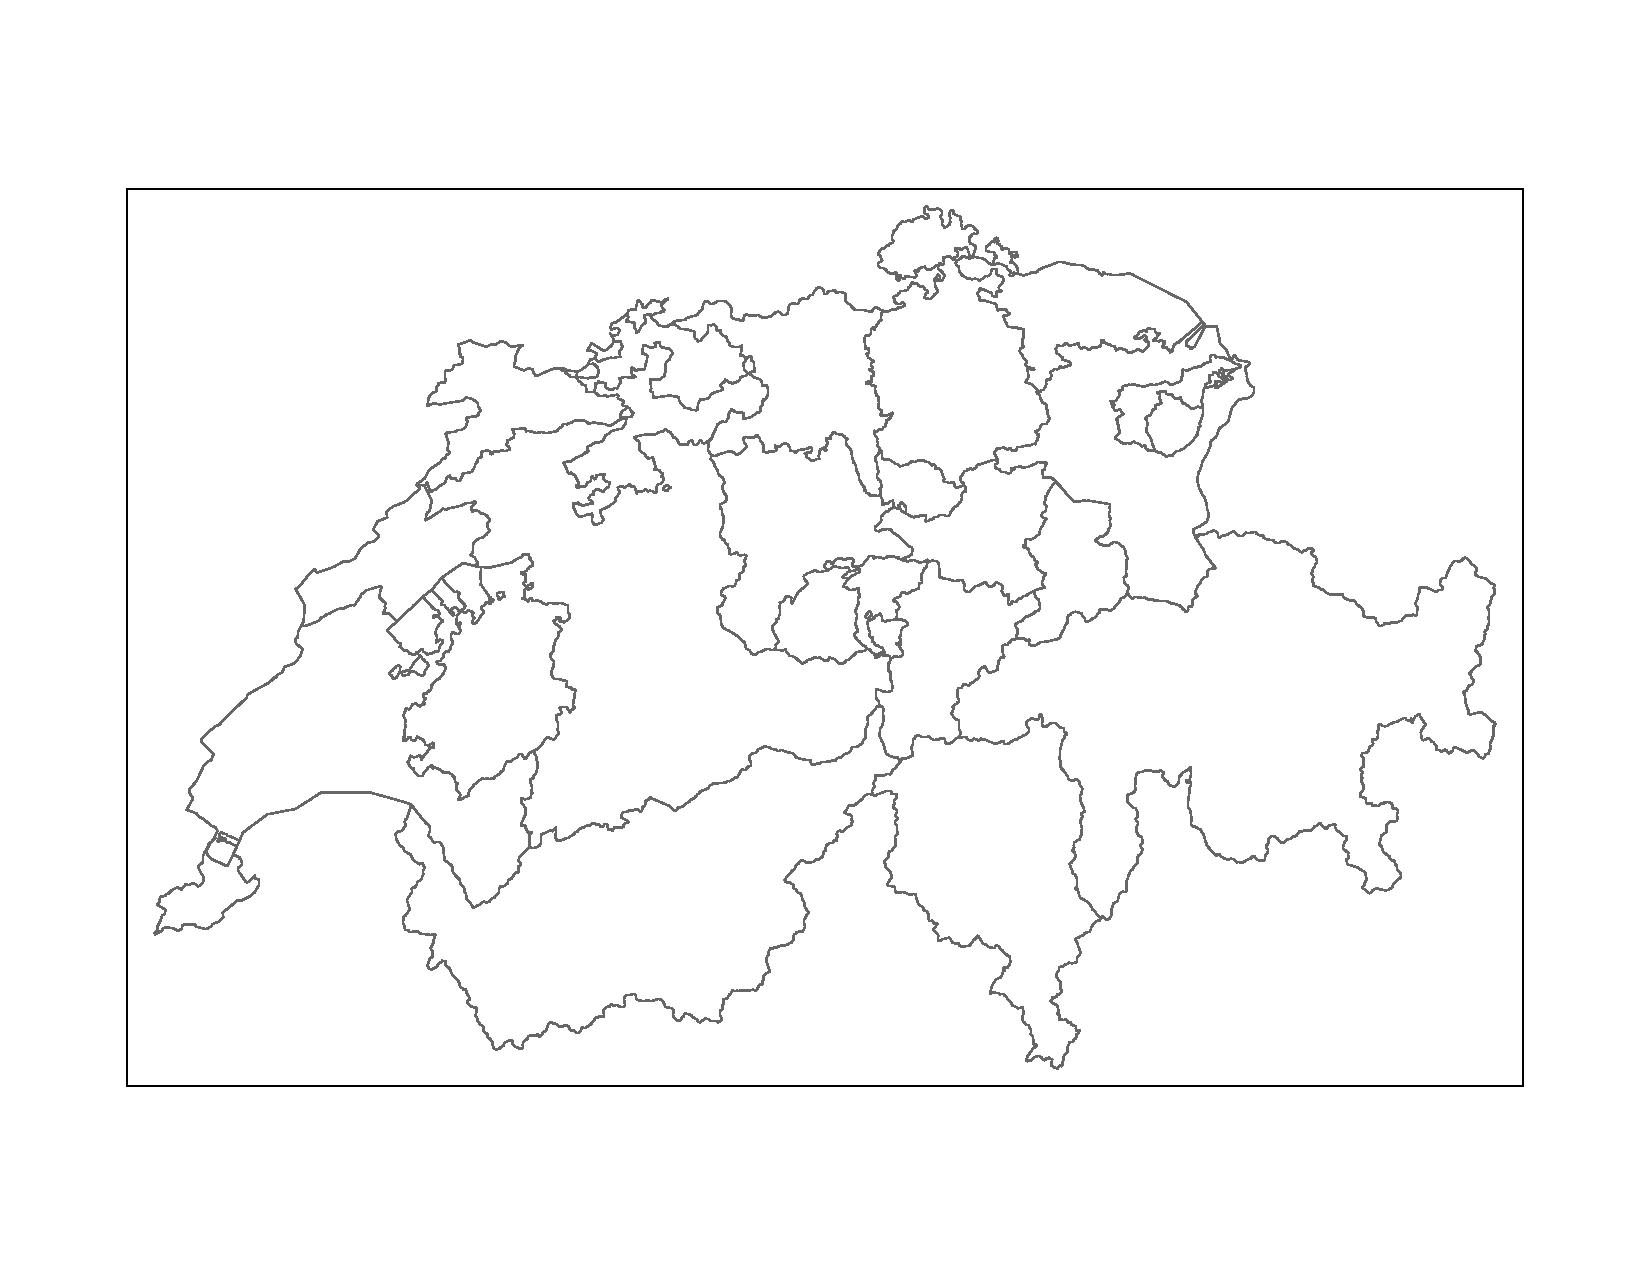
\includegraphics[page=1,width=.7\textwidth]{switzerland.pdf}
 \caption{The cantons of Switzerland, an example of an irregular lattice.}
 \label{fig:lattice}
\end{figure}
\subsection{General Notation and Abbreviations}
For $C\in\mathcal{I}=\left\lbrace1,...,n\right\rbrace$ let $\pmb{y}_C=\left\lbrace y_i:i\in C\right\rbrace$. $-C$ denotes the set $\mathcal{I-C}$ such that $\pmb{y}_{-C}=\left\lbrace y_i:i\notin C\right\rbrace$. For two sets $A$ and $B$, $A\setminus B=\left\lbrace i:i\in A \hbox{ and } i \notin B\right\rbrace$. \\
$\pi\left(\cdot\right)$ denotes the density of its arguments, for example $\pi\left(\pmb{y}\right)$ for the density of $\pmb{y}$ and $\pi\left(\pmb{y}_A|\pmb{y}_{-A}\right)$ for the conditional density of $\pmb{y}_A$, given $\pmb{y}_{-A}$. '$\sim$' is used when a variable is 'distributed' according to the law $l$ \autocite[][16]{rue2005gaussian}.
\subsection{Symmetric Positive Definite Matrices}
An $n \times n$ matrix $\pmb{A}$ is \textit{positive definite} exactly if
\begin{equation*}
    \pmb{x}^T\pmb{A}\pmb{x}>0,\hspace{20pt}\forall\pmb{x}\neq\pmb{0}.
\end{equation*}
If $\pmb{A}$ is also symmetric, it is called a symmetric positive definite (SPD) matrix. Only SPD matrices are considered and sometimes the notation '$\pmb{A}>0$' is used for an SPD matrix $\pmb{A}$. \\
An SPD matrix $\pmb{A}$ has some of the following properties.
\begin{itemize}
    \item[1.] $\hbox{rank}\left(\pmb{A}\right)=n$.
    \item[2.] $|\pmb{A}|>0$.
    \item[3.] $A_{ii}>0$.
    \item[4.] $A_{ii}A_{jj}-A_{ij}^2>0$, for $i\neq j$.
    \item[5.] $A_{ii} + A_{jj}-2|A_{ij}|>0$ for $i\neq j$.
    \item[6.] $\max A_{ii}>\max_{i\neq j}|A_{ij}|$.
    \item[7.] $\pmb{A}^{-1}$ is SPD.
    \item[8.] All principal submatrices of $\pmb{A}$ are SPD.
\end{itemize}
If $\pmb{A}$ and $\pmb{B}$ are SPD, $\pmb{A}+\pmb{B}$ is also SPD, but the reverse is generally not true. Additionally, if $\pmb{AB}=\pmb{BA}$, $\pmb{AB}$ is SPD. \\
The following conditions are all sufficient and necessary for a symmetric matrix $\pmb{A}$ to be SPD:
\begin{itemize}
    \item[1.] All eigenvalues $\lambda_1,...,\lambda_n$ of $\pmb{A}$ are strictly positive.
    \item[2.] There exists such a matrix $\pmb{C}$ that $\pmb{A}=\pmb{CC}^T$. If $\pmb{C}$ is lower triangular, it is called the \textit{Cholesky triangle} of $\pmb{A}$.
    \item[3.] All leading principal submatrices have strictly positive determinants.
\end{itemize}    
A sufficient, but not necessary condition for a (symmetrical) matrix to be SPD is the criterion of \textit{diagonal dominance}:
    \begin{equation*}
        A_{ii}-\sum_{j:j\neq i}|A_{ij}|>0,\hspace{20pt}\forall i.
    \end{equation*}
    A $n\times n$ matrix $\pmb{A}$ is called a \textit{symmetric positive semidefinite} (SPSD) matrix. An SPSD matrix $\pmb{A}$ is sometimes denoted '$\pmb{A}\geq0$' \autocite[][18--19]{rue2005gaussian}.
\clearpage
\section{Basic Concepts of Bayesian Theory}
\subsection{Bayes' Theorem}
At the heart of Bayesian inference is \textit{Bayes' theorem}, which describes the probability of an event given prior knowledge of factors that might influence the event. \\
Let $\pmb{y}^T=\left(y_1,...,y_n\right)$ be a vector of $n$ observations whose probability distribution $\pi\left(\pmb{y}|\pmb{\theta}\right)$ depends on the values of $k$ parameters $\pmb{\theta}^T=\left(\theta_1,...,\theta_k\right)$. Let $\pi\left(\pmb{\theta}\right)$ be the probability distribution of $\pmb{\pmb{\theta}}$. Then 
\begin{equation}
    \pi\left(\pmb{y}|\pmb{\theta}\right)\pi\left(\pmb{\theta}\right)=\pi\left(\pmb{y},\pmb{\theta}\right) = \pi\left(\pmb{\theta}|\pmb{y}\right)\pi\left(\pmb{y}\right).
\end{equation}
Given the observed data $\pmb{y}$, the conditional distribution of $\pmb{\theta}$ is
\begin{equation}
    \pi\left(\pmb{\theta}|\pmb{y}\right)=\frac{p\left(\pmb{y}|\pmb{\theta}\right)\pi\left(\pmb{\theta}\right)}{\pi\left(\pmb{y}\right)}.
\end{equation}
This last statement is known as Bayes' theorem \autocite[][]{bayes1763lii}. The \textit{prior} distribution $\pi\left(\pmb{\theta}\right)$ contains knowledge about $\pmb{\theta}$ without knowledge of the data. $\pi\left(\pmb{\theta}|\pmb{y}\right)$ contains what is known about $\pmb{\theta}$ given knowledge of the data and is the \textit{posterior} distribution of $\pmb{\theta}$ given $\pmb{y}$. \\
If $\pi\left(\pmb{y}|\pmb{\theta}\right)$ is considered as a function of $\pmb{\theta}$ instead of $\pmb{y}$, it is called the \textit{likelihood function} of $\pmb{\theta}$ given $\pmb{y}$ and can be written as $l\left(\pmb{\theta}|\pmb{y}\right)$. Thus Bayes' theorem can be written as
\begin{equation}
    \pi\left(\pmb{\theta}|\pmb{y}\right)\propto l\left(\pmb{\theta}|\pmb{y}\right)\pi\left(\pmb{\theta}\right).
\end{equation}
It is evident that the posterior distribution of $\pmb{\theta}$ given the data $\pmb{y}$ is proportional to the product of the distribution of $\pmb{\theta}$ prior to observing the data and the likelihood function of $\pmb{\theta}$ given $\pmb{y}$. Therefore,
\begin{equation*}
    \hbox{posterior distribution} \propto  \hbox{likelihood}\times\hbox{prior distribution}.
\end{equation*}
The data $\pmb{y}$ modifies the prior knowledge of $\pmb{\theta}$ through the likelihood function, and thus can be be regarded as a representation of the information about  $\pmb{\theta}$ derived from the data \autocite[][]{box2011bayesian}.
\subsection{Conditional Independence}
In probability theory, two random variables $x$ and $y$ are \textit{independent} given a third variable $z$ if and only if the occurrence of $x$ and $y$ in their conditional probability distribution given $z$ are independent events. To calculate the conditional density of $\pmb{x}_A$, given $\pmb{x}_{-A}$, the following statement will repeatedly be used,
\begin{equation}
    \pi\left(\pmb{x}_A|\pmb{x}_{-A}\right)=\frac{\pi\left(\pmb{x}_A,\pmb{x}_{-A}\right)}{\pi\left(\pmb{x}_{-A}\right)}\propto \pi\left(\pmb{x}\right).
\end{equation}
It follows that $x$ and $y$ are independent precisely when $\pi\left(x,y\right)=\pi\left(x\right)\pi\left(y\right)$, which is expressed by $x\perp y$. $x$ and $y$ are conditionally independent for a given $z$ if and only if $\pi\left(x,y|z\right)=\pi\left(x|z\right)\pi\left(y|z\right)$ \autocite[][]{dawid1979conditional}. The conditional independence can be easily validated with the help of the following \textit{factorisation criterion},
\begin{equation}
    x\perp y|z\Longleftrightarrow \pi\left(x,y,z\right)=f\left(x,z\right)g\left(y,z\right),
\end{equation}
for some functions $f$ and $g$, and for all $z$ with $\pi\left(z\right) >0$ \autocite[][16--17]{rue2005gaussian}.
\subsection{Undirected Graphs}
Undirected graphs are used to represent the conditional independence structure in a Gaussian Markov random field. An \textit{undirected graph} $\mathcal{G}$ is defined as a tuple $\mathcal{G}=\left(\mathcal{V}, \mathcal{E}\right)$, where $\mathcal{V}$ contains all nodes in the graph and $\mathcal{E}$ is the set of edges $\left\lbrace i,j\right\rbrace$, with $i,j\in\mathcal{V}$ and $i\neq j$. For $\left\lbrace i,j\right\rbrace \in\mathcal{E}$ there exists an undirected edge from node $i$ to node $j$ in the other case such an edge does not exist. If $\left\lbrace i,j\right\rbrace\in\mathcal{E}\,\,\forall i,j\in\mathcal{V}$ with $i\neq j$ a graph is \textit{fully connected}. Most often $\mathcal{V}=\left\lbrace1,2,...,n\right\rbrace$ will be assumed, which is referred to as \textit{labelled}. A simple example of an undirected graph is shown in \autoref{fig:und_graph}.
\begin{figure}[H]
    \centering
    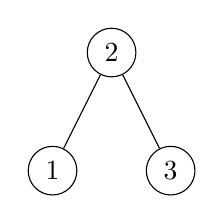
\begin{tikzpicture}[nodes={draw, circle}, -]
    \node{2}
    child { node {1} }
    child { node {3} };
    \end{tikzpicture}
    \caption{An undirected labelled graph with 3 nodes, $\mathcal{V}=\left\lbrace1,2,3\right\rbrace$ and $\mathcal{E}=\left\lbrace\left\lbrace1,2\right\rbrace\left\lbrace2,3\right\rbrace\right\rbrace$.}
    \label{fig:und_graph}
\end{figure} $\newline$
The \textit{neighbours} of node $i$ are defined as all nodes in $\mathcal{G}$ with an edge to node $i$,
\begin{equation*}
    \hbox{ne}\left(i\right)=\left\lbrace j\in\mathcal{V}:\left\lbrace i,j\right\rbrace\in\mathcal{E}\right\rbrace.
\end{equation*}
This definition can be extended to a set $A\subset\mathcal{V}$, where the neighbours of $A$ are defined as
\begin{equation*}
    \hbox{ne}\left(A\right)=\bigcup_{i\in A}\hbox{ne}\left(i\right)\setminus A.
\end{equation*}
A \textit{path} from $i_1$ to $i_m$ is defined as a sequence of certain nodes in $\mathcal{V}, i_1,i_2,...,i_m$, for which $\left(i_j,i_{j+1}\right)\in\mathcal{E}$ for $j=1,...,m-1$. Two nodes $i\notin C$ and $j\notin C$ are \textit{separated} by a subset $C\subset\mathcal{V}$, if every path from $i$ to $j$ contains at least one node from $C$. Two disjoint sets $A\subset\mathcal{V}\notin C$ and $B\subset\mathcal{V}\notin C$ are separated by $C$, if all $i\in A$ and $j\in B$ are separated by $C$, that is, it is not possible to "wander" on the graph from somewhere in $A$ and end somewhere in $B$ without crossing $C$.\\
If $i$ and $j$ are neighbours in $\mathcal{G}$, this can be expressed by $i\overset{\mathcal{G}}{\sim}j$ or $i\sim j$ for the case where the graph is implicit. It follows that $i\sim j\Longleftrightarrow j\sim i$. \\
Let $A$ be a subset of $\mathcal{V}$. A \textit{subgraph} $\mathcal{G}^A$ is a graph restricted to $A$, i.e., the graph obtained after removing all nodes that do not belong to $A$ and all edges where at least one node does not belong to $A$. $\mathcal{G}^A=\left\lbrace\mathcal{V}^A,\mathcal{E}^A\right\rbrace$, where $\mathcal{V}^A=A$ and 
\begin{equation*}
    \mathcal{E}^A = \left\lbrace\left\lbrace i,j\right\rbrace\in\mathcal{A} \hbox{ and } \left\lbrace i,j\right\rbrace\in A\times A\right\rbrace.
\end{equation*}
Let $\mathcal{G}$ be the graph in \autoref{fig:und_graph} and $\mathcal{A}=\left\lbrace2,3\right\rbrace$, then $\mathcal{V}^A=\left\lbrace2,3\right\rbrace$ and $\mathcal{E}^A=\left\lbrace\left\lbrace 2,3\right\rbrace\right\rbrace$ \autocite[][17--18]{rue2005gaussian}.
\subsection{The Exponential Family}
In statistics and probability theory, the \textit{exponential family} is a parametric set of probability distributions of a specific form. The distribution of a random variable $\pmb{y}$ belongs to the exponential family if the discrete or continuous density with respect to a $\sigma$-finite measure of $\pmb{y}$ has the form
\begin{equation}
    f(\pmb{y}|\pmb{\theta}, \lambda)=\exp\left(\frac{\pmb{y}^T\pmb{\theta} - b(\pmb{\theta})}{\lambda}+c(\pmb{y},\lambda) \right),
\end{equation}
with $c(\pmb{y},\lambda)\geq 0$. %and measurable. 
$\pmb{\theta}\in\Theta\subset\mathbb{R}^q$ is the \textit{natural} or \textit{canonical} parameter of the exponential family, while $\lambda > 0$ is a \textit{dispersion} or \textit{nuisance} parameter \autocite[][]{holland1981exponential}. The natural parameter space $\Theta$ is the set of all $\pmb{\theta}$ satisfying
\begin{equation}
    0<\int\exp\left(\left(\pmb{y}^T\pmb{\theta} - b(\pmb{\theta})\right)/\lambda+c(\pmb{y},\lambda) \right)d\pmb{y}< \infty
\end{equation} Moreover, $b(\pmb{\theta})$ is a twice differentiable  function and all moments of $\pmb{y}$ exist. Specifically, 
\begin{alignat}{3}
    \mathbb{E}_{\pmb{\theta}}(\pmb{y}) &= \mu(\pmb{\theta}) =& \frac{\partial b(\pmb{\theta})}{\partial\pmb{\theta}} \\
    \hbox{Cov}_{\pmb{\theta}}(\pmb{y}) &= \pmb{\Sigma}(\pmb{\theta}) =& \lambda\frac{\partial^2b(\pmb{\theta})}{\partial\pmb{\theta}\partial\pmb{\theta}^T}.
\end{alignat}
The covariance matrix $\pmb{\Sigma}(\pmb{\theta})$ is positive definite in $\Theta^0$, therefore $\mu:\Theta^0\rightarrow  M = \mu\left(\Theta^0\right)$ is injective. By substituting the inverse function $\pmb{\theta}(\mu)$ into $\frac{\partial^2b(\pmb{\theta})}{\partial\pmb{\theta}\partial\pmb{\theta}^T}$, the variance function 
\begin{equation}
    v(\mu)=\frac{\partial^2b(\pmb{\theta}(\mu))}{\partial\pmb{\theta}\partial\pmb{\theta}^T}
\end{equation}
is given and the covariance can be written as
\begin{equation}
    \hbox{Cov}_{\pmb{\theta}}(\pmb{y}) = \lambda v(\mu).
\end{equation}
Important members of the exponential family are the normal, binomial, Poisson, gamma and multivariate normal distribution \autocite[][433]{fahrmeir2013multivariate}.
\subsection{The Multivariate Normal Distribution}
The density of a normally distributed random variable $\pmb{y}=\left(y_1,...,y_n\right)^T, n<\infty$ with mean vector $\pmb{\mu}$ ($n\times1$) and SPD covariance matrix $\pmb{\Sigma}$ ($n\times n$) is
\begin{equation}
    \pi\left(\pmb{y}\right)=\left(2\pi\right)^{-n/2}|\pmb{\Sigma}|^{-1/2}\exp\left(-\frac{1}{2}\left(\pmb{y}-\pmb{\mu}\right)^T\pmb{\Sigma}^{-1}\left(\pmb{y}-\pmb{\mu}\right)\right),\hspace{5pt}\pmb{y}\in\mathbb{R}^n
\end{equation}
Here, $\mu_i=\mathbb{E}\left[y_i\right]$, $ \Sigma_{ij}=\hbox{Cov}\left(y_i,y_j\right)$, $ \Sigma_{ii}=\hbox{Var}\left(y_i\right) > 0$ and $\hbox{Corr}\left(y_i,y_j\right)=\Sigma_{ij}/\left(\Sigma_{ii}\Sigma_{jj}\right)^{1/2}$. This is written as $\pmb{y}\sim\mathcal{N}\left(\pmb{\mu},\pmb{\Sigma}\right)$. For $n=1$, $\mu=0$ and $\Sigma_{11}=1$ the standard normal distribution is obtained. \\
$\pmb{y}$ is now split up into $\pmb{y}=\left(\pmb{y}_{\pmb{A}}^T,\pmb{y}_{\pmb{B}}^T\right)$ and $\pmb{\mu}$ and $\pmb{\Sigma}$ are divided accordingly:
\begin{equation*}
    \pmb{\mu} = \begin{pmatrix}\pmb{\mu}_{\pmb{A}} \\ \pmb{\mu}_{\pmb{B}}\end{pmatrix} \hspace{20pt}\hbox{ and }\hspace{20pt} \pmb{\Sigma}=\begin{pmatrix}\pmb{\Sigma}_{\pmb{AA}} & \pmb{\Sigma}_{\pmb{AB}}\\\pmb{\Sigma}_{\pmb{BA}} & \pmb{\Sigma}_{\pmb{BB}}\end{pmatrix}.
\end{equation*}
Some basic properties of the multivariate normal distribution are the following.
\begin{itemize}
    \item[1.] $\pmb{y}_{\pmb{A}}\sim\mathcal{N}\left(\pmb{\mu}_{\pmb{A}}, \pmb{\Sigma}_{\pmb{AA}}\right)$.
    \item[2.] $\pmb{\Sigma}_{\pmb{AB}}=\pmb{0}$ precisely when $\pmb{y}_{\pmb{A}}$ and $\pmb{y}_{\pmb{B}}$ are independent.
    \item[3.] The conditional distribution $\pi\left(\pmb{y}_{\pmb{A}}|\pmb{y}_{\pmb{B}}\right)$ is $\mathcal{N}\left(\pmb{\mu}_{\pmb{A}|\pmb{B}}, \pmb{\Sigma}_{\pmb{A}|\pmb{B}}\right)$, where
    \begin{align*}
        \pmb{\mu}_{\pmb{A}|\pmb{B}} &= \pmb{\mu}_{\pmb{A}}+\pmb{\Sigma}_{\pmb{AB}}\pmb{\Sigma}_{\pmb{BB}}^{-1}\left(\pmb{y}_{\pmb{B}}-\pmb{\mu}_{\pmb{B}}\right) \hbox{ and} \\
        \pmb{\Sigma}_{\pmb{A}|\pmb{B}} &= \pmb{\Sigma}_{\pmb{AA}}-\pmb{\Sigma}_{\pmb{AB}}\pmb{\Sigma}_{\pmb{BB}}^{-1}\pmb{\Sigma}_{\pmb{BA}}.
    \end{align*}
    \item[4.] If $\pmb{y}\sim\mathcal{N}\left(\pmb{\mu}, \pmb{\Sigma}\right)$ and $\pmb{y}'\sim\mathcal{N}\left(\pmb{\mu'}, \pmb{\Sigma'}\right)$ are independent, 
    \item[]then $\pmb{y}+\pmb{y'}\sim\mathcal{N}\left(\pmb{\mu}+ \pmb{\mu'}, \pmb{\Sigma}+ \pmb{\Sigma'}\right)$ \autocite[][19--20]{rue2005gaussian}.
\end{itemize}
\subsection{Skewness}
Skewness is a statistical indicator that describes the type and strength of the asymmetry of a probability distribution. It shows whether and how strongly the distribution is skewed to the right (right-skewed, left-skewed, negative skewness) or to the left (left-skewed, right-skewed, positive skewness). Any non-symmetrical distribution is called skewed. \\
The skewness of a random variable $X$ is the third standardized moment, defined as
\begin{equation}\label{eq:skewness}
    \hbox{Skew}[X]=\mathbb{E}\left[\left(\frac{X-\mu}{\sigma}\right)^3\right] = \frac{\mathbb{E}\left[\left(X-\mu\right)^3\right]}{\left(\mathbb{E}\left[\left(X-\mu\right)^{3/2}\right]\right)^2}=\frac{\mu_3}{\sigma^3},
\end{equation}
with $\mu_3$ the third central moment and $\sigma$ the standard deviation \autocite[][]{doane2011measuring, wilkins1944note}.
\subsection{Kurtosis}
Kurtosis is a measure of the slope of a probability distribution of a random variable. Distributions with low kurtosis scatter relatively evenly; for distributions with high kurtosis, the scatter results more from extreme but rare events. \\
The kurtosis of a random variable $X$ is the fourth standardized moment, defined as
\begin{equation}\label{eq:kurtosis}
    \hbox{Kurt}[X]=\mathbb{E}\left[\left(\frac{X-\mu}{\sigma}\right)^4\right] = \frac{\mathbb{E}\left[\left(X-\mu\right)^4\right]}{\left(\mathbb{E}\left[\left(X-\mu\right)^2\right]\right)^2}=\frac{\mu_4}{\sigma^4},
\end{equation}
with $\mu_4$ the fourth central moment and $\sigma$ the standard deviation \autocite[][]{decarlo1997meaning, wilkins1944note}.
\clearpage
\section{Prior Selection}
A key question in Bayesian analysis is the effect of the prior on the posterior, and how that effect can be measured. Do posterior distributions derived with different priors become very similar as more and more data is collected? It has been formally proven that under certain regularity conditions, the impact of the prior decreases with increasing sample size. From a practical point of view, it is more important to know what happens when the sample size $n$ is finite. In this section, different types of priors are introduced.
\subsection{Conjugate Priors}
One property of exponential families is that they have conjugate priors \autocite[][]{diaconis1979conjugate}, which is an important property in Bayesian statistics. If the posterior distribution $\pi\left(\pmb{\theta}|\pmb{y}\right)$ and the prior distribution $\pi\left(\pmb{\theta}\right)$ belong to the same probability distribution family, the prior and posterior distributions are called \textit{conjugate} distributions. Furthermore, the prior for the likelihood function $\pi\left(\pmb{y}|\pmb{\theta}\right)$ is called the \textit{conjugate prior}. These priors were first discussed and formalised by Raifa and Schlaifer in 1961 \autocite[][]{raiffaapplied}. \\
The construction of a conjugate prior is done by factorising the likelihood function into two parts. One part must be independent of the parameter(s) of interest but can be dependent on the data, while the other factor is a function that depends on the parameter(s) of interest and is dependent on the data only through the sufficient statistics. The family of conjugate priors is by definition proportional to the second factor. The posterior distribution resulting from the conjugate prior is itself a member of the same family as the conjugate prior \autocite[][]{raiffaapplied}. In cases where the prior and posterior distributions are part of the same family, the prior is said to be closed under sampling. Furthermore, since the data are only incorporated into the posterior distribution through the sufficient statistics, there exist relatively simple formulas for updating the prior into the posterior.\\
For an example of the construction of a conjugated prior, see Fink 1997 \autocite[][]{fink1997compendium}.\\
A drawback of conjugated priors is that the a priori known information about $\mu$ may be insufficient for determining both parameters or may be inconsistent with the structure imposed by conjugacy \autocite[][]{robert2010bayesian}. Moreover, these priorities can be too restrictive and not every belief about the priori can be described \autocite[][]{irwin2005prior}. \\
Thus, although conjugate priors are easy to handle both mathematically and computationally \autocite[][]{irwin2005prior}, they are not often used in practice because of these drawbacks.
% \subsection{Jeffreys' Prior}
% As conjugate priors depend on information from the data, they are so-called \textit{informative priors}. \textit{Jeffreys' prior} \autocite[][]{jeffreys1946invariant} is characterised in comparison to other a priori distributions by the fact that it is invariant to a reparametrisation of the model parameters. Due to this invariance, the Jeffreys' a priori distribution is also called \textit{non-informative}. \\
% Let $\phi=\phi\left({\theta}\right)$ be a one-to-one transformation of ${\theta}$ and $I\left(\cdot\right)$ be the Fisher information, then
% \begin{equation}
%     I_{\phi}\left(\phi\right)=I_{\theta}\left({\theta}\right)\left(\frac{\partial{\theta}}{\partial\phi}\right)^2.
% \end{equation}
% If some principle of choice led to $\pi\left(\theta\right)$ as a non-informative prior for $\theta$, the same principle should lead to
% \begin{equation}
%     \pi_{\phi}\left(\phi\right)=\pi_{\theta}\left(\theta\right)\left|\frac{\partial\theta}{\partial\phi}\right|
% \end{equation}
% as a non-informative prior for $\phi$. The desired "invariance" is then given by
% \begin{equation}
%     \pi_{\phi}\left(\phi\right)\propto \sqrt{I_{\phi}\left(\phi\right)}=\sqrt{I_{\theta}\left(\theta\right)}\left|\frac{\partial\theta}{\partial\phi}\right|\propto \pi_{\theta}\left(\theta\right)\left|\frac{\partial\theta}{\partial\phi}\right|
% \end{equation}
% \autocite[][42--43]{box2011bayesian}. While Jeffreys' priors work well for single parameter models, they struggle when it comes to models with multidimensional parameters as these priors can have poor convergence properties \autocite[][]{jordan2010}.
\subsection{Penalised Complexity Priors}
One issue when selecting the prior distribution of a particular parameter is that it is not always intuitive when it comes to understanding and interpreting this distribution, something that is essential to ensure that it behaves as intended by the user. This problem can be addressed by using \textit{penalised complexity priors}, which is a methodology that penalises the complexity of model components in relation to deviation from simple base model formulations.\\
PC priors provide a systematic and unified approach to calculating priority distributions for parameters of model components by using an inherited nested structure. This structure contains two models, the base model and a flexible version of the model. The first of the two is generally characterised by a fixed value of the relevant parameter, while the second version is considered a function of the random parameter. By penalising the deviation from the flexible model to the fixed base model, the PC prior is calculated \autocite[][]{martins2014penalising}.
\subsubsection{The Principles Behind PC Priors}
Four main principles should be followed to calculate priors in a consistent way and to understand their properties.
\subsubsection*{Support to Occam's Razor} 
Let $\pi\left(x|\xi\right)$ denote the density of a model component $x$ and $\xi$ the parameter to which a prior distribution is to be assigned. The base model is characterised by a density $\pi\left(x|\xi=\xi_0\right)$, where $\xi_0$ is a fixed value. The prior for $\xi$ should be such that proper shrinkage is given to $\xi_0$. The simplicity of the model is therefore prioritised over the complexity of the model, preventing overfitting \autocite[][]{martins2014penalising}.
\subsubsection*{Penalisation of Model Complexity} 
Let $f_1=\pi\left(x|\xi\right)$ and $f_0\left(x|\xi=\xi_0\right)$ denote the flexible model and the base model respectively. The complexity of $f_1$ compared to $f_0$ is characterised using the Kullback-Leibler divergence \autocite[][]{kullback1951information} to calculate a measure of complexity between the two models,
\begin{equation}
    \hbox{KLD}\left(f_1||f_2\right) = \int f_1\left(x\right)\log\left(\frac{f_1\left(x\right)}{f_0\left(x\right)}\right)dx.
\end{equation}
This can be used to measure the information that is lost when $f_1$ is approximated by the simpler model $f_0$. For multinormal densities with zero mean, the calculation simplifies to
\begin{equation}
    \hbox{KLD}\left(f_1||f_0\right) = \frac{1}{2}\left(\hbox{trace}\left(\pmb{\Sigma}_0^{-1}\pmb{\Sigma}_1\right)-n-\log\left(\frac{\left|\pmb{\Sigma}_1\right|}{\left|\pmb{\Sigma}_0\right|}\right)\right),
\end{equation}
where $f_i\sim\mathcal{N}\left(0,\pmb{\Sigma}_i\right), i=0,1$, while $n$ represents the dimension. For easier interpretation, the Kullback-Leibler divergence is transformed into a unidirectional distance measure
\begin{equation}
    d\left(\xi\right) = d\left(f_1||f_0\right)=\sqrt{2\hbox{KLD}\left(f_1||f_0\right)}
\end{equation}
which can be interpreted as a measure of distance from $f_1$ to $f_0$ \autocite[][]{martins2014penalising}.
\subsubsection*{Constant Rate Penalisation}
The derivation of the PC prior is based on a system of constant rate penalisation, given by
\begin{equation}
    \frac{\pi_d\left(d\left(\xi\right)+\delta\right)}{\pi_d\left(d\left(\xi\right)\right)}=r^{\delta}, \hspace{20pt} d\left(\xi\right),\delta\geq0.
\end{equation}
$r\in\left(0,1\right)$ represents the constant decay rate and thus implies that the relative change in the priority distribution for $d\left(\xi\right)$ is independent of the actual distance. Therefore, $d\left(\xi\right)$ is exponentially distributed with density $\pi\left(d\left(\xi\right)\right)=\lambda\exp\left(-\lambda d\left(\xi\right)\right)$ and rate $\lambda = -\ln\left(r\right)$. By a standard variable change transformation, the corresponding PC prior for $\xi$ is given \autocite[][]{martins2014penalising}.
\subsubsection*{User-Defined Scaling}
Since $\lambda$ characterises the shrinkage properties of the prior, it is important that the rate can be chosen in an intuitive and interpretable way. One possibility is to determine $\lambda$ by including a probability statement of tail events, for example
\begin{equation}\label{eq:pcprior}
    \mathbb{P}\left(Q\left(\xi\right) > U\right)=\alpha,
\end{equation}
where $U$ represents an assumed upper bound for an interpretable transformation $Q\left(\xi\right)$ and $\alpha$ denotes a small probability \autocite[][]{martins2014penalising}.
% \subsubsection{PC Priors for AR(1)}
% The first-order AR process is given by
% \begin{equation}
%     x_t=\phi x_{t-1}+\epsilon_t, \hspace{20pt}\epsilon\sim\mathcal{N}\left(0, \kappa^{-1}\right), \hspace{5pt} t=2,...,n,
% \end{equation}
% where $x_1$ is assumed to follow a normal distribution with mean $0$ and marginal precision $\tau=\kappa\left(1-\phi^2\right)$. The variables $\left\lbrace\epsilon_t\right\rbrace_{t=1}^n$ are independent and follow a $\mathcal{N}\left(0, \kappa\right)$ distribution. The AR(1) model represents an important special case of AR processes where the autocorrelation coefficient $\phi$ specifies the complete dependence structure. For the precision parameter $\tau$ a type 2 Gumbel distribution is used as PC prior:
% \begin{equation*}
%    \pi\left(\tau\right)=\frac{\lambda}{2}\tau^{-3/2}\exp\left(-\lambda\tau^{-1/2}\right), \hspace{10pt}\lambda>0.
% \end{equation*}
% This prior is derived using infinite precision as the base model, following Simpson et. al (2017) \autocite[][]{martins2014penalising}. The rate $\lambda$ is inferred through $\mathbb{P}\left(1/\sqrt{\tau} > U\right)=\alpha$, with $\alpha$ denoting a small probability \autocite[][]{sorbye2017penalised}.
% \subsubsection*{Base Model: No Dependency in Time} 
% The correlation matrix of an AR(1) is generally defined as $\pmb{\Sigma}_1=\left(\phi^{\left|i-j\right]}\right)$. In the case of no autocorrelation, white noise results and the correlation matrix is equal to the identity matrix, $\pmb{\Sigma}_0=\pmb{I}$. The distance function is defined as $d\left(\phi\right)=\sqrt{\left(1-n\right)\log\left(1-\phi^2\right)}$. According to the constant rate penalty principle, $d\left(\phi\right)$ is assigned an exponential prior with rate $\theta/\sqrt{n-1}$. This leads to a prior distribution that is invariant to $n$, and the PC for the one-lag autocorrelation is given by
% \begin{equation}
%    \pi\left(\phi\right)=\frac{\theta}{2}\exp\left(-\theta\sqrt{-\ln\left(1-\phi^2\right)}\right)\frac{|\phi|}{\left(1-\phi^2\right)\sqrt{-\ln\left(1-\phi^2\right)}}, \hspace{20pt} |\phi|<1,\theta>0.
% \end{equation}
% The rate parameter $\theta$ influences at what rate the prior shrinks towards the white noise base model. To infer $\theta$, a tail event is used. In the case of $\phi = 0$ a tail event can be defined by the fact that large absolute correlations are less likely, i.e..,
% \begin{equation*}
%    \mathbb{P}\left(|\phi|>U\right) = \alpha.
% \end{equation*}
%This implies that $\theta=-\ln\left(\alpha\right)/\sqrt{-\ln\left(1-U^2\right)}$ \autocite[][]{sorbye2017penalised}.
% \subsubsection*{Base Model: No Change in Time} 
% As an alternative to the base model for the AR(1) process, it can be assumed that the process remains constant in time ($\phi = 1$), thus representing a limiting random walk case, which is a non-stationary and singular process. To derive the PC prior for $\phi$, let $\pmb{\Sigma}_1=\left(\phi^{|i-j|}\right)$ and $\pmb{\Sigma}_0=\left(\phi_0^{|i-j|}\right)$, where $\phi_0$ is close to $1$ and $\phi<\phi_0$. The Kullback-Leibler divergence is
% \begin{align*}
%    &\hbox{KLD}\left(f_1\left(\phi\right)||f_0\right)=\\
%    &\frac{1}{2}\left(\frac{1}{1-\phi_0^2}\left(n-2\left(n-1\right)\phi_0\phi+\left(n-2\right)\phi_0^2\right)-n-\left(n-1\right)\ln\left(\frac{1-\phi^2}{1-\phi_0^2}\right)\right).
% \end{align*}
% Considering the limit as $\phi_0\rightarrow1$, the distance is
% \begin{align*}
%    d\left(\phi\right)&=\underset{\phi_0\rightarrow1}{\lim}\sqrt{2\hbox{KLD}\left(f_1\left(\phi\right)||f_0\right)} \\
%    &=\underset{\phi_0\rightarrow1}{\lim}\sqrt{\frac{2\left(n-1\right)\left(1-\phi\right)}{1-\phi_0^2}} = c\sqrt{1-\phi}, \hspace{20pt}|\phi|<1,
% \end{align*}
% constant for $c$, independent of $\phi$. Since $0\leq d\left(\phi\right)\leq c\sqrt{2}$, $d\left(\phi\right)$ is assigned a truncated exponential distribution with rate $\theta/c$, resulting in the following PC prior,
% \begin{equation}
%    \pi\left(\phi\right)=\frac{\theta\exp\left(-\theta\sqrt{1-\phi}\right)}{\left(1-\exp\left(-\sqrt{2}\theta\right)\right)2\sqrt{1-\phi}}, \hspace{20pt}|\phi|<1.
% \end{equation}
% To scale the prior in terms of $\theta$, $\left(U,\alpha\right)$ is determined in terms of $\mathbb{P}\left(\phi>U\right)=\alpha$. This equation is solved by
% \begin{equation*}
%    \frac{1-\exp\left(-\theta\sqrt{1-U}\right)}{1-\exp\left(-\sqrt{2}\theta\right)}=\alpha,
% \end{equation*}
% provided that $\alpha$ is larger than the lower limit $\sqrt{\left(1-U\right)/2}$ % \autocite[][]{sorbye2017penalised}.
\clearpage
\section{Markov-Chain-Monte-Carlo-Methods}
Markov chain Monte Carlo methods, also referred to as MCMC methods, are a set of algorithms that enable sampling from probability distributions based on the construction of Markov chains. After a sufficient number of iterations, the stationary distribution of a Markov chain can be taken as the desired distribution, with the quality of this distribution improving as the number of iterations increases. Most of the time, the construction of such a chain is relatively simple; the real challenge is to determine how many steps are needed before convergence towards the stationary distribution is achieved. MCMC methods are mostly used to compute numerical approximations of multidimensional integrals, for instance in Bayesian statistics or computational biology. The two main concepts used in MCMC methods are Monte Carlo integration and the aforementioned Markov chains, hence the name Markov Chain Monte Carlo.
\subsection{Monte Carlo Integration}
\textit{Monte Carlo integration} is a technique that uses the generation of random numbers for numerical computation of definite integrals and is especially useful for higher-dimensional integrals. The problem the method addresses is the computation of the integral
\begin{equation}
    \mathbb{E}_f\left[h\left(X\right)\right]=\int_\chi h(x)f(x)dx.
\end{equation}
The integral can be approximated by using a sample $\left(X_1,...,X_m\right)$ generated from $f$ and calculating the arithmetic mean
\begin{equation}
    \overline{h}_m=\frac{1}{m}\sum_{j=1}^mh\left(x_j\right).
\end{equation}
According to the Strong Law of Large Numbers, $\overline{h}_m$ is likely to converge to $\mathbb{E}_f\left[h\left(X\right)\right]$. When the expectation of $h^2$ under $f$ is finite, the convergence speed of $\overline{h}_m$ can be assessed. The variance too can be estimated from the sample $\left(X_1,...,X_n\right)$ through
\begin{equation}
    v_m=\frac{1}{m^2}\sum_{j=1}^m\left[h\left(x_j\right)-\overline{h}_m\right]^2.
\end{equation}
For $m$ large,
\begin{equation}
    \frac{\overline{h}_m-\mathbb{E}_f\left[h\left(X\right)\right]}{\sqrt{v_m}}
\end{equation}
is approximately distributed as a $\mathcal{N}(0,1)$ variable. This can be used for constructing a convergence test and to calculate confidence bounds for the approximation of $\mathbb{E}_f\left[h\left(X\right)\right]$ \autocite[][83--84]{robert2013monte}. The term Monte Carlo was first used in 1949 by Metropolis and Ulam to describe a method dealing with problems related to "integro-differential equations that occur in various branches of the natural sciences" \autocite[][]{metropolis1949monte}.
\subsection{Markov Chains}
Markov chains are stochastic processes that aim to provide the probability of the occurrence of future events. A Markov chain is defined by the fact that even if only a limited history is known, predictions about future developments can be made just as reliably as if the entire history of a process were known. Thus, the probability of moving from the current state to any state depends only on the current state of the chain. These probabilities are defined by a \textit{transition kernel}, which is a function $K$ on $\mathcal{X} \times \mathcal{B}\left(\mathcal{X}\right)$, such that
\begin{itemize}
    \item[i.] $\forall x\in\mathcal{X}, K\left(x, \cdot\right)$ is a probability measure;
    \item[ii.] $\forall A\in \mathcal{B}\left(\mathcal{X}\right), K\left(\cdot, A\right)$ is measureable.
\end{itemize}
In the discrete case, the transition kernel is a matrix $\pmb{K}$ with elements
\begin{equation*}
    \mathbb{P}_{xy}=\mathbb{P}\left(X_n=y|X_{n-1}=x\right), \hspace{20pt}x,y\in\mathcal{X}.
\end{equation*}
If $\mathcal{X}$ is continuous, the kernel denotes the conditional density $K\left(x,x^T\right)$ of the transition $K\left(x,\cdot\right)$,
\begin{equation*}
    \mathbb{P}\left(X\in A|x\right)=\int_AK\left(x,x^T\right)dx^T.
\end{equation*}
Given a transition kernel $K$, a sequence $X_0,X_1,...,X_t$ of random variables is a \textit{Markov chain} $\left(X_n\right)$, if, for any $t$, the conditional distribution of $X_t$ given the previous states is the same as the distribution of $X_t$ given the last state, $x_{t-1}$,
\begin{align}
    \mathbb{P}\left(X_{t+1}\in A|x_0,x_1,x_2,...,x_t\right) &= \mathbb{P}\left(X_{t+1}\in A|x_t\right) \nonumber\\
    &= \int_A K\left(x_t, dx\right). 
\end{align}
These chains were first introduced by Markov in 1906 \autocite[][]{markov1906extension}. Markov chains can have certain properties that affect their long-term behaviour and are of particular importance for MCMC algorithms. In sections~\ref{sssec:irreducibility}--~\ref{sssec:stationary}, some of them will be introduced.
\subsubsection{Irreducibility} \label{sssec:irreducibility}
Irreducibility is critical to the construction of Markov chain Monte Carlo algorithms, as it ensures the convergence of such an algorithm. A Markov chain is \textit{irreducible} if all states communicate, that is, for all states $i$ and $j$ the probability of getting from $i$ to $j$ in finite time is true positive. \\
Formally speaking, given a measure $\varphi$, a Markov chain $\left(X_n\right)$ with transition kernel $K\left(x,y\right)$ is $\varphi$-\textit{irreducible}, if, for every $A\in B\left(\mathcal{X}\right)$ with $\varphi\left(A\right)>0$, there exists $n$ such that $K^n\left(x,A\right) \forall x\in\mathcal{X}$. The chain is \textit{strongly} $\varphi$-\textit{irreducible} if $n=1\forall$ measurable $A$ \autocite[][213--214]{robert2013monte}.
\subsubsection{Periodicity} 
The behaviour of a Markov chain can sometimes be limited by deterministic constraints on the transitions from $X_n$ to $X_{n+1}$. For discrete chains, the \textit{period} of a state $w\in\mathcal{X}$ is defined as. 
\begin{equation*}
    d\left(w\right)=\hbox{g.c.d. } \lbrace m\geq 1;K^m\left(w,w\right)>0\rbrace,
\end{equation*}
with g.c.d the greatest common denominator. If a Markov chain is irreducible, the transition matrix can be written as a block matrix
\begin{equation}
    \pmb{P}=\begin{pmatrix}
    0 & \pmb{D}_1 & 0 & \dots & 0\\
    0 & 0 & \pmb{D}_2 & \dots & 0 \\
    \vdots & \vdots & \ddots  \\
    \pmb{D}_d & 0 & 0 & & 0
    \end{pmatrix},
\end{equation}
It is evident that at every $d$-th step there is a return to the initial group. There exists only one value for the period when a chain is irreducible. If this value is 1, the irreducible chain is \textit{aperiodic} \autocite[][217--218]{robert2013monte}.
\subsubsection{Transience and Recurrence} 
To guarantee an acceptable approximation of a simulated model, a Markov chain needs to have good stability properties. Irreducibility is not strong enough to ensure that the trajectory of $\left(X_n\right)$ enters $A$ often enough. This leads to the formalisation of \textit{recurrence} and \textit{transience}.  \\
In a finite space $\mathcal{X}$, a state $w\in\mathcal{X}$ is \textit{transient} if it is finitely often visited and \textit{recurrent} if it is almost certainly infinitely often visited. \\
For irreducible chains, these two properties are properties of the chain, not of a particular state \autocite[][218--219]{robert2013monte}.
\subsubsection{Ergodicity}
When looking at a Markov chain $\left(X_n\right)$ from a temporal point of view, it is essential to establish to what the chain is converging. A natural candidate for the limiting distribution is the stationary distribution $\pi$ which leads to the need to define sufficient conditions on $\left(X_n\right)$ for $X_n$ to be asymptotically distributed according to $\pi$. There are several conditions that can be imposed on the convergence of $P^n$, the distribution of $X_n$ to $\pi$. The most fundamental and important is that of \textit{ergodicity}, that is, independence of initial conditions.\\
If a Markov chain $\left(X_n\right)$ is both aperiodic and positive recurrent, it is called an \textit{ergodic} Markov chain \autocite[][231--234]{robert2013monte}.
\subsubsection{Stationary distribution} \label{sssec:stationary}
A chain $\left(X_n\right)$ is more stable if the marginal distribution of $X_n$ is independent of $n$. This is a requirement for the existence of a probability distribution $\pi$ such that $X_{n+1}\sim\pi$ if $X_n\sim\pi$. Markov chain Monte Carlo methods rely on the fact that this condition can be satisfied. \\
A $\sigma$-finite measure $\pi$ is \textit{invariant} for the transition kernel $K\left(\cdot,\cdot\right)$ if \begin{equation*}
    \pi\left(B\right)=\int_\mathcal{X}K\left(x,B\right)\pi(dx), \hspace{20pt} \forall B\in\mathcal{B}\left(\mathcal{X}\right).
\end{equation*}
This distribution is referred to as \textit{stationary} if $\pi$ is a probability measure, as $X_0\sim\pi$ implies that $X_n\sim\pi$ is $\forall n$. An irreducible Markov chain has a stationary distribution precisely if it is positively recurrent. The distribution is then given by
\begin{equation}
    \pi_x=\left(\mathbb{E}_x\left[\tau_x\right]\right)^{-1}, \hspace{20pt} x\in\mathcal{X},
\end{equation}
where $\mathbb{E}_x\left[\tau_x\right]$ can be interpreted as the average number of transitions between two passages in $x$. \\
In practice, the stationary distributions are often of special interest. If these distributions are defined as the starting distribution of $X_0$, then all following distributions of the states $X_n$ for any $n$ are equal to the starting distribution. The interesting question here is when such distributions exist and when any distribution converges against a stationary distribution of this kind \autocite[][223--224]{robert2013monte}.
\subsection{The Metropolis-Hastings Algorithm}
Having established the basics of MCMC methods, one of the best known MCMC algorithms, the Metropolis-Hastings algorithm, is introduced next. The algorithm is based on the Metropolis algorithm, which was developed to simulate the states of a system according to the Boltzmann distribution, with the newest state always depending on the previous state \autocite[][]{metropolis1953equation}. \\ 
The Metropolis-Hastings algorithm is a procedure for drawing random samples from a probability distribution from which direct sampling is difficult if a function proportional to the \textit{target density} $f$ is known.
This function $q\left(\pmb{y}|\pmb{x}\right)$ is called the \textit{proposal density} and must be easy to simulate in order for the Metropolis-Hastings algorithm to be implementable. Moreover, it must be either explicitly present or \textit{symmetric}, meaning $q\left(\pmb{x}|\pmb{y}\right)=q\left(\pmb{y}|\pmb{x}\right)$. \\
The Metropolis-Hastings algorithm of a target density $f$ and proposal density $q$ produces a Markov chain $\left(X^{(t)}\right)$ by the following transition.
\begin{algorithm}[H]
\caption{The Metropolis-Hastings Algorithm}
\begin{algorithmic}[1]
\Statex Given $f\left(\pmb{x}\right)$ and $q\left(\pmb{y}|\pmb{x}\right)$
\State Initialisation: Choose arbitrary $x_t$ as the first sample
\For{each iteration $t$}
    \State Generate $Y_t\sim q\left(\pmb{y}|x^{(t)}\right)$
    \State Take 
    \begin{align}
        X^{(t+1)}&=\begin{cases}
        Y_t & \hbox{with probability } \mathbb{P}\left(x^{(t)}, Y_t\right) \\
        x^{(t)} & \hbox{with probability } 1-\mathbb{P}\left(x^{(t)}, Y_t\right)
        \end{cases} \nonumber \\
    \hbox{where} \nonumber\\
    \mathbb{P}\left(x,y\right) &= \min\left\lbrace\frac{f\left(\pmb{y}\right)}{f\left(\pmb{x}\right)}\frac{q\left(\pmb{x}|\pmb{y}\right)}{q\left(\pmb{y}|\pmb{x}\right)}, 1\right\rbrace.
    \end{align} 
    \EndFor
\end{algorithmic}
\end{algorithm}  $\newline$
$\mathbb{P}\left(x,y\right)$ is the \textit{Metropolis-Hastings acceptance probability}. \\
The algorithm always accepts values $y_t$ that lead to an increase in the ratio $f\left(y_t\right)/q\left(y_t|x^{(t)}\right)$ compared to the previous value $f\left(x^{(t)}\right)/q\left(x^{(t)}|y_t\right)$. In the symmetric case, the acceptance probability simplifies to
\begin{equation*}
     \mathbb{P}\left(x,y\right) = \min\left\lbrace\frac{f\left(\pmb{y}\right)}{f\left(\pmb{x}\right)}, 1\right\rbrace
\end{equation*}
\autocite[][]{hastings1970monte}. \\
If the Markov chain starts with a value $x^{(0)} > 0$, then $f\left(x^{(t)}\right) > 0\,\,\forall t\in\mathbb{N}$ since the values of $y$ such that $f\left(y_t\right) = 0$ will all be rejected by the algorithm. As the number of iterations $t$ increases, the distribution of saved states $x_0,...,x_t$ will converge towards the target density $f(\pmb{x})$ \autocite[][270--275]{robert2013monte}.
% hier könnten noch Diagnostics für MCMC methods / MH Algorithm sein, z.b. Traceplot. Außerdem sample mean für schätzung des posterior mean und sample variance für schätzung der varianz
% \subsection{The Gibbs Sampler}
% Gibbs-Sampling is a special case of the Metropolis-Hastings Algorithm, that is used to generate a sequence of samples of the joint probability distribution of two or more random variables. The aim of the method is to approximate this unknown joint probability distribution. Gibbs sampling is especially suitable when the joint distribution of a random vector is unknown, but the conditional distribution of each random variable is known. The underlying principle is to repeatedly select a variable and generate a value according to its conditional distribution, depending on the values of the other variables. During this iteration step, the values of the other variables remain unchanged. A Markov chain can be derived from the resulting sequence of sample vectors, and it can be shown that the stationary distribution of this Markov chain is precisely the sought joint distribution of the random vector. \\
% The Gibbs sampler was first introduced in a 1984 paper by Stuart and Donald Geman \autocite[][]{geman1984stochastic} and is named after the physicist Josiah Willard Gibbs.
% \subsubsection{The Two-Stage Gibbs Sampler}
% A general introduction to Gibbs sampling is the two-stage Gibbs sampler, which is applicable to a wide range of statistical models that do not demand the generality of the multi-stage Gibbs sampler. \\
% Implementing the algorithm is straightforward. If the random variables $X$ and $Y$ have a joint density $f\left(\pmb{x},\pmb{y}\right)$, the two-stage Gibbs sampler generates a Markov chain $\left(X_t,Y_t\right)$ as shown below.
% \begin{algorithm}
% \caption{The Two-Stage Gibbs Sampler}
% \begin{algorithmic}[1]
% \Statex Take $X_0=x_0$
% \For{each iteration $t$}
%    \State Generate $Y_t\sim f_{Y|X}\left(\cdot|x_{t-1}\right)$
%    \State Generate $X_t\sim f_{X|Y}\left(\cdot|y_t\right)$
%    \EndFor
% \end{algorithmic}
% \end{algorithm} 
% $f_{Y|X}$ and $f_{X|Y}$ represent the conditional densities associated with $f$. It is worth noting that not only $\left(X_t,Y_t\right)$ is a Markov chain, but also the subsequences $\left(X_t\right)$ and $\left(Y_t\right)$ are. \autocite[][339]{robert2013monte}.
% \subsubsection*{Normal Bivariate Gibbs Sampler} 
% In the case of the bivariate normal density
% \begin{equation*}
%    \left(X,Y\right)\sim \mathcal{N}_2\left(0,  \begin{pmatrix}
%    1 & p \\ p & 1
%    \end{pmatrix}\right)
% \end{equation*}
% the Gibbs sampler reads as follows:
% \begin{algorithm}
% \caption{The Two-Stage Gibbs Sampler for a normal distribution}
% \begin{algorithmic}[1]
% \Statex Given $y_t$
% \For{each iteration $t$}
%     \State Generate $X_{t+1}|y_t \sim \mathcal{N}\left(py_t, 1-p^2\right)$
%    \State Generate $Y_{t+1}|x_{t+1}\sim\mathcal{N}\left(px_{t+1},1-p^2\right)$
%    \EndFor
% \end{algorithmic}
% \end{algorithm} \\
% \autocite[][340]{robert2013monte}
% \subsubsection{The Multi-Stage Gibbs Sampler}
% Let $p>1$, then the random variable $X\in\mathcal{X}$ can be written as $X=\left(X_1,...,X_p\right)$, where the $X_i$'s are either one-dimensional or multidimensional. Moreover, assume that a simulation is possible from the corresponding univariate conditional densities $f_1,...,f_p$, i.e., 
% \begin{equation*}
%   X_i|\pmb{x}_{-i}\sim f_i\left(x_i|\pmb{x}_{-i}\right)
% \end{equation*}
% can be simulated for $i=1,...,p$. The Gibbs sampler is then specified by the following transition from $X^{(t)}$ to $X^{(t+1)}$:
% \begin{algorithm}[H]
% \caption{The Multi-Stage Gibbs Sampler}
% \begin{algorithmic}[1]
% \Statex Given $x^{(t)}=\left(x_1^{(t)},...,x_p^{(t)}\right)$, generate
% \State $X_1^{(t+1)}\sim f_1\left(x_1|x_2^{(t)},...,x_p^{(t)}\right)$;
% \State $X_2^{(t+1)}\sim f_2\left(x_2|x_1^{(t)},x_3^{(t)},...,x_p^{(t)}\right)$;
% \Statex $\vdots$
% \Statex $X_p^{(p+1)}\sim f_p\left(x_p|\pmb{x}_{-p}\right)$
% \end{algorithmic}
% \end{algorithm} $\newline$
% $f_1,...,f_p$ are referred to as the \textit{full conditionals} and these are the only densities used for simulation. Hence, all simulations can be univariate, even for a high-dimensional problems  \autocite[][371--373]{robert2013monte}.
\clearpage
\section{Latent Gaussian Models and INLA}
In recent years, a growing amount of georeferenced data has become available, leading to an increased need for appropriate statistical modeling to handle large and complex datasets. Bayesian hierarchical models have proven to be effective in capturing complex stochastic structures in spatial processes. A large proportion of these models are based on latent Gaussian models, a subclass of structured additive regression models. These models include Integrated Nested Laplace Approximations (INLA), which are a class of models used to approximate the posterior marginals of a latent Gaussian field. These approximations work by reformulating the regression model as a three-part hierarchical model. The parts are as follows:
\begin{itemize}
    \item[1.] Approximation of the posterior marginal of $\pmb{\theta}$ by using the Laplace approximation.
    \item[2.] Computation of the (simplified) Laplace approximation for selected values of $\pmb{\theta}$ to improve the Gaussian approximation.
    \item[3.] Combination of the first two parts by numerical integration.
\end{itemize}
$\pmb{\theta}$ is a vector of hyperparameters. The hyperparameters $\pmb{\theta}$ can be, for example, the variance in the Gaussian likelihood or the shape parameter in the likelihood of the gamma distribution. In the case of latent fields, they can be, for instance, dispersion parameters or spatial correlation parameters. \autocite[][]{rue2009approximate}
\subsection{Notation and Basic Properties}
\label{sec:notation}
For structured additive regression models, the distribution of the response variable $y_i$ is assumed to be a member of the exponential family, with the mean $\mu_i$ linked to a structured additive predictor $\eta_i$ by a link function $g\left(\cdot\right)$ such that $g\left(\mu_i\right)=\eta_i$. The predictor $\eta_i$  takes into account the effect of multiple covariates in an additive way,
\begin{equation}\label{eq:predictor}
    \eta_i=\alpha+\sum_{j=1}^{n_f}f^{(j)}\left(u_{ji}\right)+\sum_{k=1}^{n_{\beta}}\beta_kz_{ki}+\epsilon_i, \hspace{20pt}i=1,...,n
\end{equation}
\autocite[][]{stone1985additive}.\\
The $\left\lbrace f^{(j)}\left(\cdot\right)\right\rbrace$s are unknown functions of the covariates $u$, while the $\left\lbrace\beta_k\right\rbrace$s represent the linear effect of the covariates $z$ and the $\epsilon_i$s are unstructured terms. Latent Gaussian models assign a Gaussian prior to $\alpha$, $\left\lbrace f^{(j)}\left(\cdot\right)\right\rbrace$ and $\left\lbrace\epsilon_i\right\rbrace$. In the following $\pmb{x}$ shall denote the vector of all latent Gaussian variables ($\left\lbrace\eta_i\right\rbrace$, $\alpha$, $\left\lbrace f^{(j)}\right\rbrace$ and $\left\lbrace\beta_k\right\rbrace$) and $\pmb{\theta}$ the vector of hyperparameters.\\
The conditional density $\pi\left(\pmb{x}|\theta_1\right)$ is Gaussian with an assumed zero mean and precision matrix $\pmb{Q}\left(\theta_1\right)$. The Gaussian density $\mathcal{N}\left(\mu,\pmb{\Sigma}\right)$ with mean $\mu$ and covariance $\pmb{\Sigma}$ at configuration $\pmb{x}$ is denoted by $\mathcal{N}\left(\pmb{x};\mu,\pmb{\Sigma}\right)$. For simplicity, $\left\lbrace\eta_i\right\rbrace$ has been included instead of $\left\lbrace\epsilon_i\right\rbrace$. \\
The distribution for the $n_d$ observational variables $y=\left\lbrace y_i:i\in\mathcal{I}\right\rbrace$ is denoted by $\pi\left(\pmb{y}|\pmb{x}, \theta_2\right)$ and is assumed conditionally independent given $\pmb{x}$ and $\theta_2$. Let $\pmb{\theta}=\left(\theta_1^T,\theta_2^T\right)^T$ with $\dim\left(\pmb{\theta}\right)=m$. For non-singular $\pmb{Q}\left(\pmb{\theta}\right)$ the posterior is given by
\begin{align}
    \pi\left(\pmb{x},\pmb{\theta}|\pmb{y}\right)&\propto\pi\left(\pmb{\theta}\right)\pi\left(\pmb{x}|\pmb{\theta}\right)\prod_{i\in I}\pi\left(y_i|x_i,\pmb{\theta}\right) \nonumber\\
    &\propto \pi\left(\pmb{\theta}\right)\left|\pmb{Q}\left(\pmb{\theta}\right)\right|^{1/2}\exp\left[-\frac{1}{2}\pmb{x}^T\pmb{Q}\left(\pmb{\theta}\right)\pmb{x}+\sum_{i\in I}\log\left\lbrace\pi\left(y_i|x_i,\pmb{\theta}\right)\right\rbrace\right].
\end{align}
Most latent Gaussian models satisfy two basic properties:
\begin{itemize}
    \item[1.] The latent field $\pmb{x}$ is of large dimension, $n\approx10^2-10^5$. Therefore, the latent field is a Gaussian Markov random field with sparse precision matrix $\pmb{Q}\left(\pmb{\theta}\right)$.
    \item[2.] The number of hyperparameters, $m$, is small, $m\leq6$.
\end{itemize}
In most cases, both properties are required to produce fast inference, and thus these will be assumed to be true for the remainder of this work \autocite[][]{rue2009approximate}.
\subsection{Applications for Latent Gaussian Models}
Latent Gaussian models can be employed in a vast range of different domains, in fact most structured Bayesian models are of this particular form. Some of these domains are presented below.
\subsubsection{Regression Models}
Bayesian generalised linear models correspond to the linear relationship $\eta_i=\alpha+\sum_{k=1}^{n_\beta}\beta_k z_{ki}$ \autocite[][]{dey2000generalized}. Either the linear relationship of the covariates can be relaxed through the $f\left(\cdot\right)$ terms \autocite[][]{fahrmeir2013multivariate}, random effects can be introduced through them or both. Smooth covariate effects are frequently modeled using penalised spline models \autocite[][]{lang2004bayesian} or random walk models \autocite[][]{fahrmeir2013multivariate}, continuous indexed spline models \autocite[][]{rue2005gaussian} or Gaussian processes \autocite[][]{chu2005gaussian}. The incorporation of random effects allows for the consideration of overdispersion caused by unobserved heterogeneity or correlation in longitudinal data and can be introduced by defining $f\left(u_i\right)=f_i$ and $\left\lbrace f_1\right\rbrace$ to be independent, zero mean and Gaussian \autocite[][]{fahrmeir2001bayesian}.
\subsubsection{Dynamic Models}
Temporal dependence can be introduced by using $i$ in \eqref{eq:predictor} as temporal index $t$ and defining $f\left(\cdot\right)$ and $\pmb{u}$ such that $f\left(u_t\right)=f_t$. Both a discrete-time and a continuous-time autoregressive model can be modeled by $\left\lbrace f_t\right\rbrace$. Furthermore, a seasonal effect or the latent process of a structured time series model can be modeled \autocite[][]{kitagawa1996smoothness}. Alternatively, a smooth temporal function in the same sense as for regression models can be represented by $\left\lbrace f_t\right\rbrace$.
\subsubsection{Spatial and Spatio-Temporal Models}
Similar to the previous type of model, spatial dependence can be modeled by a spatial covariate $\pmb{u}$ such that $f\left(u_s\right)=f_s$, where $s$ denotes the spatial location or region $s$. The stochastic model for $f_s$ is constructed to promote spacial smooth realisations of some sort. Popular models of this type include the Besag-York-Mollié \autocite[][]{besag1991bayesian} model with extensions for regional data, continuous indexed Gaussian models \autocite[][]{banerjee2014hierarchical} and texture models \autocite[][]{marroquin2001gauss}. The dependence between spatial and temporal covariates can be achieved either by using a spatio-temporal covariate $(s,t)$ or a corresponding spatio-temporal Gaussian field \autocite[][]{kammann2003geoadditive}.\\
Often the final model consists of a sum of several components, e.g. a spatial component, random effects and both linear and smooth effects of some covariates. In order to separate the effects of the different components in \eqref{eq:predictor}, sometimes linear or sum-to-zero constraints can be imposed \autocite[][319--321]{rue2009approximate}.
\subsection{The MCMC Approach to Inference}
The usual approach to inference for latent Gaussian models involves the previously introduced Markov chain Monte Carlo methods. Due to several factors, these methods may perform poorly when applied to such models. One factor is the interdependence of the components of the latent field $\pmb{x}$ while another is that $\pmb{\theta}$ and $\pmb{x}$ are highly dependent on each other, especially for large $n$. The first of these problems can potentially be overcome by constructing a joint proposal based on a Gaussian approximation of the full conditional of $\pmb{x}$ \autocite[][]{gamerman1997sampling}, while the second problem requires, at least in part, a joint update of $\pmb{\theta}$ and $\pmb{x}$. There are several proposals to solve these shortcomings, but MCMC sampling continues to show poor computational speed \autocite[][322]{rue2009approximate}.
\subsection{Gaussian Random Fields}
Let $\pmb{s} = \left(s_1,...,s_n\right)^T$ be a vector of locations. A \textit{Gaussian random field} (GRF)
\begin{equation}
    \left\lbrace Z(s):s\in D\subset\mathbb{R}^2\right\rbrace
\end{equation}
is a set of random variables where the observations occur in a continuous domain and where each finite set of random variables follows a multivariate normal distribution. A random process $Z\left(\cdot\right)$ is strictly stationary if it is invariant to shifts, i.e., if for each set of locations and each $h\in\mathbb{R}^2$ the distribution of $\pmb{Z(s)}=\left(Z\left(s_1\right),... ,Z\left(s_n\right)\right)$ is equal to that of $\pmb{Z(s+h)}=\left(Z\left(s_1+h\right),...,Z\left(s_n+h\right)\right)$. A less constraining requirement is given by second-order stationarity. Under this condition, the process has a constant mean value
\begin{equation}
    \mathbb{E}\left[\pmb{Z(s)}\right] = \mu, \hspace{20pt}\forall s\in D,
\end{equation}
and the covariances depend only on the differences between locations
\begin{equation}
    \hbox{Cov}\left(\pmb{Z(s)}, \pmb{Z(s+h)}\right)=C\left(\pmb{h}\right), \hspace{20pt}\forall \pmb{s}\in D,\,\forall \pmb{h}\in\mathbb{R}^2.
\end{equation}
Furthermore, if the covariances depend only on the distances between the locations and not on the directions, the process is called isotropic. Else, the process is anisotropic. An intrinsically stationary process has a constant mean value and satisfies
\begin{equation}
    \hbox{Var}\left(Z\left(s_i\right)-Z\left(s_j\right)\right)=2\gamma\left(s_i-s_j\right),\hspace{20pt}\forall s_i,s_j.
\end{equation}
$2\gamma\left(\cdot\right)$ is the variogram and $\gamma\left(\cdot\right)$ is called the semivariogram \autocite[][]{cressie2015statistics}. Under the assumption of intrinsic stationarity, the constant-mean assumption implies
\begin{equation*}
    2\gamma\left(\pmb{h}\right)=\hbox{Var}\left(\pmb{Z(s+h)}-\pmb{Z(s)}\right)=\mathbb{E}\left[\left(\pmb{Z(s+h)}-\pmb{Z(s)}\right)^2\right],
\end{equation*}
and the estimation of the semivariogram can be obtained using the empirical semivariogram as follows:
\begin{equation}
    2\widehat{\gamma}\left(\pmb{h}\right)=\frac{1}{\left|N\left(\pmb{h}\right)\right|}\sum_{N\left(\pmb{h}\right)}\left(Z\left(s_i\right)-Z\left(s_j\right)\right)^2,
\end{equation}
where $N\left(\pmb{h}\right)=\left\lbrace\left(s_1,s_j\right):s_i-s_j=\pmb{h}, i,j=1,...,n\right\rbrace$ denotes the number of pairs and $\left|N\left(\pmb{h}\right)\right|$ the number of distinct pairs. For isotropic processes, the semivariogram is a function of distance $h=\left|\left|\pmb{h}\right|\right|$.   \\
Plotting the empirical semivariogram against the separation distance conveys essential information regarding the continuity and spatial variability of the process. Given relatively short distances, the semivariogram tends to be small but increases with distance, indicating the similarity of observations in close proximity. The semivariogram levels off to a nearly constant value, also called the sill, as the separation distance increases, indicating a decrease in spatial dependence with distance within the range and no spatial correlation outside the range, which is reflected in a nearly constant variance. If there is a discontinuity or a vertical jump at the origin, the process has a nugget effect, which is often due to a measurement error, but may also be indicative of a spatially discontinuous process.
\begin{figure}
    \centering
    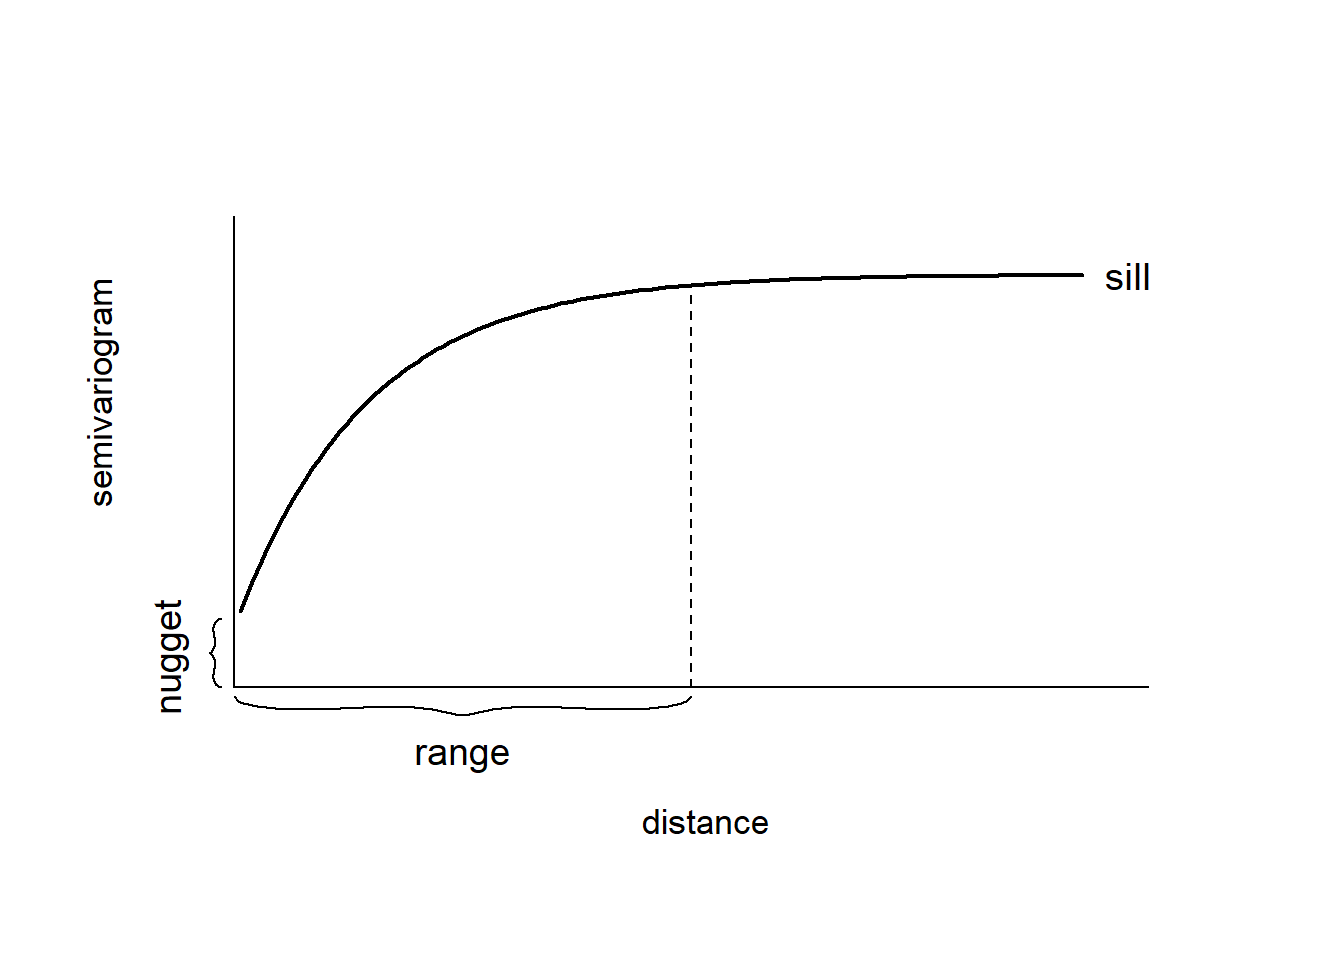
\includegraphics[width=0.85\textwidth]{typicalsemivariogram-1.png}
    \caption{A typical semivariogram}
    \label{fig:semivariogram}
\end{figure}
The empirical semivariogram is an exploratory tool useful for assessing whether data exhibit spatial correlation. Furthermore, it can be compared to a Monte Carlo envelope of empirical semivariograms calculated from random permutations of the data while keeping the locations fixed \autocite[][]{diggle2003introduction}. If the empirical semivariogram lies outside the Monte Carlo envelope with increasing distance, this is an indication of spatial correlation.\\
These graphs are again taken from "Geospatial Health Data: Modeling and Visualization with R-INLA and Shiny" by Paula Moraga \autocite[][]{moraga2019geospatial}. 
An example of a semivariogram is shown in Figure~\ref{fig:semivariogram}. This graph is taken from "Geospatial Health Data: Modeling and Visualization with R-INLA and Shiny" by Paula Moraga \autocite[][]{moraga2019geospatial}. \\ 
The dependence structure of a GRF is given by the covariance matrix, which is constructed from a covariance function. Matérn models and exponential functions are conventionally used for this purpose \autocite[][]{gelfand2010handbook}. For the locations $s_i, s_j\in\mathbb{R}^2$ the exponential covariance function is given by
\begin{equation}
\hbox{Cov}\left(Z\left(s_i\right), Z\left(s_j\right)\right)=\sigma^2\exp\left(-\kappa\left|\left|s_i-s_j\right|\right|\right),
\end{equation}
where the distance between the locations $s_i$ and $s_j$ is denoted by $\left|\left|s_i-s_j\right|\right|$, the variance of the spatial field is given by $\sigma^2$, while $\kappa>0$ controls the rate at which the correlation decays as the distance increases. \\
The Matérn family represents a flexible class of covariance functions that arises naturally in a variety of scientific fields \autocite[][]{guttorp2006studies}. The Matérn covariance function is written as
\begin{equation}
    \hbox{Cov}\left(Z\left(s_i\right),Z\left(s_j\right)\right)=\frac{\sigma^2}{2^{\nu-1}\Gamma\left(\nu\right)}\left(\kappa\left|\left|s_i-s_j\right|\right|\right)^{\nu}K_\nu\left(\kappa\left|\left|s_i-s_j\right|\right|\right).
\end{equation}
$\sigma^2$ denotes the marginal variance of the spatial field, $K_\nu\left(\cdot\right)$ represents the modified Bessel function of second kind and order $\nu>0$, where $\nu$ is an integer. The mean square differentiability of the process is determined by $\nu$ and is usually fixed since it is difficult to identify in applications. For $\nu=0.5$, this covariance function is the equivalent of the exponential covariance function. $\kappa > 0$ is related to the range $\rho$, which is defined as the distance at which there is approximately no correlation between two given points, $\rho=\sqrt{8\nu}/\kappa$ to be exact \autocite[][]{cameletti2013spatio}. Examples of these two covariance functions are shown in Figure~\ref{fig:covariance}. These graphs are again taken from "Geospatial Health Data: Modeling and Visualization with R-INLA and Shiny" by Paula Moraga \autocite[][]{moraga2019geospatial}. 
\begin{figure}[H]
    \centering
    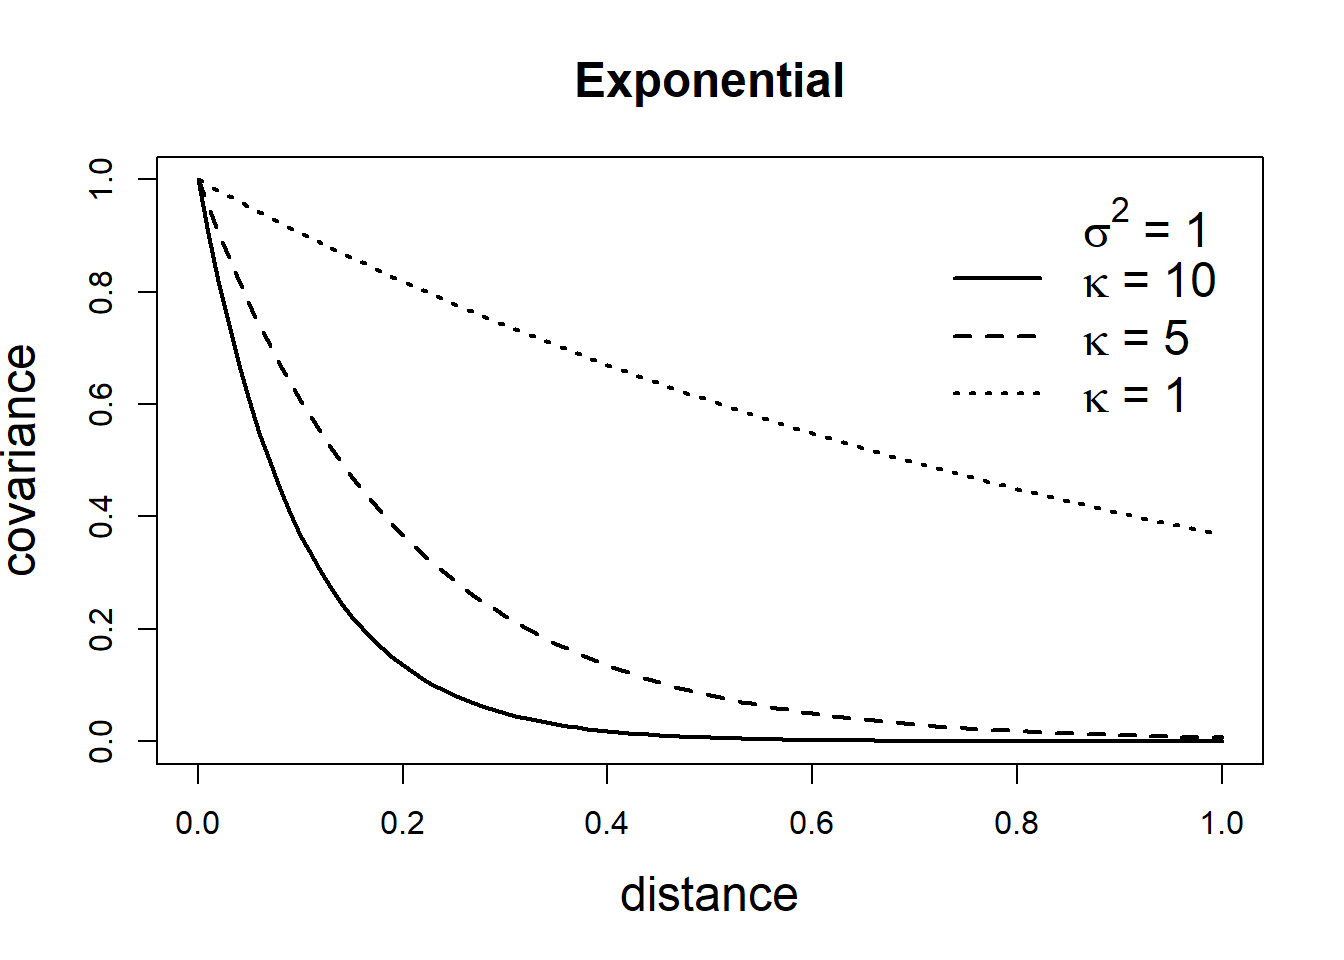
\includegraphics[width=0.8\textwidth]{covariancefunctions-1.png}
    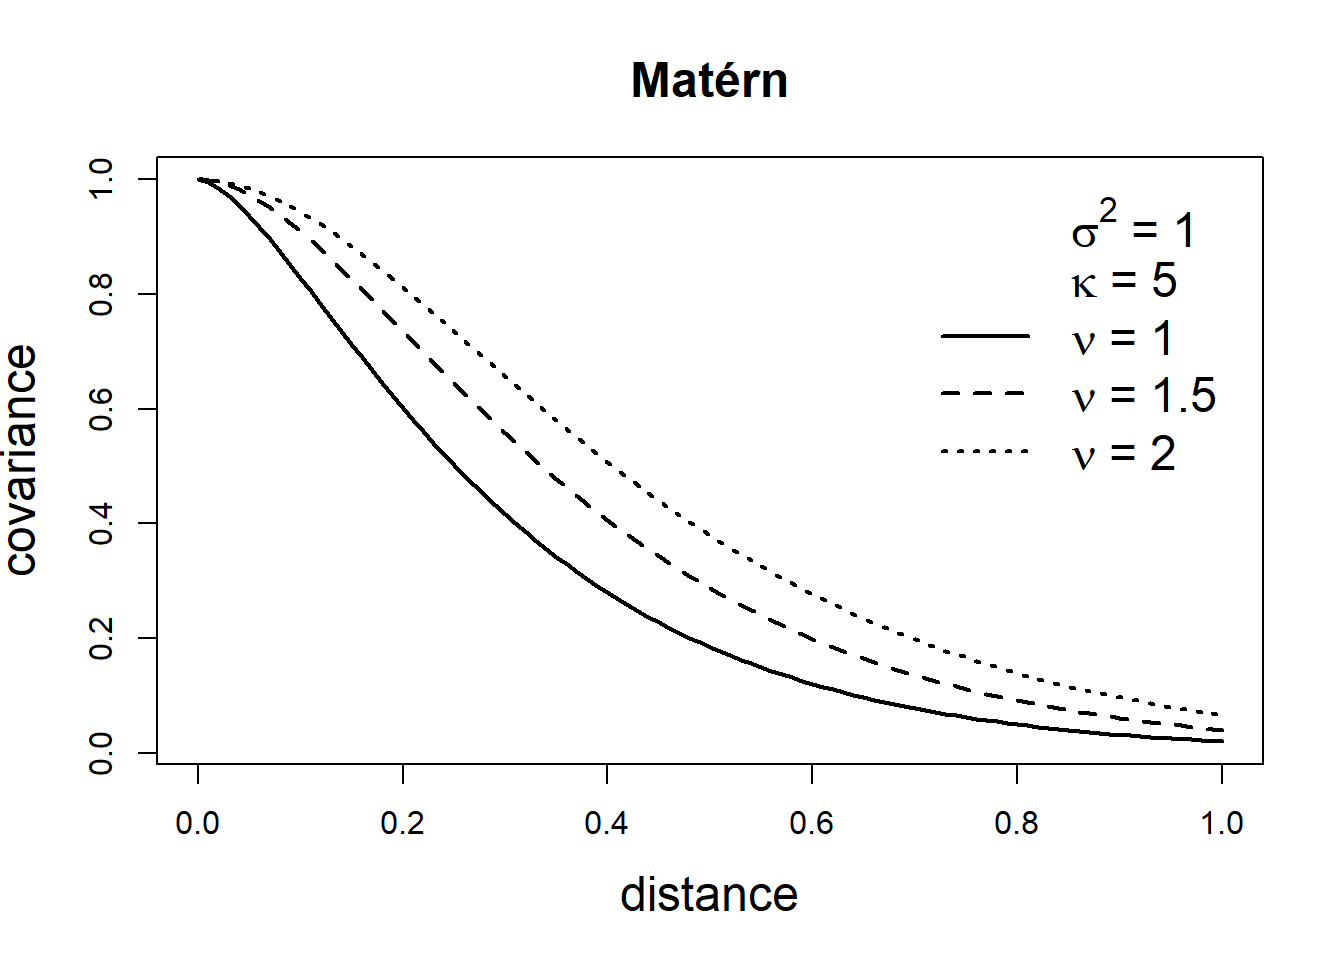
\includegraphics[width=0.8\textwidth]{covariancefunctions-2.png}
    \caption{Covariance functions corresponding to exponential and Matérn models.}
    \label{fig:covariance}
\end{figure}
\subsection{Gaussian Markov Random Fields}
\subsubsection{Definition of GMRFs}
Let $\pmb{x}=\left(x_1,...,x_n\right)^T$ be normally distributed with mean $\pmb{\mu}$ and covariance matrix $\pmb{\Sigma}$. Let $\mathcal{G}=\left(\mathcal{V}, \mathcal{E}\right)$, where $\mathcal{V}=\left\lbrace 1,...,\right\rbrace$ and $\mathcal{E}$ be such that there is no edge between nodes $i$ and $j$ exactly when $x_i\perp x_j|\pmb{x}_{ij}$. Then $\pmb{x}$ is a \textit{Gaussian Markov random field} (GMRF) with respect to $\mathcal{G}$. \\
Since $\pmb{\mu}$ does not affect the pairwise conditional independence properties of $\pmb{x}$, this information is 'hidden' in $\pmb{\Sigma}$. Hence,
\begin{equation*}
    x_i\perp x_j|x_{ij}\Longleftrightarrow Q_{ij}=0.
\end{equation*}
Therefore, the non-zero pattern of $\pmb{Q}$ determines $\mathcal{G}$, i.e. whether $x_i$ and $x_j$ are conditionally independent, and can be derived from $\pmb{Q}$. If $\pmb{Q}$ is a fully dense matrix, then $\mathcal{G}$ is fully connected, implying that any normal distribution with SPD covariance matrix is a GMRF and vice versa. \\
The elements of $\pmb{Q}$ are used for conditional interpretations. For any GMRF with respect to $\mathcal{G}=\left(\mathcal{V}, \mathcal{E}\right)$ with mean $\pmb{\mu}$ and precision matrix $\pmb{Q} > 0$,
\begin{align}
    \mathbb{E}\left[x_i|\pmb{x}_{-i}\right] &= \mu_i-\frac{1}{Q_{ii}}\sum_{j:j\sim i}Q_{ij}\left(x_j-\mu_j\right), \label{eq:mean_gmrf}\\
    \hbox{Prec}\left(x_i|\pmb{x}_{-i}\right) &= Q_{ii} \hspace{20pt}\hbox{ and }\label{eq:prec_gmrf}\\
    \hbox{Corr}\left(x_i,x_j|\pmb{x}_{ij}\right) &= -\frac{Q_{ij}}{\sqrt{Q_{ii}Q_{jj}}},\hspace{20pt} i\neq j
\end{align}
\autocite[][21]{rue2005gaussian}. \\
On the main diagonal of $\pmb{Q}$ are the conditional precisions of $x_i$ given $\pmb{x}_{-i}$ are placed, while the other elements, when scaled appropriately, provide information about the conditional correlation between $x_i$ and $x_j$ given $\pmb{x}_{ij}$. Since $\hbox{Var}\left(x_i\right)=\Sigma_{ii}$ and $\hbox{Corr}\left(x_i,x_j\right)=\Sigma_{ij}/\sqrt{\Sigma_{ii}\Sigma_{jj}}$, the information about the marginal variance of $x_i$ and the marginal correlation between $x_i$ and $x_j$ is given by $\pmb{\Sigma}$. The marginal interpretation provided by the correlation matrix is intuitive and informative, as the scope of the interpretation is reduced from an $n$-dimensional distribution to a one- or two-dimensional distribution. $\pmb{Q}$ is difficult to interpret marginally because either $\pmb{x}_{-i}$ or $\pmb{x}_{ij}$ would have to be integrated out of the joint distribution parameterized with respect to $\pmb{Q}$. $\pmb{Q}^{-1}=\pmb{\Sigma}$ by definition, and in general $\Sigma_{ii}$ depends on each element in $\pmb{Q}$ and vice versa \autocite[][20--23]{rue2005gaussian}.
\subsubsection{Markov Properties of GMRFs}
One property of GMRFs is that more information regarding conditional independence can be extracted from $\mathcal{G}$. The following three properties are equivalent. \\
The \textit{pairwise Markov property}:
\begin{equation*}
    x_i\perp x_j|\pmb{x}_{ij}\hspace{20pt}\hbox{ if }\left\lbrace i,j\right\rbrace\notin\mathcal{E}\hbox{ and }i\neq j.
\end{equation*}
The \textit{local Markov property}:
\begin{equation*}
    x_i\perp \pmb{x}_{-\left\lbrace i, \hbox{ne}\left(i\right)\right\rbrace}|\pmb{x}_{\hbox{ne}\left(i\right)}\hspace{20pt}\forall i\in\mathcal{V}.
\end{equation*}
The \textit{global Markov property}:
\begin{equation*}
    \pmb{x}_{A}\perp \pmb{x}_{B}|\pmb{x}_{C}
\end{equation*}
for all disjoint sets $A$, $B$ and $C$ where $A$ and $B$ are non-empty and separated by $C$. \\ Illustrations for these properties are shown in Figure~\ref{fig:pairwise}, Figure~\ref{fig:local} and Figure~\ref{fig:global}. These illustrations are taken from Rue and Held \autocite[][23--24]{rue2005gaussian}.
\begin{figure}[H]
    \centering
    \ctikzfig{ind_fig1}
    \caption{The pairwise Markov property; the black nodes are conditionally independent given the light gray nodes.}
    \label{fig:pairwise}
\end{figure}
\begin{figure}[H]
    \centering
    \ctikzfig{ind_fig2}
    \caption{The local Markov property; the black nodes and white nodes are conditionally independent given the dark gray nodes.}
    \label{fig:local}
\end{figure}
\begin{figure}[H]
    \centering
    \ctikzfig{ind_fig3}
    \caption{The global Markov property; the dark gray and light gray nodes are globally independent given the black nodes.}
    \label{fig:global}
\end{figure}
\subsubsection{Conditional Properties of GMRFs}
An essential result of GMRFs is the conditional distribution for a subset $\pmb{x}_a$ given $\pmb{x}_{-A}$. Here the canonical parameterisation proves useful, since by definition it can be easily updated by successive conditioning. \\
By splitting the indices into the non-empty sets A and B, of which the latter is equal to -A,
\begin{equation}\label{eq:partition_1}
    \pmb{x}=\begin{pmatrix}\pmb{x}_A\\\pmb{x}_B\end{pmatrix}.
\end{equation}
The mean and the precision are divided accordingly,
\begin{equation}\label{eq:partition_2}
    \pmb{\mu}=\begin{pmatrix}\pmb{\mu}_A\\\pmb{\mu}_B\end{pmatrix},\hspace{20pt}\hbox{ and }\hspace{20pt}\pmb{Q}=\begin{pmatrix}\pmb{Q}_{AA} & \pmb{Q}_{AB} \\ \pmb{Q}_{BA} & \pmb{Q}_{BB}\end{pmatrix}.
\end{equation}
The conditional distribution of $\pmb{x}_A|\pmb{x}_B$ is then a GMRF with respect to the subgraph $\mathcal{G}^A$ with mean $\pmb{\mu}_{A|B}$ and precision matrix $\pmb{Q}_{A|B}>0$, where
\begin{equation}
    \pmb{\mu}_{A|B}=\pmb{\mu}_A-\pmb{Q}_{AA}^{-1}\pmb{Q}_{AB}\left(\pmb{x}_B-\pmb{\mu}_B\right)
\end{equation}
and
\begin{equation*}
    \pmb{Q}_{A|B}=\pmb{Q}_{AA}.
\end{equation*}
Thus, the explicit knowledge of $\pmb{Q}_{A|B}$ is available through $\pmb{Q}_{AA}$, i.e. no calculation is required to obtain the conditional precision matrix. Moreover, the conditional mean depends only on the values of $\pmb{\mu}$ and $\pmb{Q}$ in $A\cup\,\hbox{ne}\left(A\right)$, since $Q_{ij} = 0\,\forall j\not in\hbox{ne}\left(i\right)$. \\
For successive conditioning, the canonical parameterisation for GMRF is useful. \\
A GMRF $\pmb{x}$ with respect to $\mathcal{G}$ and canonical parameters $\pmb{b}$ and $\pmb{Q}>0$ has the density
\begin{equation*}
    \pi\left(\pmb{x}\right)\propto\exp\left(-1\frac{1}{2}\pmb{x}^T\pmb{Q}\pmb{x}+\pmb{b}^T\pmb{x}\right).
\end{equation*}
The precision matrix is $\pmb{Q}$ and the mean is $\pmb{\mu}=\pmb{Q}^{-1}\pmb{b}$. The canonical parameterisation is written as 
\begin{equation*}
    \pmb{x}\sim \mathcal{N}_C\left(\pmb{b},\pmb{Q}\right).
\end{equation*}
Furthermore,
\begin{equation*}
    \mathcal{N}\left(\pmb{\mu},\pmb{Q}^{-1}\right) \Longleftrightarrow \mathcal{N}_C\left(\pmb{Q\mu}, \pmb{Q}\right).
\end{equation*}
If the indices are partitioned into two non-empty sets A and B and $\pmb{x}$, $\pmb{b}$ and $\pmb{Q}$ are partitioned as in \eqref{eq:partition_1} and \eqref{eq:partition_2}, then
\begin{equation}
    \pmb{x}_A|\pmb{x}_B\sim\mathcal{N}_C\left(\pmb{b}_A-\pmb{Q}_{AB}\pmb{x}_B,\pmb{Q}_{AA}\right).
\end{equation}
Let $\pmb{y}|\pmb{x}\sim\mathcal{N}\left(\pmb{x},\pmb{P}^{-1}\right)$ and $\pmb{x}\sim\mathcal{N}_C\left(\pmb{b},\pmb{Q}\right)$, then
\begin{equation}
    \pmb{x}|\pmb{y}\sim\mathcal{N}_C\left(\pmb{b}+\pmb{Py}, \pmb{Q}+\pmb{P}\right).
\end{equation}
This allows the calculation of conditional densities with multiple sources of conditioning, e.g. conditioning on observed data and a subset of variables. Therefore, the canonical parameterisation can be repeatedly updated without explicitly calculating the mean until it is actually needed. The computation of the mean requires the solution of $\pmb{Q\mu}=\pmb{b}$, but only matrix-vector products are needed for updating the canonical parameterisation \autocite[][25--27]{rue2005gaussian}.
\subsubsection{Specification Through Full Conditionals}
Alternatively, a GMRF can be specified by the full conditionals $\left\lbrace\pi\left(x_i|\pmb{x}_{-i}\right)\right\rbrace$ in place of $\pmb{\mu}$ and $\pmb{Q}$. Suppose the full conditionals are given as normals with
\begin{align}
    \mathbb{E}\left[x_i|\pmb{x}_{-i}\right] &= \mu_i-\sum_{j:j\sim i}\beta_{ij}\left(x_j-\mu_j\right)\hspace{20pt}\hbox{ and}\\
    \hbox{Prec}\left(x_i|\pmb{x}_{-i}\right) &= \kappa_i>0
\end{align}
for $i=1,...,n$, for $\pmb{\mu}$, $\pmb{\kappa}$ and some $\left\lbrace\eta_{ij},i\neq j\right\rbrace$. Evidently, $\sim$ is implicitly defined by the non-zero terms of $\left\lbrace\beta_{ij}\right\rbrace$. For there to exist a joint density $\pi\left(\pmb{x}\right)$ leading to these full conditional distributions, these full conditionals must be consistent. Since $\sim$ is symmetric, it follows that if $\beta_{ij}\neq 0$, then $\beta_{ji}\neq0$. If the entries of the precision matrix are chosen such that
\begin{equation*}
    Q_{ii}=\kappa_i, \hspace{20pt}\hbox{ and }\hspace{20pt} Q_{ij}=\kappa_i\beta_{ij}
\end{equation*}
and $\pmb{Q}$ must be symmetrical, i.e.,
\begin{equation*}
    \kappa_i\beta_{ij}=\kappa_j\beta_{ji},
\end{equation*}
then $\pmb{x}$ is a GMRF with respect to a labelled graph $\mathcal{G}=\left(\mathcal{V}, \mathcal{E}\right)$ with mean $\pmb{\mu}$ and precision matrix $\pmb{Q}=\left(Q_{ij}\right)$ \autocite[][27]{rue2005gaussian}.
\subsubsection{Multivariate GMRFs}
A \textit{multivariate GMRF} (MGMRF) is a multivariate extension of a GMRF that has proven useful in applications. Let $\pmb{x}$ be a GMRF with respect to $\mathcal{G}$, then the Markov property implies that
\begin{equation*}
    \pi\left(x_i|\pmb{x}_{-i}\right)=\pi\left(x_i|\left\lbrace x_j:j\sim i\right\rbrace\right).
\end{equation*}
$x_i$ is the value related to node $i$. Often the nodes have physical interpretations such as an administrative region of a country, which can be used to define the neighbours of node $i$. Let each of the $n$ nodes have an associated vector $\pmb{x}_i$ of dimension $p$, resulting in a GMRF of size $np$. Such a GMRF is denoted by $\pmb{x}=\left(\pmb{x}_1^T,...,\pmb{x}_n^T\right)^T$. The Markov property with respect to the nodes is preserved, i.e.,
\begin{equation*}
    \pi\left(\pmb{x}_i|\pmb{x}_{-i}\right)=\pi\left(\pmb{x}_i|\left\lbrace\pmb{x}_{j}:j\sim i\right\rbrace\right),
\end{equation*}
where $\sim$ is with respect to \textit{the same graph} $\mathcal{G}$. Let $\pmb{\mu}=\left(\pmb{\mu}_1^T,... ,\pmb{\mu}_n^T\right)^T$ be the mean of $\pmb{x}$, where $\mathbb{E}\left[\pmb{x}_i\right]=\pmb{\mu}_i$, and $\widetilde{\pmb{Q}}=\left(\widetilde{\pmb{Q}}_{ij}\right)$ its precision matrix, where each element of the matrix is a $p\times p$ matrix. \\
It follows that
\begin{equation*}
    \pmb{x}_i\perp\pmb{x}_j|\pmb{x}_{-ij}\Longleftrightarrow\widetilde{\pmb{Q}}_{ij}=\pmb{0}.
\end{equation*}
Formally, a random vector $\pmb{x}=\left(\pmb{x}_1^T,...,\pmb{x}_n^T\right)^T$ with $\dim\left(\pmb{x}_i\right)=p$, is called a $\hbox{MGMRF}_p$ with respect to $\mathcal{G}=\left(\mathcal{V}=\left\lbrace 1,. ...,n\right\rbrace,\mathcal{E}\right)$ with mean $\pmb{\mu}$ and precision matrix $\widetilde{\pmb{Q}} >0$, exactly when its density has the form
\begin{align*}
    \pi\left(\pmb{x}\right) &=\left(\frac{1}{2\pi}\right)^{np/2}\left|\widetilde{\pmb{Q}}\right|^{1/2}\exp\left(-\frac{1}{2}\left(\pmb{x}-\pmb{\mu}\right)^T\widetilde{\pmb{Q}}\left(\pmb{x}-\pmb{\mu}\right)\right)\\
    &=\left(\frac{1}{2}\right)^{np/2}\left|\widetilde{\pmb{Q}}\right|^{1/2}\exp\left(-\frac{1}{2}\sum_{ij}\left(\pmb{x}_i-\pmb{\mu}_i\right)^T\widetilde{\pmb{Q}}_{ij}\left(\pmb{x}_j-\pmb{\mu}_j\right)\right)
\end{align*}
and
\begin{equation*}
    \widetilde{\pmb{Q}}_{ij}\neq0\Longleftrightarrow\left\lbrace i,j\right\rbrace\in\mathcal{E}\,\forall\,i\neq j.
\end{equation*}
A $\hbox{MGMRF}_p$ is equivalent to a GMRF of dimension $np$ with identical mean vector and precision matrix.  Therefore, all results valid for a GMRF are also valid for a $\hbox{MGMRF}_p$, with modifications, since the graph for a $\hbox{MGMRF}_p$ has size $n$ and is defined with respect to $\left\lbrace\pmb{x}_i\right\rbrace$, while for a GMRF it has size $np$ and is defined with respect to $\left\lbrace x_i\right\rbrace$.  \\
The interpretation of $\widetilde{\pmb{Q}}_{ii}$ and $\widetilde{\pmb{Q}}_{ij}$ can be derived from the full conditional $\pi\left(\pmb{x}_i|\pmb{x}_{-i}\right)$. The extensions of \eqref{eq:mean_gmrf} and \eqref{eq:prec_gmrf} are
\begin{align}
    \mathbb{E}\left[\pmb{x}_i|\pmb{x}_{-i}\right]&=\pmb{\mu}_i-\widetilde{\pmb{Q}}_{ii}^{-1}\sum_{j:j\sim i}\widetilde{\pmb{Q}}_{ij}\left(\pmb{x}_j-\pmb{\mu}_j\right)\\
    \hbox{Prec}\left(\pmb{x}_i|\pmb{x}_{-i}\right) &= \widetilde{\pmb{Q}}_{ii}.
\end{align}
In some applications, the full conditionals
\begin{align}
    \mathbb{E}\left[\pmb{x}_i|\pmb{x}_{-i}\right] &= \pmb{\mu}_i-\sum_{j:j\sim i}\pmb{\beta}_{ij}\left(\pmb{x}_j-\pmb{\mu}_j\right) \\
    \hbox{Prec}\left(\pmb{x}_i|\pmb{x}_{-i}\right) &= \pmb{\kappa}_i > 0,
\end{align}
In some applications, the full conditionals are used to define the $\hbox{MGMRF}_p$, for given $p\times p$-matrices $\left\lbrace\pmb{\beta}_{ij},i\neq j\right\rbrace$, $\left\lbrace\pmb{\kappa}_i\right\rbrace$, and vectors $\pmb{\mu}_i$. Again, $\sim$ is implicitly defined by the non-zero matrices $\left\lbrace\pmb{\kappa}_i\right\rbrace$. Similar requirements as for $p=1$ apply to the existence of the joint density: $\pmb{\kappa}_i\pmb{\beta}_{ij}=\pmb{\beta}_{ij}^T\pmb{\kappa}_j$ for $i\neq j$ and $\widetilde{\pmb{Q}} > 0$. The $p\times p$ elements of $\widetilde{\pmb{Q}}$ are
\begin{equation*}
    \widetilde{\pmb{Q}}_{ij}=\begin{cases}
    \pmb{\kappa}_i\pmb{\beta}_{ij} & i\neq j \\
    \pmb{\kappa}_i & i=j
    \end{cases};
\end{equation*}
therefore $\widetilde{\pmb{Q}}>0\Longleftrightarrow\left(\pmb{I}+\left(\pmb{\beta}_{ij}\right)\right) > 0$ \autocite[][29--30]{rue2005gaussian}.
\subsection{Integrated Nested Laplace Approximation}
An alternative to MCMC methods that is both less computationally intensive and suitable for performing approximate Bayesian inference in latent Gaussian models is \textit{Integrated nested Laplace Approximation} (INLA). The basis of INLA is the use of a combination of analytical approximations and numerical algorithms for sparse matrices to approximate the posterior distribution using closed-form expressions. This speeds up inference and circumvents problems of sample convergence and mixing, making it suitable for fitting large data sets or exploring other models \autocite[][]{rue2009approximate}.  \\
INLA can be used for all models of the following form,
\begin{align*}
    y_i|\pmb{x},\pmb{\theta} &\sim \pi\left(y_i|x_i,\pmb{\theta}\right), \hspace{20pt} i=1,...,n,\\
    \pmb{x}|\pmb{\theta} &\sim \mathcal{N}\left(\mu\left(\pmb{\theta}\right), \pmb{Q}\left(\pmb{\theta}\right)^{-1}\right), \\
    \pmb{\theta} &\sim \pi\left(\pmb{\theta}\right).
\end{align*}
As introduced in \autoref{sec:notation}, $\pmb{y}$ are the observed data, $\pmb{x}$ is a Gaussian field, $\pmb{\theta}$ represents the hyperparameters, while $\mu\left(\pmb{\theta}\right)$ and $\pmb{Q}\left(\pmb{\theta}\right)$ denote the mean and precision matrix respectively. To ensure fast inference, the dimension of the hyperparameter vector $\pmb{\theta}$ should be small, since the approximations are computed by numerical integration over the hyperparameter space. \\
In most cases, the observations $y_i$ are assumed to belong to the exponential family with mean $\mu_i=g^{-1}\left(\eta_i\right)$. As shown in equation \eqref{eq:predictor}, $\eta_i$ accounts for the effects of several covariates in an additive way, which makes it suitable for a wide range of models, including spatial and spatio-temporal models, since $\left\lbrace f^{(j)}\right\rbrace$ can take very different forms. \\
Let $\pmb{x}=\left(\alpha,\left\lbrace\beta_k\right\rbrace|\theta\sim\mathcal{N}\left(\mu\left(\theta\right), \pmb{Q}\left(\theta\right)^{-1}\right)\right)$ be the vector of latent Gaussian variables, and let $\pmb{\theta}$ be the vector of hyperparameters, which are not required to be Gaussian. INLA calculates accurate and fast approximations for the posterior marginals of the components of the latent Gaussian variables
\begin{equation*}
    \pi\left(x_i|\pmb{y}\right),\hspace{20pt}i=1,...,n,
\end{equation*}
as well as the posterior marginals for the hyperparameters of the latent Gaussian model
\begin{equation*}
    \pi\left(\theta_j|\pmb{y}\right),\hspace{20pt}j=1,...,\dim\left(\pmb{\theta}\right).
\end{equation*}
For each element $x_i$ of $\pmb{x}$ the posterior marginals are given by
\begin{equation}
    \pi\left(x_i|\pmb{y}\right)=\int\pi\left(x_i|\pmb{\theta},\pmb{y}\right)\pi\left(\pmb{\theta}|\pmb{y}\right)d\pmb{\theta},
\end{equation}
and the posterior marginal for the hyperparameters can be expressed by
\begin{equation}
    \pi\left(\theta_j|\pmb{y}\right)=\int\pi\left(\pmb{\theta}|\pmb{y}\right)d\pmb{\theta}_{-j}.
\end{equation}
$\pi\left(x_i|\pmb{y}\right)$ is approximated by combining analytical approximations to the full conditionals $\pi\left(x_i|\pmb{\theta},\pmb{y}\right)$ and $\pi\left(\pmb{\theta}|\pmb{y}\right)$ and numerical integration routines to integrate out $\pmb{\theta}$. Similarly, $\pi\left(\theta_j|\pmb{y}\right)$ is approximated by approximating $\pi\left(\pmb{\theta}|\pmb{y}\right)$ and integrating out $\pmb{\theta}_{-j}$. In particular, the posterior density of $\pmb{\theta}$ is obtained through Gaussian approximation for the posterior of the latent field, $\widetilde{\pi}_G\left(\pmb{x}|\pmb{\theta},\pmb{y}\right)$, evaluated at the posterior mode, $x^*\left(\pmb{\theta}\right)=\arg\max_{\pmb{x}}\pi_G\left(\pmb{x}|\pmb{\theta},\pmb{y}\right)$,
\begin{equation}
    \widetilde{\pi}\left(\pmb{\theta}|\pmb{y}\right)\propto\frac{\pi\left(\pmb{x},\pmb{\theta},\pmb{y}\right)}{\widetilde{\pi}_G\left(\pmb{x}|\pmb{\theta},\pmb{y}\right)}\bigg|_{\pmb{x}=x^*\left(\pmb{\theta}\right)}.
\end{equation}
Next, the following nested approximations are constructed,
\begin{equation}
    \widetilde{\pi}\left(x_i|\pmb{y}\right)=\int\widetilde{\pi}\left(x_i|\pmb{\theta},\pmb{y}\right)\widetilde{\pi}\left(\pmb{\theta}|\pmb{y}\right)d\pmb{\theta},\hspace{20pt}\widetilde{\pi}\left(\theta_j|\pmb{y}\right)=\int\widetilde{\pi}\left(\pmb{\theta}|\pmb{y}\right)d\pmb{\theta}_{-j}.
\end{equation}
Finally, these approximations are numerically integrated with respect to $\pmb{\theta}$
\begin{align}
    \widetilde{\pi}\left(x_i|\pmb{y}\right)&=\sum_k\widetilde{\pi}\left(x_i|\theta_k,\pmb{y}\right)\widetilde{\pi}\left(\theta_k|\pmb{y}\right)\times\Delta_k,\\
    \widetilde{\pi}\left(\theta_j|\pmb{y}\right)&=\sum_l\widetilde{\pi}\left(\theta_l^*|\pmb{y}\right)\times\Delta_l^*,
\end{align}
with $\Delta_k$ and $\Delta_l^*$ representing the area weights corresponding to $\theta_k$ and $\theta_l^*$. \\
To obtain the approximations for the posterior marginals for the $x_i$'s conditioned on selected values of $\theta_k$ and $\widetilde{\pi}\left(x_i|\theta_k,\pmb{y}\right)$, a Gaussian, Laplace or simplified Laplace approximation can be used. Using a Gaussian approximation derived from $\widetilde{\pi}_G\left(\pmb{x}|\pmb{\theta},\pmb{y}\right)$ is the simplest and fastest solution, but in some situations it produces errors in the location and is unable to capture skewness behaviour. Therefore, the Laplace approximation is favoured over the Gaussian approximation, although it is relatively expensive. The simplified Laplace approximation is associated with lower costs and addresses inaccuracies of the Gaussian approximation in terms of location and skewness in a satisfactory manner \autocite[][]{moraga2019geospatial}.
\clearpage
\section{Bayesian Spatial Models}
In general, it can be assumed that areas in close proximity to each other have a more frequent burden of disease than areas that are further away from each other. By setting up a neighbourhood structure, this "proximity" can be defined. It is assumed that $i$ and $j$ are neighbours if they share a common boundary, denoted $i\sim j$. The set of neighbours of region $i$ is denoted by $\delta_i$ and its size is given by $n_{\delta_i}$.
\subsection{Besag Spatial Models}
\subsubsection{Besags' Improper Spatial Model}
A commonly used approach to modelling spatial correlation is the Besag model, also known as an intrinsic GMRF model. The conditional distribution for a random vector $\pmb{x}=\left(x_1,...,x_n\right)^T$ is given by
\begin{equation}
    x_i|\pmb{x}_{-i},\tau_x\sim\mathcal{N}\left(\frac{1}{n_{\delta_i}}\sum_{j\in\delta_i}x_j,\frac{1}{n_{\delta_i}\tau_x}\right),
\end{equation}
with $\tau_x$ as a precision parameter. The mean of the effects over all neighbours is given by the mean of $x_i$, while the precision is proportional to the number of neighbours. The joint distribution for $\pmb{x}$ is given by
\begin{equation}
    \pi\left(\pmb{x}|\tau_x\right)\propto\exp\left(-\frac{\tau_x}{2}\sum_{i\sim j}\left(x_i-x_j\right)^2\right)\propto\exp\left(-\frac{\tau_x}{2}\pmb{x}^T\pmb{Q}\pmb{x}\right).
\end{equation}
The precision matrix $\pmb{Q}$ is given by
\begin{equation}
    Q_{ij}=\begin{cases}
    n_{\delta_i}&i=j,\\
    -1&i\sim j,\\
    0&\hbox{else.}
    \end{cases}
\end{equation}
\pmb{Q} is a singular matrix, i.e. it has a non-empty null space $\pmb{V}$, hence the model is called intrinsic or Besags' improper spatial model. \\
The Besag model for spatial effects has one hyperparameter, the precision $\tau_x$, which is represented as
\begin{equation}
    \theta_1 = \log\tau_x.
\end{equation}
The prior is defined on $\theta_1$ \autocite[][]{besag1974spatial, riebler2016intuitive}.
\subsubsection{Besags' Proper Spatial Model}
To overcome this impropriety, the precision matrix has to be redefined as follows,
\begin{equation}
    Q_{ij} = \begin{cases}
    \tau_x\left(n_{\delta_i}+d\right) & i=j,\\
    -\tau &\hbox{else.}
    \end{cases}
\end{equation}
$d > 0$  is an additional term added to the diagonal to control the "properness". The conditional distribution for the proper version of the Besag model is then given by
\begin{equation}
    x_i|\pmb{x}_{-i},\tau_x,d\sim\mathcal{N}\left(\frac{1}{d+n_{\delta_i}}\sum_{i\sim j}x_j\frac{1}{\tau_x\left(d+n_{\delta_i}\right)}\right).
\end{equation}
The proper version of the Besag model for spatial effects has two hyperparameters, the precision $\tau_x$, which is represented as
\begin{equation}
    \theta_1 = \log\tau_x
\end{equation}
and the diagonal parameter $d$, which is represented as
\begin{equation}
    \theta_2 = \log d.
\end{equation}
The priors are defined on $\theta_1$ and $\theta_2$, respectively \autocite[][]{besag1974spatial, riebler2016intuitive}.
\subsection{The Besag-York-Mollié Model}
The Besag-York-Mollié (BYM) model is a lognormal Poisson model that is a combination of a Besag model $u$ and an ordinary random effect component $v$ for non-spatial heterogeneity. It combines the regional spatial effect $\pmb{x}$ into the sum of an unstructured and a structured spatial component, so that $\pmb{x}=\pmb{v}+\pmb{u}$.\\
$\pmb{v}\sim\mathcal{N}\left(0,\tau_v^{-1}\pmb{I}\right)$ accounts for pure overdispersion, while $\pmb{u}\sim\mathcal{N}\left(\pmb{0}, \tau_u^{-1}\pmb{Q}^{-}\right)$ is the Besag model. \\
By using a spatial and a non-spatial error term, the overdispersion that is not modelled by the Poisson variables is taken into account. Thus, if the observed variance is not fully explained by the spatial structure of the data, the error terms explain the rest of the variance. \\
The resulting covariance matrix of $\pmb{x}$ is given by
\begin{equation}
    \hbox{Var}\left(\pmb{x}|\tau_u,\tau_v\right)=\tau_v^{-1}\pmb{I}+\tau_u^{-1}\pmb{Q}^{-},
\end{equation}
where $\pmb{Q}^{-}$ denotes the generalised inverse of \pmb{Q}. \\
The hyperparameters of the model are the precision $\tau_u$ of the Besag model $u$ and the precision $\tau_v$ of the iid model $v$. They are represented as
\begin{equation}
    \pmb{\theta}=\left(\theta_1, \theta_2\right)=\left(\log\tau_v,\log\tau_u\right)
\end{equation}
and the prior is defined on $\pmb{\theta}$ \autocite[][]{besag1991bayesian, riebler2016intuitive}.
\subsection{The Leroux Model}
One problem with the BYM model is that the structured and unstructured components are not identifiable because they cannot be considered independently. Moreover, $\tau_v$ and $\tau_u$ do not represent variability at the same level, which makes the choice of hyperpriorities difficult. The Leroux model is formulated in such a way that the compromise between the two variations is made more explicit. It is assumed that $\pmb{x}$ follows a normal distribution with zero mean and covariance matrix
\begin{equation}
    \hbox{Var}\left(\pmb{x}|\tau_x,\phi\right)=\tau_x^{-1}\left(\left(1-\phi\right)\pmb{I}+\phi\pmb{Q}\right)^{-1},
\end{equation}
with $\phi\in\left[0,1\right]$ as mixing parameter. For $\phi=0$ the model reduces to pure overdispersion and for $\phi=1$ to the Besag model. The conditional expected value of $x_i$ for all other random effects is the weighted mean of the unstructured model with zero mean and the mean of the Besag model, while the conditional variance is the weighted mean of $\tau_x^{-1}$ and $\left(\tau_x\cdot\ n_{\delta_i}\right)^{-1}$ \autocite[][]{leroux2000estimation, riebler2016intuitive}.
\subsection{The BYM2 Model}
One problem that all the aforementioned models have is the lack of scaling of the spatially structured component. Scaling facilitates the assignment of hyperpriorities and ensures that the interpretation of hyperpriorities remains the same across different areas. \\
Since the Besag model penalises a local deviation from its null space, the hyperprior will control this local deviation and thus affect the smoothness of the estimated spatial effects. If the estimate of the field is too smooth, the precision will be large and the spatial variation may be blurred. On the other hand, if the precision is too small, the model could overfit due to the large local variability. \\
The marginal variances $\tau_x^{-1}\left[\pmb{Q}^{-}\right]_{ii}$ depend on the structure of the graph, which is reflected in the structure matrix $\pmb{Q}$. A generalised variance can be calculated as the geometric mean of the marginal variance as follows
\begin{equation}\label{eq:bym_scale}
    \sigma_{\hbox{GV}}^2\left(\pmb{u}\right)=\exp\left(\frac{1}{n}\sum_{i=1}^n\log\left(\frac{1}{\tau_x}\left[\pmb{Q}^{-}\right]_{ii}\right)\right)=\frac{1}{\tau_x}\exp\left(\frac{1}{n}\sum_{i=1}^n\log\left(\left[\pmb{Q}^{-}\right]_{ii}\right)\right).
\end{equation}
In order to unify the interpretation of a chosen prior for $\tau_x$ and make it transferable across domains, the structured effect must be scaled such that $\sigma_{\hbox{GV}}^2\left(\pmb{x}\right)=\tau_x^{-1}$. This implies that $\tau_x$ denotes the accuracy of the (marginal) deviation from a constant level, independent of the underlying graph. \\
A modification of the BYM model that addresses this scaling problem is the BYM2 model. It uses a scaled structured component $\pmb{u}_{*}$, where $\pmb{Q}_{*}$ denotes the precision matrix of the Besag model, scaled with the marginal variance $\sigma_{\hbox{GV}}^2$ as a factor. The random effect is then given by
\begin{equation}\label{eq:bym2_1}
    \pmb{x}=\frac{1}{\tau_x}\left(\sqrt{1-\phi}\pmb{v}+\sqrt{\phi}\pmb{u}_{*}\right),
\end{equation}
with covariance matrix
\begin{equation}
    \hbox{Var}\left(\pmb{x}|\tau_x,\phi\right)=\frac{1}{\tau_x}\left(\left(1-\phi\right)\pmb{I}+\phi\pmb{Q}_{*}^{-}\right).
\end{equation}
Equation~\ref{eq:bym2_1} emphasises the trade-off between pure overdispersion and spatially structured correlation, where $0\leq\phi\leq1$ measures the fraction of the marginal variance explained by the structured effect. For $\phi=0$ the model reduces to pure overdispersion, while for $\phi=1$ it becomes a Besag model \autocite[][]{martins2014penalising, riebler2016intuitive}.
\clearpage
\section{Goodness-of-Fit indicators}\label{sec:performance}
The goodness of fit indicates "how well" an estimated model can explain a set of observations. Measures of goodness of fit allow a statement to be made about the discrepancy between the theoretical values of the random variables under investigation, which are expected or predicted on the basis of the model, and the values actually measured. \\
The goodness of fit of a model to available data can be assessed with the help of statistical tests or suitable ratios.
\subsection{The Akaike Information Criterion}
The historically oldest criterion was proposed in 1973 by Hirotsugu Akaike (1927-2009) as an information criterion and is known today as the Akaike information criterion (AIC). The AIC is one of the most frequently used criteria for model selection in the context of likelihood-based inference.  \\
Let the population contain the distribution of a variable with unknown density function $p$. The maximum likelihood estimation assumes a known distribution with an unknown parameter $\theta$, hence the density function can be written as $q\left(\theta\right)$. The Kullback-Leibler divergence is used as a distance measure between $p$ and $q\left(\widehat{\theta}\right)$ with $\widehat{\theta}$ the estimated parameter from the maximum likelihood estimation. The better the maximum likelihood model, the small the Kullback-Leibler divergence $D\left(P||Q\right)$. \\
For a maximum likelihood model with a $p$-dimensional parameter vector $\widehat{\pmb{\theta}}$, the Akaike information criterion is defined as
\begin{equation}
    \hbox{AIC}=-2l\left(\widehat{\pmb{\theta}}_{ML}\right)+2p,
\end{equation}
with $l$ the log-likelihood function \autocite[][]{akaike1974new}.
\subsection{The Deviance Information Criterion}
In statistics, the deviance information criterion, or DIC for short, is a measure (criterion) for the prediction error of a model.
This measure is an information criterion and belongs to the environment of the Bayesian method for model comparisons. The smaller the deviance information criterion, the better the model fit. The deviance information criterion can be regarded as the Bayesian equivalent of the Akaike information criterion. \\
The deviance is defined as 
\begin{equation}
    D\left(\pmb{\theta}\right)=-2\log\left(l\left(\pmb{y}|\pmb{\theta}\right)\right)+C,
\end{equation}
with $\pmb{y}$ the data, $\pmb{\theta}$ the unknown parameters of the model and l the likelihood function. $C$ is a constant that cancels out in all calculations that compare different models and therefore it does not need to be known \autocite[][]{nelder1972generalized}. \\
The DIC is given by
\begin{equation}
    \hbox{DIC}=D\left(\overline{\pmb{\theta}}\right)+2p_D,
\end{equation}
with
\begin{equation}
    p_D=\overline{D\left(\pmb{\theta}\right)}-D\left(\overline{\pmb{\theta}}\right),
\end{equation}
where $\overline{\pmb{\theta}}$ is the expected value of $\pmb{\theta}$ \autocite[][]{spiegelhalter2014deviance}.
\subsection{The Watanabe-Akaike Information Criterion}
The Watanabe-Akaike information criterion (WAIC) is the generalised AIC onto singular statistical models. \\
The WAIC is given by
\begin{equation}
    \hbox{WAIC} = -2\hbox{LLPD}+2p_{\hbox{WAIC}},
\end{equation}
with the log pointwise predictive density (LLPD) given by
\begin{equation}
    \hbox{LLPD} = \sum_{i=1}^n\log\left(\int \pi\left(y_i|\pmb{\theta}\right)\pi_{\hbox{post}}\left(\pmb{\theta}\right)\right)d\pmb{\theta}.
\end{equation}
LLPD can be seen as the Bayesian analogue of $l\left(\widehat{\pmb{\theta}}_{ML}\right)$ in the calculation of the AIC.\\
The penalty term of the WAIC is also fully Bayesian and given by
\begin{equation}
    p_{\hbox{WAIC}}=\sum_{i=1}^n\hbox{Var}_{\hbox{post}}\left(\log\left(\pi\left(y_i|\pmb{\theta}\right)\right)\right),
\end{equation}
where the term represents the variance of the individual terms in the LLPD over all data points \autocite[][]{watanabe2010asymptotic, yong2018loo}.
\subsection{The Conditional Predictive Ordinate}
The conditional predictive ordinate (CPO) is a Bayesian diagnostic that can be used to detect surprising observations. It is often used in the context of univariate sampling, the multivariate normal distribution and regression models. \\
The conditional predictive ordinate is given by
\begin{equation}
    \hbox{CPO} = \pi\left(y_i|\pmb{y}_{-i}\right)
\end{equation}
with $\pmb{y}$ the data, $\pmb{y}_{-i}$ the data without the $i$-th observation, and $\pi\left(\cdot|\pmb{y}_{-i}\right)$ the predictive distribution of a new observation at $\pmb{y}_{-i}$. Low values of CPO are an indication that $y_i$ is surprising given prior knowledge and the other observations \autocite[][]{pettit1990conditional, cox1980discussion}.
\clearpage
\section{Model Issues}\label{sec:issues}
One problem that plagues these models is that they cannot be directly compared due to their different parameterisations and the fact that the precision in these models is interpreted differently. Since neither a Besag model nor a BYM model nor a Leroux model is scaled, the precision parameter is not representative of the marginal precision but is confounded with the mixing parameter. Therefore, the effect of a prior assigned to the precision parameter is dependent on the graph structure of the application. Thus, a given prior is not transferable between different applications if the underlying graph changes. Furthermore, the goal of the BYM2 model is not to optimise goodness-of-fit indicators, but to provide a meaningful model formulation where all parameters have a clear meaning. By mapping the precision parameter to the marginal standard deviation, the model parameters are flexible and the assignment of meaningful hyperpriorities is made easier \autocite[][]{riebler2016intuitive}. \\
Additionally, the goodness-of-fit indicators introduced in section~\ref{sec:performance} have their own problems. The DIC, for example, produces unreasonable results if the posterior distribution is not well summarised by its mean, while the WAIC is based on a data partition that would create difficulties for structured models, such as for spatial or network data \autocite[][]{gelman2014understanding}. \\
Finally, the choice of the prior also affects the value of these criteria and depending on the values chosen for the PC priors used in this work, overfitting of the models may occur, which is then reflected in these criteria, but more on this later.
\clearpage
\section{The Variance Inflation Factor}\label{sec:vif}
The Variance Inflation Factor ($\hbox{VIF}$) is a measurement that can be used to avoid multicollinearity between covariates. The $\hbox{VIF}$ quantifies the severity of multicollinearity in a generalised linear model. It provides an index that measures the extent to which the variance of an estimated regression coefficient is increased due to collinearity. \\
For $p-1$ independent variables, 
\begin{equation}
    \hbox{VIF}_i = \frac{1}{1-R^2},\hspace{20pt}i=1,...,p-1,
\end{equation}
with $R^2$ the coefficient of determination. In most literature, a value of at least 5 is suggested as too high and is therefore used as the threshold in this work \autocite[][]{craney2002model}.
\clearpage
\section{Calculation of the Mean and Quantiles}\label{sec:mean_iv}
As the posterior mean and the credibility intervals of coefficient are of interest, calculation of these is performed later on. This allows a better interpretation of the results. \\
To compute the posterior mean of the coefficients, the code shown in Listing~\ref{codePosteriorMean} can be used. \\
To get the expected value given a marginal function $\pi\left(x\right)$, the expected value of a function $f\left(x\right)$ is calculated, i.e.
\begin{equation}
    \int f\left(x\right)\pi\left(x\right)dx.
\end{equation}
If necessary, e.g. if the target variable follows a (negative) binomial distribution, the value must be transformed to its original scale, as in these cases the log-likelihood is modelled. Therefore, in these cases, the expected value would have to be exponentiated to allow a clear interpretation. \\
To obtain a credibility interval of the fixed effects on the transformed scale, the code in Listing~\ref{codeCredibility} can be used. In practice, the marginals are first transformed to their original scale, if necessary, and then the 2.5\% quantile and the 97.5\% quantiles are calculated.
%https://arxiv.org/pdf/1708.02723.pdf \\
%http://www.leg.ufpr.br/~elias/cursos/br2019/slides1.pdf
% !TEX root = ../my-thesis.tex
%

\chapter{Analysis of Geospatial Health Data}
\label{sec:geodata}
Healthcare data provides information for detecting public health problems and reacting adequately when they occur. With this information, prevention and control of a multitude of health conditions including infectious diseases, non-communicable diseases, injuries and health-related behaviours can be achieved. To analyse and interpret health data, the process involves a wide variety of system designs, analytical methods, modes of presentation and interpretive uses\autocite[][]{teutsch2000principles}. Descriptive methods generally form the basis of routine reporting of surveillance data. Rather than focusing on observed patterns in the data, these may also attempt to compare the relative occurrence of health outcomes in different subgroups. More specific hypotheses can be explored using inferential methods. The aim of these methods is to draw statistical inferences about patterns or outcomes of health. \\
The increasing availability of geo-referenced health data, population data, satellite imagery of environmental factors influencing levels of disease activity, and the development of geographic information systems (GIS) and address geocoding software, the rise of studies of spatial and spatio-temporal variation in disease has been facilitated. \\
A broad range of spatial and spatio-temporal methods exist for disease surveillance, including methods for disease mapping, clustering and geographic correlation studies. These methods can be used to identify areas of high risk, risk factors, evaluate spatial variations in temporal trends, measure excess disease risk near a suspected source and detect outbreaks at an early stage.
\clearpage
\section{Geographic Data}
In spatial statistics, two fundamental types of geographic data exist, namely \textit{vector data} and \textit{raster data}. In the vector data model, the world is represented by points, lines and polygons with discrete, well-defined boundaries, which tends to result in high accuracy. Raster data, on the other hand, divides the surface into cells of uniform size, and raster datasets are used as the basis for background images in web mapping. \\
Determining which data type to use depends on the domain of the application. Vector data dominates in the social sciences because human settlements typically have discrete boundaries, while raster data are commonly used in many environmental sciences because they are based on remote sensing data. Naturally, there is also some overlap and both types can be used together or one form can be converted into the other \autocite[][]{lovelace2019geocomputation}.
\subsection{Vector Data}
The geographic vector data model is based on points located within a \textit{coordinate reference system} (CRS), in which points either represent self-standing features or form more complex geometric shapes, i.e. lines and polygons. Using this system, Trondheim can be represented by the coordinates $\left(10.4, 63.4\right)$, meaning $10.4$ degrees east of the prime meridian and $63.4$ degrees north of the equator. It could also be written as $\left(1157722.70, 9199010.75\right)$, which is the position of Trondheim using the Web Mercator projection, the de facto standard for web mapping applications. More will be said about CRS later, but for now it is sufficient to know that it is possible to display coordinates in various ways. An example of a CRS is shown in Figure~\ref{fig:globe}.
\begin{figure}[H]
   \centering
       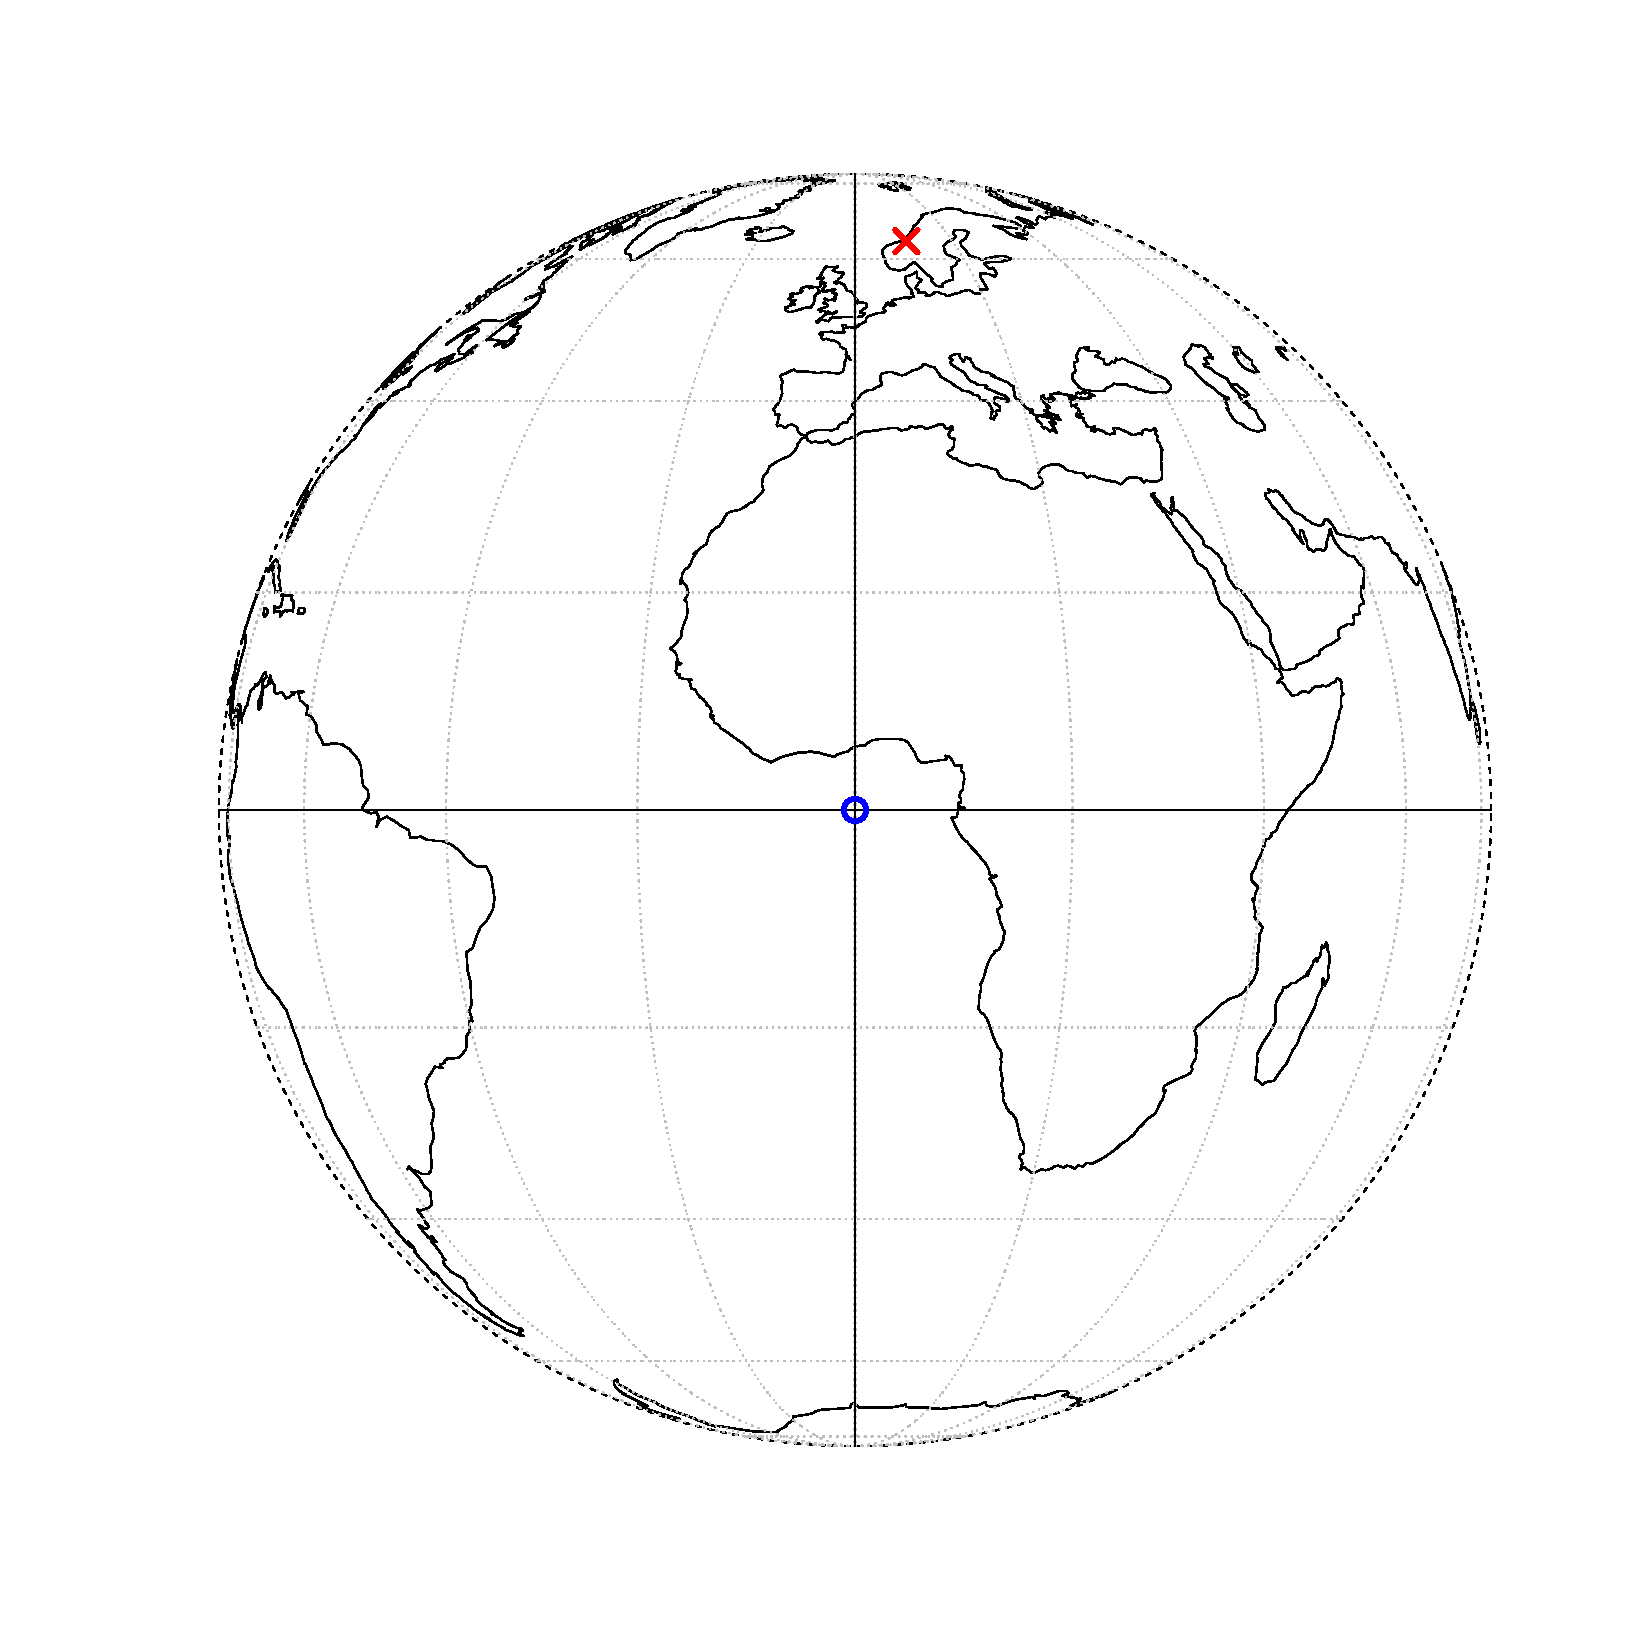
\includegraphics[page=1,width=.7\textwidth]{globe.pdf}
 \caption{A geographic CRS with an origin at 0° longitude and latitude. The red X denotes the location of Trondheim.}
 \label{fig:globe}
\end{figure}
\subsubsection*{Different Types of Vector Data}
As mentioned earlier, there are different types of vector data. There are 17 different geometry types in the standard \textit{simple features}, but there are seven core types that can be used in most analysis software. These types are visualised in Figure~\ref{fig:sf}.
\begin{figure}[H]
   \centering
       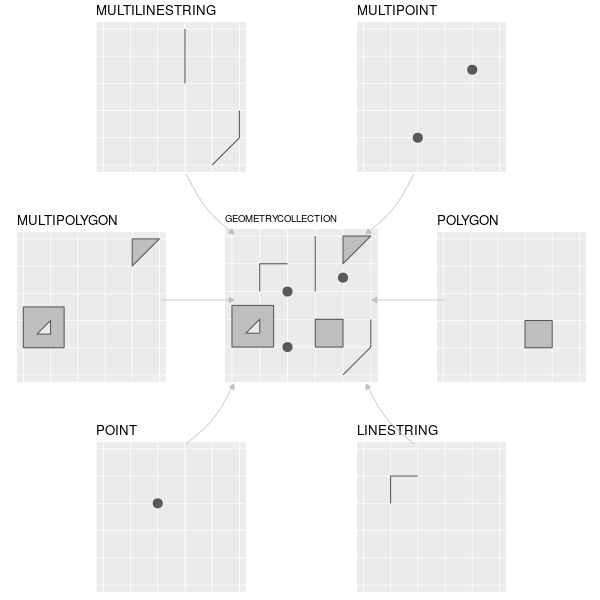
\includegraphics[width=.7\textwidth]{sf-classes.png}
 \caption{The most commonly used simple feature types.}
 \label{fig:sf}
\end{figure} $\newline$
Simple Features was developed by the Open Geospatial Consortium and is an open, standardised, hierarchical data model that represents a wide range of geometry types. The use of this data model ensures that scientific work can be transferred to other institutions, e.g. when importing from and exporting to spatial databases \autocite[][]{lovelace2019geocomputation}. 
\subsection{Raster Data}
The geographic raster data model consists in most cases of a raster header and a matrix representing uniformly distributed cells/pixels. The raster header defines the CRS, the origin (starting point) and the extent. Since the number of columns and rows and the resolution of the cell size are stored in the extent, starting from the origin, it is easy to access and change each cell by its ID or by specifying the row and column number. In this type of representation, the coordinates of the four vertices of each cell are not explicitly stored, instead only the origin is stored. This speeds up data processing and makes it more efficient, but each raster layer can only contain a single value, which can be either numeric or categorical. Typically, raster maps are used to depict continuous features such as elevation or temperature, but categorical variables, for example soil or land cover, as shown in Figure~\ref{fig:raster} \autocite[][]{lovelace2019geocomputation}.
\begin{figure}[H]
   \centering
       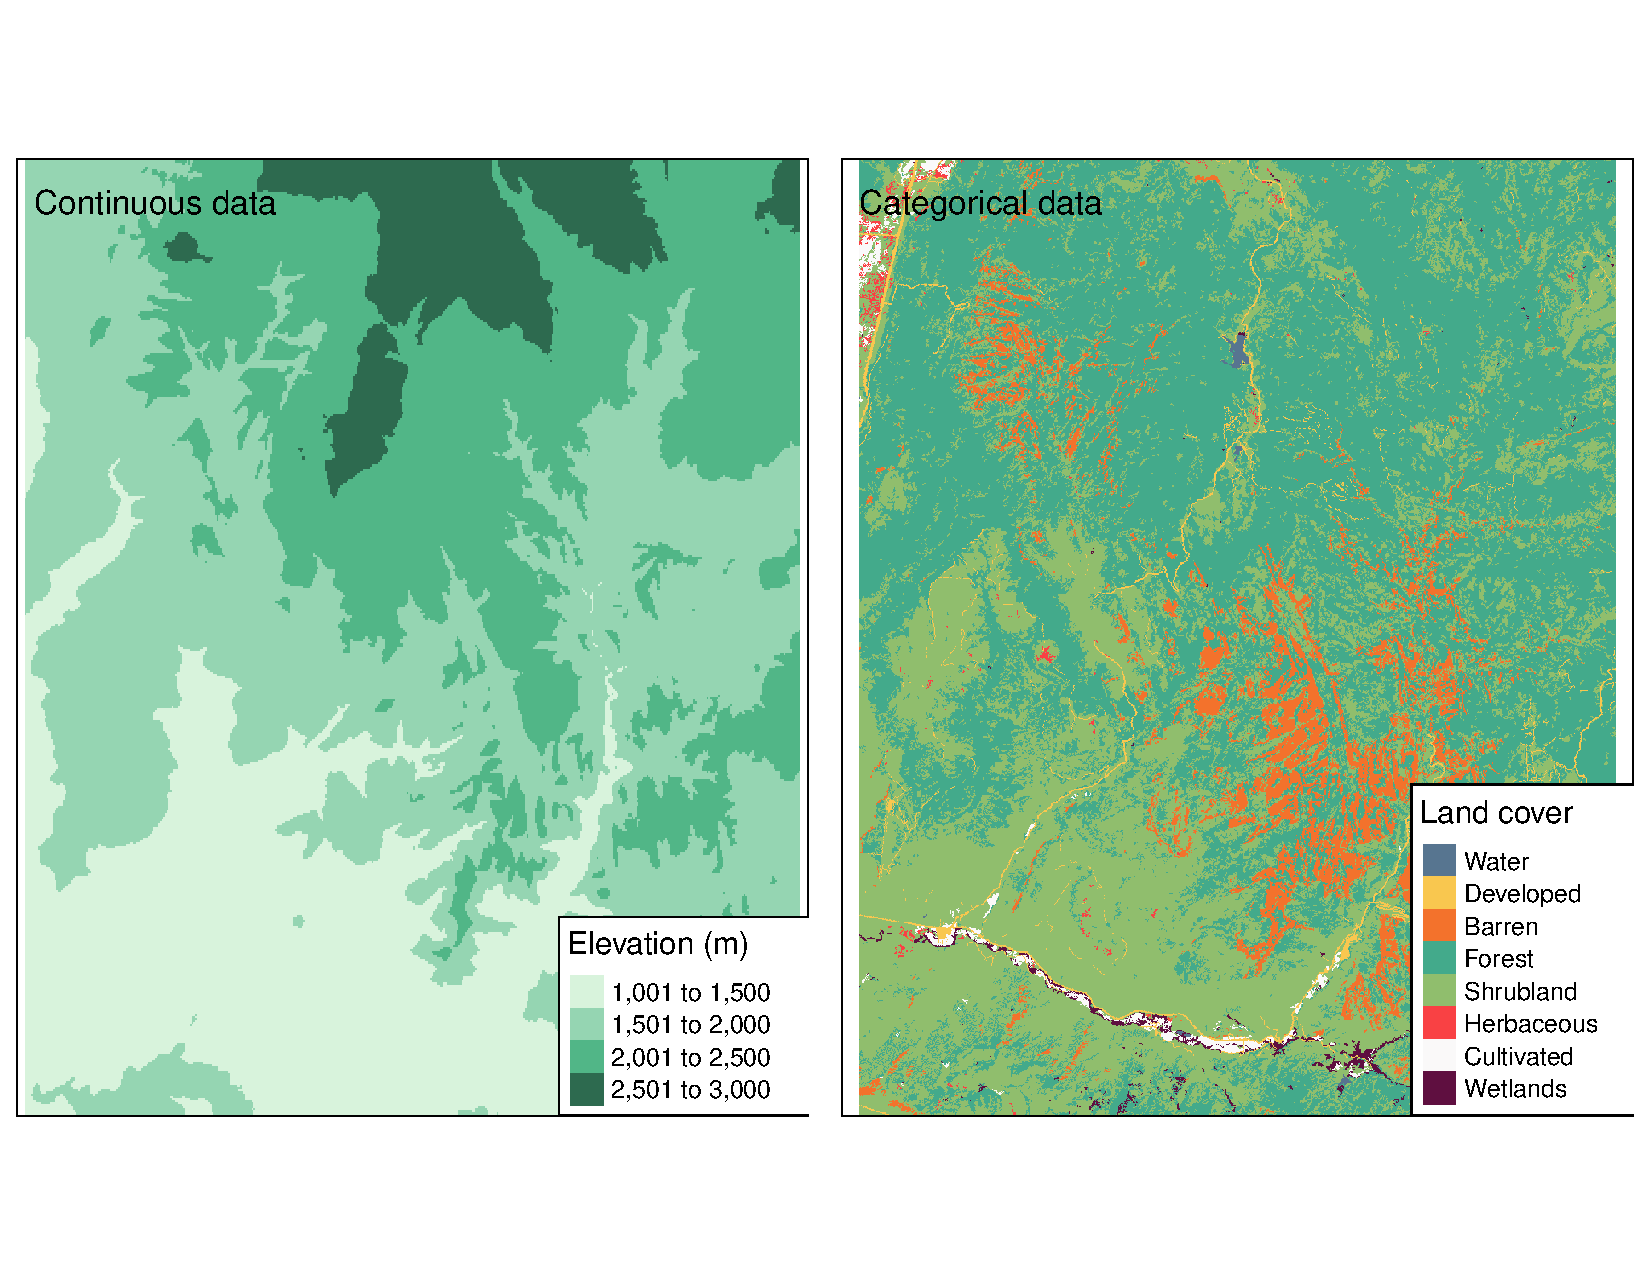
\includegraphics[page=1,width=\textwidth]{raster.pdf}
 \caption{An example of continuous and categorical raster data}
 \label{fig:raster}
\end{figure}
\subsection*{Coordinate Reference Systems}
A common denominator of vector and raster data are that both use the coordinate reference system (CRS), which defines how spatial elements relate to the surface of the Earth. The CRS can be either geographic or projected.
\subsubsection*{Geographic Coordinate Systems}
Geographic coordinate systems use two values, \textit{longitude} and \textit{latitude}, to identify any location on Earth. Longitude is defined as the east-west location at an angular distance from the prime meridian plane, while latitude is the angular distance north or south of the equator. Consequently, distances in geographic CRS are not measured in metres. \\
The Earth's surface is typically represented in geographical coordinate systems by a spherical or ellipsoidal surface. The former assumes that the Earth is a perfect sphere of a certain radius, which has the advantage of being a simplistic model, but is associated with inaccuracies owing to the fact that the Earth is not a sphere. Ellipsoidal models are defined by the equatorial radius and the polar radius, providing a better model since the equatorial radius is approximately 11.5 km longer than the polar radius.\\
The \textit{datum} is a broader component of CRS that contains information about which ellipsoid to use and the exact relationship between Cartesian coordinates and the location on the Earth's surface. The notation \textit{proj4string} is used to store these additional details. It allows for local variations of the Earth's surface, such as large mountain ranges, to be taken into account in local CRS. Datum can again be divided into two categories, \textit{local} and \textit{geocentric}, the difference being that in the local datum the ellipsoidal surface is shifted to match the surface at a particular location, whereas in the geocentric datum the centre of gravity of the Earth is the centre and the accuracy of the projections is not optimised for any particular location \autocite[][]{lovelace2019geocomputation}.
\subsubsection*{Projected Coordinate Systems}
Projected CRS are based on Cartesian coordinates on an implicitly flat surface and have an origin, $x$ and $y$ axes, and a linear unit of measurement, metres for instance. They are based on geographic CRS and rely on map projections to convert between the three-dimensional surface of the Earth and the east/north values ($x$ and $y$) in a projected CRS.\\
This transition always entails some distortion, skewing some of the properties of the earth's surface, such as area, direction, distance and shape. Generally, the name of a projection is based on a property it preserves, e.g. equal area projection preserves area, equidistant projection preserves distance and conformal projection preserves local shape. \\
Again, subgroups exist in projection coordinate systems, \textit{conic}, \textit{cylindrical} and \textit{planar} projections. In a conic projection, the earth's surface is projected onto a cone along one or two tangent lines. Along these lines the distortions are minimised and increase with the distance to the lines. The projection is therefore best suited for maps of mid-latitude areas. Cylindrical projections map the surface onto a cylinder. These types of projections can be created by touching the surface of the Earth along one or two tangent lines. They are often used to map the entire Earth. A planar projection projects data onto a flat surface that touches the globe at a point or along a tangent line, and is typically used in mapping polar projections \autocite[][]{lovelace2019geocomputation}.
\clearpage
% \section{Spatial Point Processes}
% A stochastic process that describes the location of particular events/points that occur in a region is known as a point process. The number of points as well as the location of the points are random. An example of a point process would be the number of earthquakes and their locations.
% \subsection{Fundamentals of Point Processes}
% Let $Z$ be a random, at most countable set of points in a space $\mathbb{X}$, for example $\mathbb{R}^d$. Ignoring measurability issues, $Z$ can be thought of as a mapping $\omega\mapsto Z\left(\omega\right)$ from $\Omega$ into the set of countable subsets of $\mathbb{X}$, where $\left(\Omega, \mathcal{F}, \mathbb{P}\right)$ defines an underlying probability space. $Z$ can then be identified with the family of mappings
% \begin{equation}
%     \omega\mapsto\eta\left(\omega, B\right):=\hbox{card}\left(z(\omega)\cap B\right), \hspace{20pt}B\subset\mathbb{X},
% \end{equation}
% which counts the number of points from $Z$ in $B$. For any fixed $\omega\in\Omega$, $\eta\left(\omega,\cdot\right)$ is the counting measure supported by $Z\left(\omega\right)$ \autocite[][]{cox1980point}. \\
% For a general definition of a point process, let $\left(\mathbb{X}, \mathcal{X}\right)$ be a measurable space and let $N_{<\infty}\left(\mathbb{X}\right)\equiv N_{<\infty}$ be the space of all measures $\mu$ on $\mathbb{X}$ such that $\mu(B)\in\mathbb{N}_0: =\mathbb{N}\cup\lbrace0\rbrace\,\forall B\in\mathcal{X}$. Let $N\left(\mathbb{X}\right)\equiv N$ be the space of all measures describable as a countable sum of measures from $N_{<\infty}$, for example the \textit{zero measure} 0 which is equal to $0$ on $\mathcal{X}$. In general, any sequence $\left(x_n\right)_{n=1}^k$ of elements of $\mathbb{X}$, where $k\in\overline{\mathbb{N}}:=\mathbb{N}\cup\lbrace\infty\rbrace$ denotes the number of terms in the sequence, can be used to define a measure
% \begin{align}
%     \mu&=\sum_{n=1}^k\delta_{x_n}. \label{eq:measure} \\
%     \Rightarrow\mu\left(B\right)&=\sum_{n=1}^k\pmb{1}_B\left(x_n\right),\hspace{20pt} B\in\mathcal{X}. \nonumber
% \end{align}
% More generally, for any measurable $f:\mathbb{X}\rightarrow\left[0,\infty\right]$,
% \begin{equation}
%     \int fd\mu=\sum_{n=1}^kf\left(x_n\right)
% \end{equation}
% For $k=0$ in \eqref{eq:measure}, $\mu$ is equal to the zero measure. The point set $\pmb{x}=\left(x_1,...,x_n\right)^T$ is said to be not pairwise different and if $x_i=x_j$ with $i\neq j$, $\mu$ is said to have multiplicities. The multiplicity of $x_i$ is equal to the number
% \begin{equation*}
%     \hbox{card}\left\lbrace j\leq k:x_j=x_i\right\rbrace.
% \end{equation*}
% Any $\mu$ of the form \eqref{eq:measure} is interpreted as a counting measure with possible multiplicities, but in general it cannot be guaranteed that every $\mu\in N$ can be written in this particular form. \\
% A point process $\eta$ on $\mathbb{X}$ is called \textit{proper point process} if random elements $X_1,X_2,...\hbox{exist} \in \mathbb{X}$ and a $\overline{\mathbb{N}}_0$-valued random variable $\kappa$ such that almost surely
% \begin{equation}
%     \eta=\sum_{n=1}^{\kappa}\delta_{X_n}.
% \end{equation}
% For $\kappa=0$ this is the zero measure on $\mathbb{X}$. \\
% This terminology is motivated by the intuition that a point process is a (random) set of points, rather than an integer measure. A proper point process fits this intuition better, since it can be interpreted as a countable set of points in $\mathbb{X}$ \autocite[][9--12]{last2017lectures}.
% \subsection{Poisson Processes}
% Poisson processes are defined by the fact that the number of points in a given set follows a Poisson distribution. Furthermore, the numbers of points in disjoint sets are stochastically independent. \\
% In application, Poisson processes are used in a wide range of fields, including biology, economics and image processing. \\
% Let $\lambda$ be an $s$-finite measure on $\mathbb{X}$. Let a \textit{Poisson process} with intensity measure $\lambda$ be defined as a point process $\eta$ on $\mathbb{X}$ with the following two properties:
% \begin{itemize}
%     \item[1.] $\forall B\in\mathcal{X}: \eta\left(B\right)\sim\hbox{Po}\left(\lambda(B);k\right)\forall k\in\mathbb{N}_0 \Longleftrightarrow \mathbb{P}\left(\eta\left(B\right)=k\right)$
%     \item[2.] 
%     $\forall m\in\mathbb{N}$ and all pairwise disjoint sets $B_1,...,B_m\in\mathcal{X}:$ the random variables $\eta\left(B_1\right),...,\eta\left(B_m\right)$ are independent.
% \end{itemize}
% A point process satisfying the second of these conditions is called \textit{completely independent}. If $\eta$ is a Poisson process with intensity measure $\lambda$, then
% \begin{equation}
%     \mathbb{E}\left[\eta\left(B\right)\right]=\lambda(B).
% \end{equation}
% For the zero measure,
% \begin{equation*}
%     \mathbb{P}\left(\eta(\mathbb{X})=0\right)=1,
% \end{equation*}
% with $\lambda=0$ \autocite[][19]{last2017lectures}.
% \clearpage
\section{Modeling and Visualising Health Data}
After collecting and cleaning all the data needed to analyse a research question, the next step is the analysis itself. This analysis may involve visualising the data at hand, for example by visualising the neighbourhood structure of spatial areas or simply by plotting the locations of all points of interest on a base map. When deciding whether to model spatial dependence, Moran's I can be used to construct a test for spatial correlation between different spatial entities. Another method that can be helpful in deciding whether to use a spatial model is the standardised incidence ratio (SIR), which relates the expected number of cases to the actual number of cases. These two methods are presented in Section~\ref{sec:moran} and Section~\ref{sec:sir}. If there is a spatial correlation, it is useful to model this spatial effect using models for risk assessment in spatial areas. The way this is done is introduced in Section~\ref{sec:spatial}. If data are available over a longer period of time and some variables change their values over time or a temporal trend is present, it may be useful to model the spatial and temporal effect by using spatio-temporal models, which are introduced in Section~\ref{sec:spatiotemporal}.
\subsection{Areal Data}
Areal or lattice data are the result of segmenting a fixed domain into a finite number of sub-regions where results are aggregated, e.g. the number of infections with a specific disease in districts or the number of overweight people in provinces. Often the aim of disease risk models is to assess the risk within the same areas for which data are available. This can be done with a simple measure such as the \textit{standardised incidence ratio} (SIR) or by using a Bayesian hierarchical model, which allows information to be drawn from neighbouring areas and incorporates covariates, thereby smoothing and reducing extreme values. 
% A widely used model is the \textit{Besag-York-Mollié} (BYM) \autocite[][]{besag1991bayesian}, which takes spatial correlation and the potential for observations in neighbouring areas to be more similar than those in distant regions into account. It includes a spatial random effect that smoothes the data according to a neighbourhood structure, and an unstructured exchangeable component that models uncorrelated noise. In settings where disease numbers are monitored over time, spatio-temporal models account for temporal correlations in addition to spatial correlation, while also accounting for spatio-temporal interactions  \autocite[][]{moraga2019geospatial}.
\subsubsection{Spatial Neighbourhood Matrices}
Spatial or proximity matrices are useful for exploratory analysis of area data. Let $w_{ij}$ denote the $\left(i,j\right)$ element of a \textit{spatial neighbourhood matrix} $\pmb{W}$. $w_{ij}$ connects the two areas in some spatial way. The neighbourhood structure over the complete study region is defined by $\pmb{W}$, and the elements of the matrix can be considered as weights. The closer $j$ is to $i$, the more weight is associated with it. The simplest neighbourhood definition is given by the binary matrix
\begin{equation}
    w_{ij}=\begin{cases}
    1 & \hbox{ if regions } i $\hbox{ and }$ j \hbox{ share a border} \\
    0 & \hbox{ else }
    \end{cases}
\end{equation}
Since a region cannot share a boundary with itself, $w_{ii}=0$  \autocite[][]{moraga2019geospatial}.\\
In Figure~\ref{fig:neighbour}, the number of shared borders of each canton in Switzerland are mapped.
\begin{figure}[H]
   \centering
       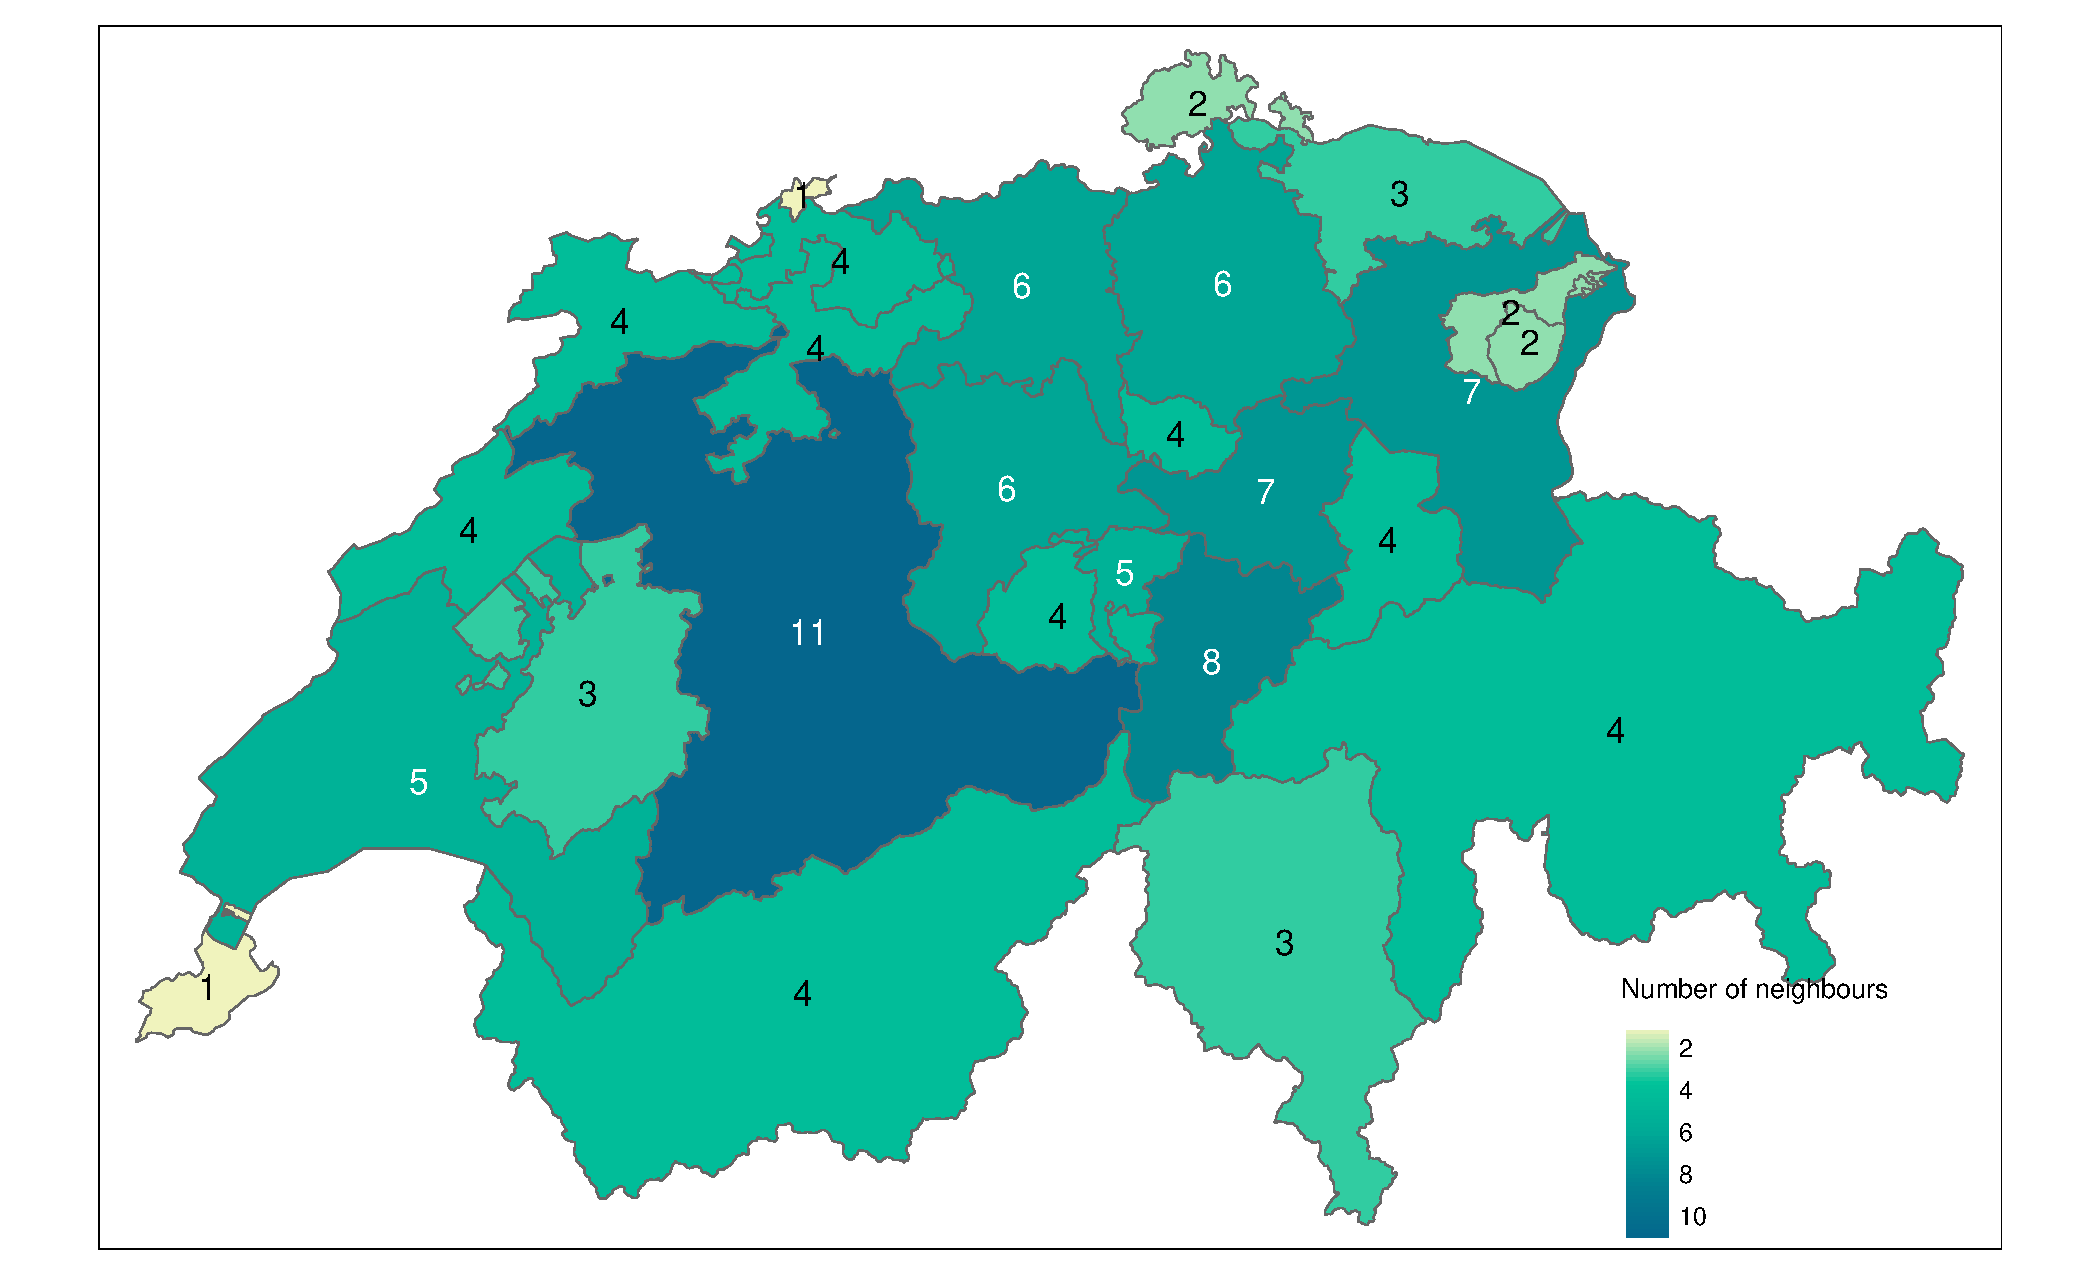
\includegraphics[page=1,width=\textwidth]{neighbours.pdf}
 \caption{The number of shared borders of cantons in Switzerland}
 \label{fig:neighbour}
\end{figure}
\subsubsection{Moran's I}\label{sec:moran}
Moran's I is a measure of spatial autocorrelation developed by Patrick Moran. Spatial autocorrelation is characterised by a correlation in a signal between close locations in space. Spatial autocorrelation is inherently more complex than one-dimensional autocorrelation due to the fact that spatial correlation is multidimensional (i.e. 2 or 3 spatial dimensions) and multi-directional. The formula for Moran's I is given by
\begin{equation}
    I = \frac{n}{W}\frac{\sum_{i=1}^n\sum_{j=1}^nw_{ij}\left(x_i-\overline{x}\right)\left(x_j-\overline{x}\right)}{\sum_{i=1}^n},
\end{equation}
with $n$ denoting the number of spatial units indexed by $i$ and $j$, $x$ the parameter of interest, $\pmb{w}$ a spatial neighbourhood matrix and $W$ the sum of all $w_{ij}$. \\
Using Moran's I, a test for spatial autocorrelation can be constructed with the following hypotheses:
\begin{align}
    H_0:\hbox{ No spatial autocorrelation} \hbox{ vs. }  H_1:\hbox{ Spatial autocorrelation}.
\end{align}
Under $H_0$ the expected value is given by
\begin{equation}
    \mathbb{E}\left[I\right]=\frac{-1}{n-1}.
\end{equation}
As $n$ approaches infinity, the expected value therefore approaches 0 \autocite[][]{moran1950notes}.
\subsubsection{Standardised Incidence Ratio}\label{sec:sir}
A basic measure of disease risk is the \textit{standardised incidence ratio}, which yields an estimate in each of the areas that form a partition of the study region. It is defined as the ratio of observed counts to expected counts
\begin{equation}\label{eq:sir}
    \hbox{SIR}_i = \frac{Y_i}{E_i}.
\end{equation}
$E_i$ represents the sum of the expected number of cases of a given area $i$ that behave according to the way the standard population behaves. It is calculated using indirect standardisation as
\begin{equation}
    E_i=\sum_{j=1}^mr_j^{(s)}n_j^{(i)},
\end{equation}
with $r_j^{(s)}$ the rate in stratum $j$ in the standard population and $n_j^{(i)}$ the population in stratum $j$ of area $i$. If the stratum information is unavailable, the expected counts can be calculated as follows
\begin{equation*}
    E_i = r^{(s)}n^{(i)},
\end{equation*}
where $r^{(s)}$ denotes the rate in the standard population and $n^{(i)}$ is the population of area $i$. If the standardised incidence rate is greater than 1, area $i$ has a higher risk than expected from the standard population, while for $\hbox{SIR}_i = 1$ the risk is the same and for $\hbox{SIR}_i < 1$ it is lower than expected. The ratio is also called the standardised mortality ratio when applied to mortality data \autocite[][]{moraga2019geospatial}.
\subsubsection{Spatial Small Area Disease Risk Estimation}\label{sec:spatial}
While SIRs may prove useful in some situations, in areas with low population sizes or rare diseases, expected counts may be low, making SIRs insufficiently reliable for reporting. It is therefore preferable to assess disease risk using models that allow information to be borrowed from neighbouring areas and incorporate information from covariates, thus smoothing or shrinking extreme values due to small sample sizes \autocite[][]{gelfand2010handbook}. \\
The observed counts $Y_i$ in area $i$ are typically modeled with a Poisson distribution with mean $E_i\theta_i$, where $E_i$ is the expected counts and $\theta_i$ denotes the relative risk in area $i$. To account for extra Poisson reliability, the logarithm of the relative risk is expressed as the total of the intercept and the random effects. $\theta_i$ quantifies whether area $i$ has a higher $\left(\theta_i >1\right)$ or lower $\left(\theta_i <1\right)$ risk than the average risk in the standard population. If the risk of an area $i$ is half the average risk, then $\theta_i = 0.5$. The general model for spatial data is formulated as follows:
\begin{align}
    Y_i&\sim\hbox{Po}\left(E_i\theta_i\right), \hspace{20pt} i=1,...,n,\\
    \log\left(\theta_i\right)&=\alpha+u_i+v_i.
\end{align}
The overall risk in the region of study is represented by $\alpha$, $u_i$ is a random effect specific to each area to model the spatial dependence between relative risks, and $v_i$ is an unstructured exchangeable component that models uncorrelated noise, $v_i\sim\mathcal{N}\left(0,\sigma_v^2\right)$. Covariates are often included to measure risk factors and other random effects to deal with different sources of variability. For example,
\begin{equation*}
    \log\left(\theta_i\right)=\pmb{d}_i\pmb{\beta}+u_i+v_i,
\end{equation*}
with $\pmb{d}_i = \left(1,d_{i1},...,d_{ip}\right)$ a vector of the intercept and $p$ covariates corresponding to the area $i$ and $\pmb{\beta}=\left(\beta_0,...,\beta_p\right)^T$ the vector of coefficients. An increase in $d_j\,\left(j = 1,...,p\right)$ by one unit, leads to an increase in the relative risk by a factor of $\exp\left(\beta_j\right)$, provided that all other covariates remain constant \autocite[][]{moraga2019geospatial}.
% In the Besag-York-Mollié (BYM) \autocite[][]{besag1991bayesian} model, this spatial random effect $u_i$ is assigned a conditional autoregressive (CAR) distribution that smooths the data according to a given neighbourhood structure that defines two areas as neighbours if they share a common boundary \autocite[][]{moraga2019geospatial}.
\subsubsection{Spatio-Temporal Small Area Disease Risk Estimation}\label{sec:spatiotemporal}
When disease counts are monitored over time, spatio-temporal models are useful as they take into account not only the spatial structure but also temporal correlations and spatio-temporal interactions \autocite[][]{martinez2008autoregressive}. Let $Y_{ij}$ be the counts observed in area $i$ and at time $j$, $\theta_{ij}$ be the relative risk, $E_{ij}$ be the expected number of cases in area $i$ and at time $j$, then
\begin{equation}
    Y_{ij}\sim\hbox{Po}\left(E_{ij}\theta_{ij}\right), \hspace{20pt} i=1,...,I,\,j=1,...,J.
\end{equation}
$\log\left(\theta_{ij}\right)$ is written as the sum of several components, including spatial and temporal structures, to consider that neighbouring areas and successive times may have similar risk. Spatio-temporal interactions can be included to account for the fact that temporal trends may differ from area to area but may be more alike in neighbouring areas. \\
Bernardinelli et al. \autocite[][]{bernardinelli1995bayesian}, for example, propose a spatio-temporal model with parametric time trends that expresses the logarithm of relative risks as
\begin{equation}
    \log\left(\theta_{ij}\right)=\alpha+u_i+v_i+ \left(\beta+\delta_i\right)\times t_j.
\end{equation}
The intercept is denoted by $\alpha$, $u_i+v_i$ is a random area effect, $\beta$ represents a global linear trend effect and $\delta_i$ is an interaction between space and time which is the difference between $\beta$ and the area-specific trend. For modeling $u_i$ and $\delta_i$, a CAR distribution is used and $v_i$ is i.i.d.. This specification allows each of the areas to have its individual time trend, where the spatial intercept is given by $\alpha+u_i+v_i$ and the slope by $\beta+\delta_i$. $\delta_i$ is referred to as the differential trend of the $i$-th area and represents the amount by which the time trend of area $i$ deviates from the overall time trend $\beta$. If $\delta_i\neq 0$, then area $i$ has a time trend with a slope that is either steeper or less steep than the overall time trend $\beta$. \\
For models that do not demand linearity of the time trend, non-parametric models such as the one proposed by Knorr-Held \autocite[][]{knorr2000bayesian} can be used. This specific model incorporates spatial effects, temporal random effects and an interaction between space and time as follows:
\begin{equation}
    \log\left(\theta_{ij}\right)=\alpha+u_i+v_i+\gamma_j+\phi_j+\delta_{ij}.
\end{equation}
The intercept is again denoted by $\alpha$, $u_i + v_i$ is a spatial random effect defined as before, i.e. $u_i$ follows a CAR distribution and $v_i$ is i.i.d.. $\gamma_j+\phi_j$ represents a temporal random effect and $\gamma_j$ follows either a first order random walk in time (RW1)
\begin{equation}
    \gamma_j|\gamma_{j-1}\sim\mathcal{N}\left(\gamma_{j-1},\sigma_\gamma^2\right),
\end{equation}
or second order random walk in time (RW2)
\begin{equation}
    \gamma_j|\gamma_{j-1},\gamma_{j-2}\sim\mathcal{N}\left(2\gamma_{j-1}-\gamma_{j-2},\sigma_\gamma^2\right).
\end{equation}
The unstructured temporal effect is given by $\phi_j\overset{i.i.d.}{\sim}\mathcal{N}\left(0, \sigma_\phi^2\right)$. The interaction between space and time, $\delta_{ij}$, can be specified in a number of ways by combining the structure of the random effects that interact. The interactions proposed by Knorr-Held are those between the effects $\left(u_i,\gamma_j\right)$, $\left(u_i,\phi_j\right)$, $\left(v_i,\gamma_j\right)$ and $\left(v_i,\phi_j\right)$ \autocite[][]{knorr2000bayesian}. \\
Using the last of these interactions leads to the assumption that there is no spatial or temporal structure on $\delta_{ij}$. Thus, the interaction term can be modeled as \\ $\delta_{ij}\sim\mathcal{N}\left(0,\sigma_\delta^2\right)$ \autocite[][]{moraga2019geospatial}.
\subsubsection{Issues With Areal Data}
The analysis of spatially aggregated data is subject to the "misaligned data problem" (MIDP), which arises when the data to be analysed is at a different scale from that at which it was collected \autocite[][]{banerjee2014hierarchical}. This may be solely due to the fact that the aim is to obtain the spatial distribution of a variable at a new spatial level of aggregation, e.g. if predictions are to be made at the county level with data that was originally collected at the postcode level. Another objective may be to try to find an association between variables available at different spatial scales, e.g. determining whether the risk of an unfavourable outcome provided at the country level correlates with exposure to an environmental pollutant measured at different stations, taking into account the population at risk and other demographic information available at the postcode level.\\
The Modifiable Area Unit Problem (MAUP) \autocite[][]{openshaw1984modifiable} describes a problem where the inference may differ when the same underlying data are grouped at a new spatial level of aggregation. It consists of two interrelated effects, the first of which is the scale/aggregation effect. It relates to the different conclusions obtained when the same data are grouped into larger and larger areas. The other effect is the grouping/zoning effect, which accounts for the variability in results due to alternative formations of the areas, resulting in differences in area shape given the same or similar scales. \\
Ecological studies are defined by their reliance on aggregated data \autocite[][]{robinson2009ecological} and the inherent potential for ecological fallacies. This phenomenon occurs when estimated associations obtained from the analysis of variables measured at the aggregate level lead to conclusions that differ from analyses based on the same variables measured at the individual level. This can be considered a special case of MAUP and the resulting so-called ecological bias is composed of two effects similar to the aggregation and zoning effects in MAUP. Namely, the aggregation bias caused by the aggregation of individuals and the specification bias due to the different distribution of confounding variables that results from the aggregation \autocite[][]{gotway2002combining, moraga2019geospatial}.
% \subsection{Geostatistical Data}
% Geostatistical data are measurements of one or more spatially continuous features collected at specific locations. They can be a disease risk measured by a survey in different villages, the level of a pollutant recorded at several monitoring stations, or the density of mosquitoes responsible for disease transmission measured by traps set at different locations \autocite[][]{waller2004applied}. Let $Z\left(s_1\right), ..., Z\left(s_n\right)$ be the observations of a spatial variable $Z$ at locations $s_1,...,s_n$. Geostatistical data are often assumed to be partial realisations of a random process
% \begin{equation}
%     \left\lbrace Z\left( s\right):s\in D\subset\mathbb{R}^2\right\rbrace,
% \end{equation}
% where $D$ denotes a fixed subset of $\mathbb{R}^2$ and the spatial index $\pmb{s}$ varies continuously over $D$. For practical reasons, it is only possible to observe $Z\left(\cdot\right)$ at a finite set of locations. The inference of the characteristics, e.g. mean and variability of the process, of the spatial process is based on this partial realisation. Using these characteristics, it is possible to predict the process at unobserved locations and construct a spatially continuous surface of the variable of interest.
% \subsubsection{Stochastic Partial Differential Equation Approach}
% With geostatistical data, an underlying spatially continuous variable can often be assumed and modelled using a Gaussian random field. A spatial model can be fitted using the stochastic partial differential equation (SPDE) approach and the variable of interest can be predicted at new locations. A GRF with a Matérn covariance matrix can be written as a solution to the following continuous domain SPDE \autocite[][]{whittle1963stochastic}:
% \begin{equation}
%     \left(\kappa^2-\Delta\right)^{\alpha/2}\left(\tau x\left(\pmb{s}\right)\right) = \mathcal{W}\left(\pmb{s}\right).
% \end{equation}
% The GRF is represented by $x\left(\pmb{s}\right)$, where smoothness is controlled by $\alpha$, while $\mathcal{W}\left(s\right)$ denotes a Gaussian spatial white noise process. $\kappa>0$ is a scale parameter and $\Delta$ denotes the Laplacian given by $\sum_{i=1}^d\frac{\partial^2}{\partial x_i^2}$, where $d$ is the dimension of the spatial domain D. \\
% The smoothness parameter $\nu$ of the Matérn covariance function is linked to the SPDE by
% \begin{equation*}
%     \nu=\alpha-\frac{d}{2}
% \end{equation*}
% while the marginal variance $\sigma^2$ is related to the SPDE by
% \begin{equation*}
%     \sigma^2=\frac{\Gamma\left(\nu\right)}{\Gamma\left(\alpha\right)\left(4\pi\right)^{d/2}\kappa^{2\nu}\tau^2}.
% \end{equation*}
% For $d=2$ and $\nu=0.5$ this corresponds to the exponential function. \\
% The SPDE can be solved approximately using the \textit{finite element} method, which partitions the spatial domain $D$ into a set of non-intersecting triangles, resulting in a triangulated mesh with $n$ vertices and $n$ basis functions $\psi_k\left(\cdot\right)$. These functions are piecewise linear functions on each triangle, equal to 1 at vertex $k$ and 0 otherwise. The continuously indexed Gaussian field $x$ is thus represented as a discretely indexed Gaussian Markov random field by the finite basis functions defined on the triangulated mesh
% \begin{equation}
%     x\left(\pmb{s}\right)=\sum_{k=1}^n\psi_k\left(\pmb{s}\right)x_k,
% \end{equation}
% with $n$ the number of vertices of the triangulate, $\psi_k\left(\cdot\right)$ the piecewise linear basis functions and $\left\lbrace x_k\right\rbrace$ zero-mean Gaussian distributed weights. \\
% The joint distribution of the weight vector follows a Gaussian distribution, $\pmb{x}=\left(x_1,... ,x_n\right)\sim\mathcal{N}\left(0, \pmb{Q}^{-1}\left(\tau, \kappa\right)\right)$, which approximates the solution $x\left(\pmb{s}\right)$ of the SPDE in the mesh nodes, and the basis functions transform $x\left(\pmb{s}\right)$ from the mesh nodes to the other spatial locations of interest \autocite[][]{lindgren2011explicit}.
% !TEX root = ../my-thesis.tex
%
\chapter{Dataset Collection}
Having established the methodology that is used in this work, it is now time to move on to the analytical part of this work, starting with the collection of data. The construction of the dataset used to analyse a research question is an essential task and frequently involves the merging of multiple data sources to create one final dataset. In particular, the analysis of data on Covid-19 requires the pooling of numerous data sources due to the sheer volume of data available on this disease. The following chapter a brief overview of the data sources used, their pre-processing and how they are combined is given. All the data that is used in this work is openly available, either through government sources, GitHub or the use of R packages.
\label{sec:datacollection}
\clearpage
\section{Covid-19 Data}
\subsection{Covid-19 Data for Norway}
The Covid-19 data for Norway comes from a dataset made available to the public via a repository on the website \href{https://www.github.com}{GitHub.com}, created by the user thohan88. The repository contains a daily updated dataset that is the result of combining several data sources, which include the Norwegian Institute of Public Health and the Norwegian Directorate of Health. According to the author of the repository, the project is "an open-source effort to make data about the Covid-19 situation in Norway available to the public in a timely and coherent manner" \autocite[][]{thohan88}. \\
A few sample data points from this dataset are displayed in Table~\ref{datasetNorge}.\\
\begin{table}[H] 
\caption{An excerpt from the Covid-19 data for Norway. Does not contain all variables. The number of infections are the cumulative number of infections. \label{datasetNorge}}
\begin{tabular}{l l r r r}
\toprule
\textbf{Id}	& \textbf{Municipality}	& \textbf{Population}	& \textbf{Inf. 2020-03-26}	& \textbf{Inf. 2020-03-27}\\
\midrule
1103 & Stavanger & 143574 & 87 & 88 \\
1507 & Ålesund & 66258 & 20 & 20 \\
4601 & Bergen & 283929 & 231 & 248 \\
5001 & Trondheim & 205163 & 113 & 136 \\
\bottomrule
\end{tabular}
\end{table}
\subsection{Covid-19 Data for Germany}
In Germany, the Robert Koch Institute publishes daily situation reports in which the number of new cases is published at NUTS 3 level. These reports are available as PDF files via the Institute's website. They can be downloaded and grouped via the R package \texttt{covid19germany}\autocite[][]{covid19germany}, as is done for this work.\\
A few sample data points from this dataset are displayed in Table~\ref{datasetGermany}.
\begin{table}[H] 
\caption{An excerpt from the Covid-19 data for Germany. Does not contain all variables.\label{datasetGermany}}
\begin{tabular}{l l r r r}
\toprule
\textbf{Municipality}	& \textbf{Date}	& \textbf{Cumulative number of infections} & \textbf{Population}\\
\midrule
SK München & 2020-01-29 & 1 & 1471508\\
SK München & 2020-02-03 & 2 & 1471508\\
SK München & 2020-02-11 & 3 & 1471508\\
LK Rosenheim & 2020-02-29 & 1 & 260983\\
LK Rosenheim & 2020-03-08 & 2 & 260983 \\
LK Rosenheim & 2020-03-10 & 6 & 260983 \\
\bottomrule
\end{tabular}
\end{table}
\clearpage
\section{Vaccination Data}
At the end of 2020, the first countries began vaccinating against Covid-19. Vaccination leads to a milder course of the disease, but it is not yet known whether vaccinated people can continue to transmit Covid-19, as of early May 2021. By including the proportion of people vaccinated, an indication as to how much vaccination helps prevent the spread of Covid-19 can potentially be given. These data are available for Norway at the municipality level via the statistics database of the Norwegian Institute of Public Health, FHI \autocite[][]{fhi}. For Germany, these data are only available at the state level and are therefore not used.
\clearpage
\section{Demographic Data}
As demographics tend to differ between different geographic units, the decision is made to include demographic variables in the analysis of the research question to see if the risk for infection may be higher when a certain characteristic is present in the population.
\subsection{Demographic Data for Norway}
The demographic data that is collected for Norway comes from Statistisk Sentralbyrå and is made available to the public through their online database, StatBank \autocite[][]{ssb}. \\
The first characteristic collected is the age of the population in a given municipality. For each age, starting at 0 and ending at 105, the number of people of that age is known. \\
Next, unemployment data are collected for a given municipality. For each municipality, the percentage of all people out of work is known, as well as the percentage of all immigrants out of work. \\
Other data that is collected includes data related to the number of workers in a particular industry, as well as immigration data. Since there is discussion about whether workers from certain industries, in this case the construction industry, contribute to the spread of Covid-19, the decision is made to collect this type of data. For each community, the number of workers across all industries is known, as well as the number of workers in the construction industry. Workers, in this case, are individuals employed in a given municipality who are between the ages of 20 and 66. It is known how many people work full-time and how many people work part-time. \\
Finally, for immigration data, it is known how many immigrants live in a given municipality and how many Norwegians are born to immigrant parents. These figures are known in terms of the percentage of the population in 2020.
\subsection{Demographic Data for Germany}
The demographic data that is collected for Germany comes from the federal and state statistical offices and is made available to the public through their online database, Regionaldatenbank Deutschland \autocite[][]{rdb}. \\
The first characteristic that is collected is unemployment data at the NUTS 3 level. For each municipality, the number of unemployed people as well as the number of unemployed foreigners is collected. \\
Next, data related to the European elections in 2019 are collected. In each municipality, it is known how many people voted in total, how many people voted for the six largest parties, and how many votes the remaining parties received combined. \\
Data is collected in relation to people seeking protection, welfare recipients and in relation to asylum seeker benefits. It is known how many people seek protection in Germany, how many receive social welfare and how many receive asylum seeker benefits. Finally, trade tax, income tax, and payroll tax data are collected for each municipality. 
\clearpage
\section{Shapefiles}
In addition to numeric variables, the dataset contains a geographic variable containing the geographic boundaries of a given municipality or city/district.
\subsection{Shapefiles for Norway}
The data for the Norwegian shapefiles comes from Geonorge \autocite[][]{geonorge} and is downloaded from a GitHub repository, as the data there is in a cleaner state \autocite[][]{shapeGithub}. In addition to the geographic shape, the dataset includes a variable that contains the ID of each municipality.
\subsection{Shapefiles for Germany}
The data for the German shapefiles comes from Esri Germany \autocite[][]{esri}.
\clearpage
\section{OpenStreetMap Data}
OpenStreetMap (OSM) is a free project that collects, structures and stores freely usable geodata in a database for use by anyone (Open Data). This data is available under a free licence, the Open Database Licence. The core of the project is therefore an openly accessible database of all contributed geoinformation \autocite[][]{OpenStreetMap}. \\
In R, the OpenStreetMap API can be queried using the R package \texttt{osmdata} \autocite[][]{osmdata}. To download all locations of a given type in a given region, a shape or bounding box must be specified along with a key and optionally a value. These key-value pairs are used to specify the type of location, for example, the "amenity" key is used for all facilities used by visitors and residents. If the "biergarten" value is used together with the "amenity" key, the locations of all beer gardens in a given geographic region is downloaded. \\
OpenStreetMap's users have the option to map a location as either \texttt{POINT}, \texttt{POLYGON}, \texttt{MULTIPOLYGON}, \texttt{LINESTRING}, or \texttt{MULTILINESTRING}. Conventionally, the first three are used. Therefore, only sites mapped as one of these are used for this work. If a location is mapped as either \texttt{POLYGON} or \texttt{MULTIPOLYGON}, the centroid of the location is calculated. \\
A complete list of all key-value pairs used for this work can be found in Section~\ref{sec:kv} in the Appendix. 
\clearpage
\section{Government Response and Mobility Data}
Our World in Data (OWID) is an online publication that provides information on the historical development of human living conditions. It looks at demographic, developmental economic, geographical and cultural aspects, among others. Our World in Data often takes a historical perspective and provides information on the historical development of humanity's living conditions. \\
OWID is structured according to problem areas. Each article discusses a global problem - from health problems, to hunger, poverty, war, education, to environmental issues. Depending on the completeness of the entry, these present the historical development of an aspect, the causes and consequences of this development, and the quality of the underlying data. All topics are also presented graphically. \\
On their website, they provide statistics on governments' policy responses to the coronavirus pandemic. These statistics come from the Oxford Coronavirus Government Response Tracker (OxCGRT), which contains data from public sources collected by a team of over a hundred Oxford University students and staff from around the world. The tracker contains 17 indicators ranging from containment and closure policies, e.g. school closures, to economic policies such as income support and health system policies, e.g. testing regimes. 9 of these indicators are used to calculate a Government Stringency Index, which scales from 0 to 100, with 100 denoting the most stringent government policies \autocite[][]{hale2020variation, ritchie2020coronavirus}. \\
Besides government responses, another type of data available through OWID, are the mobility reports by Google. The mobility reports are designed to provide information on what has changed as a result of the regulations to address the Corona crisis. The reports present movement trends broken down by geographic regions and place categories - for example, retail and recreation, grocery shops, parks, public transport stations and stops, places of work and places of residence. To do this, Google measures the number of visitors to these locations each day and compares them to a pre-pandemic base day. A base day represents a normal value for that day of the week, given as a median value over the five-week period from 3 January 2020 to 6 February 2020 \autocite[][]{googlemobility, ritchie2020coronavirus}
\clearpage
\section{Covid-19 Variants Data}
The last data source is the open source project CoVariants. The project provides an overview of SARS-CoV-2 variants and mutations of interest. It tracks for different countries the proportion of the total number of sequences (not cases) over time that fall into defined variant groups, such as the B.1.1.7. variant, better known as the UK variant of Covid-19. In addition to the prevalence of the different variants, the project also provides data on the common mutations between the different strains, but this is not of interest in this work \autocite[][]{hodcroft2021covariants}.
\clearpage
\section{Data Wrangling}
The final step before analysing the research question at hand is to combine all of these data sources into one dataset. This section shows how this is achieved.
\subsection{Data Wrangling for Norway}
The initial step in creating the final dataset is to convert the data from a wide format, as seen in Table~\ref{datasetNorge}, to a long format. This is done using the function \texttt{melt()} from the R package \texttt{reshape2} \autocite[][]{reshape2}. The long version of the dataset is shown in Table~\ref{norwayLong}.
\begin{table}[H] 
\caption{An excerpt from the long version of the Norwegian Covid-19 data. Does not contain all variables.\label{norwayLong}}
\begin{tabular}{l l r r r}
\toprule
\textbf{Id}	& \textbf{Municipality}	& \textbf{Population} & \textbf{Date} & \textbf{Infections}\\
\midrule
1507 & Ålesund & 66258 & 2020-03-26 & 20\\
5001 & Trondheim  & 205163  & 2020-03-26 & 113\\
1507 & Ålesund & 66258 & 2020-03-27 & 20\\
5001 & Trondheim  & 205163  & 2020-03-27 & 136\\
\bottomrule
\end{tabular}
\end{table}
Next, the demographic data for Norway is loaded and processed. Since the age data contains the number of people of a certain age, the median age is calculated for each region based on how many people of each age group live in each region. \\
The other demographic variables are left unchanged. To combine the demographic data with the Covid-19 data, the municipality IDs are extracted using the \texttt{str\_extract()} function from the \texttt{stringr} \autocite[][]{stringr} R package using the regular expression \texttt{[0-9]\{4\}}. Next, all demographic datasets and the Covid-19 dataset are merged using the \texttt{merge()} function. \\
Using the \texttt{st\_intersects()} function from the \texttt{sf} \autocite[][]{sf} R package, the number of points of interest downloaded via OpenStreetMap is calculated for each municipality. Since the shapefiles contain the ID for each community, these data are merged with the data containing the demographic and Covid-19 data. \\
For each numeric variable, e.g. the number of schools or the number of employees, this number is scaled. \\
If there are missing values in the covariates, these values are imputed using the median of the respective variable. 
\clearpage
Next, the vaccination data for Norway is loaded. As the daily number of vaccinated persons for each municipality is included in the data, these numbers only need to be cumulated before being merged with the rest of the data based on municipality name and date. \\
Finally, seven new variables are created:
\begin{itemize}
    \item[1.] Expected count, which is the expected number of cases in each municipality.
    \item[2.] SIR, which is the standardized incidence ratio in each municipality.
    \item[3.] An area ID, which is a unique ID given to each municipality.
    \item[4.] Higher education, which counts the number of universities and colleges in a given area.
    \item[5.] Sex, which gives the proportion of females living in a given area.
    \item[6.] Population density, i.e. the number of people per square kilometre in a given area.
    \item[7.] Urban density, i.e. the number of residential buildings per square kilometre in a given area.
\end{itemize}
The final dataset contains the variables shown in Table~\ref{datasetNorway}. $\newline\newline\newline\newline\newline\newline\newline\newline\newline\newline\newline\newline\newline\newline\newline\newline\newline\newline\newline$
\begin{table}[H] 
\caption{The variables contained in the final dataset.\label{datasetNorway}}
\begin{tabular}{l l l}
\toprule
\textbf{Variable Name}	& \textbf{Explanation}	& \textbf{Scale}\\
\midrule
Id & The municipality ID & None \\
Municipality & The municipality name & None \\
Population & Population in a municipality & None \\
Date & The date of the data used & None \\
Infections & The number of infected people & None \\
Median age & The median age & scaled \\
\multirow{2}{*}{Total unemployment} & The proportion of &\multirow{2}{*}{scaled}\\
& unemployed people \\
\multirow{2}{*}{Unemployed immigrants} & The proportion of & \multirow{2}{*}{scaled}\\
 & unemployed immigrants  \\
\multirow{2}{*}{Full-time workers} & The number of & \multirow{2}{*}{scaled} \\
& full-time workers \\
\multirow{2}{*}{Part-time workers} & The number of & \multirow{2}{*}{scaled} \\
& part-time workers \\
\multirow{2}{*}{Full-time construction} & The number of full-time & \multirow{2}{*}{scaled} \\
& construction workers \\
\multirow{2}{*}{Part-time construction} & The number of part-time & \multirow{2}{*}{scaled} \\
& construction workers \\
Total immigrants & The proportion of immigrants  & scaled \\
Marketplace & The number of marketplaces & scaled \\
Entertainment & The number of entertainment venues & scaled \\
Sport & The number of sports amenities & scaled \\
Clinic & The number of clinics & scaled \\
Hairdresser & The number of hairdresser & scaled \\
Shops & The number of shops & scaled \\
Place of worship & The number of places of worship & scaled \\
Retail & The number of retail stores & scaled \\
Nursing home & The number of nursing homes & scaled \\
Restaurant & The number of restaurants & scaled \\
Aerodrome & The number of aerodromes & scaled \\
Office & The number of offices & scaled \\
\multirow{2}{*}{Platform} & The number of public & \multirow{2}{*}{scaled} \\
& transport platforms \\
Kindergarten & The number of kindergartens & scaled \\
Schools & The number of schools & scaled \\
Bakeries & The number of bakeries & scaled \\
Residential & The number of residential buildings & None \\
\multirow{2}{*}{Higher education} & The number of colleges & \multirow{2}{*}{scaled} \\
& and universities \\
Expected count & The expected number of infections & None \\
SIR & The standardized incidence ratio & None \\
Area Id & A unique ID & None \\
Area & The area in km$^2$ & None \\
Population density & People per km$^2$ & scaled\\
\multirow{1}{*}{Urban density} &  Residential buildings per km$^2$ & scaled \\
Sex & The proportion of females & scaled \\
Vaccinations & The proportion of vaccinated & scaled \\
\bottomrule
\end{tabular}
\end{table}
\subsection{Data Wrangling for Germany}
The data processing procedure for Germany is identical to that for Norway. First, all demographic variables are loaded and left unchanged before being merged with the Covid-19 data prior to calculating the spatial intersections between the points of interest and the NUTS-3 areas. After merging all the data, the scaled numbers are calculated for the numeric variables. For the variables containing the number of people who voted for a particular political party, the relative percentage of votes the party received is calculated. Again, missing values are imputed using the median.
Finally, the same seven new variables are created. 
The final dataset contains the variables shown in Table~\ref{finalGermany}.
$\newline\newline\newline\newline\newline\newline\newline\newline\newline\newline\newline\newline\newline\newline\newline\newline\newline\newline\newline\newline\newline\newline\newline\newline\newline\newline\newline\newline$
\begin{table}[H] 
\caption{The variables contained in the final dataset.\label{finalGermany}}
\begin{tabular}{l l l}
\toprule
\textbf{Variable Name}	& \textbf{Explanation}	& \textbf{Scale}\\
\midrule
Id & The municipality ID & None\\
Municipality & The municipality name & None \\
Population & Population in a municipality & None \\
Date & The date of the data used & None\\
Infections & The number of infected people & None \\
Logarithmic trade tax & The trade tax in Euros & scaled \\
Logarithmic income tax & The income tax in Euros & scaled \\
Logarithmic total income & The income and payroll tax in Euros & scaled \\
\multirow{2}{*}{Asyl benefits} & The number of people & \multirow{2}{*}{scaled} \\
& receiving asylum seeker benefits \\
Welfare recipients & The number of welfare recipients & scaled \\
Unemployed people & The number of unemployed people & scaled \\
Unemployed foreigners & The number of unemployed foreigners & scaled \\
Protection seekers & The number of protection seekers & scaled \\
Die Union & Percentage of vote for Union & scaled\\
SPD & Percentage of vote for SPD & scaled\\
Greens & Percentage of vote for the Greens & scaled\\
FDP & Percentage of vote for FDP & scaled\\
The left & Percentage of vote for the left & scaled\\
AfD & Percentage of vote for AfD & scaled \\
Marketplace & The number of marketplaces & scaled \\
Entertainment & The number of entertainment venues & scaled \\
Sport & The number of sports amenities & scaled \\
Clinic & The number of clinics & scaled \\
Hairdresser & The number of hairdresser & scaled \\
Shops & The number of shops & scaled \\
Place of worship & The number of places of worship & scaled \\
Retail & The number of retail stores & scaled \\
Nursing home & The number of nursing homes & scaled \\
Restaurant & The number of restaurants & scaled \\
Aerodrome & The number of aerodromes & scaled \\
Office & The number of offices & scaled \\
\multirow{2}{*}{Platform} & The number of public & \multirow{2}{*}{scaled} \\
& transport platforms \\
Kindergarten & The number of kindergartens & scaled \\
Schools & The number of schools & scaled \\
Bakeries & The number of bakeries & scaled \\
Residential & The number of residential buildings & None \\
\multirow{2}{*}{Higher education} & The number of colleges & \multirow{2}{*}{scaled} \\
& and universities \\
Expected count & The expected number of infections & None \\
SIR & The standardized incidence ratio & None \\
Area Id & A unique ID & None \\
Area & The area in km$^2$ & None \\
Population density & People per km$^2$ & scaled  \\
\multirow{1}{*}{Urban density} & Residential buildings per km$^2$  & scaled\\
Sex & The proportion of females & scaled \\
\bottomrule
\end{tabular}
\end{table}
\subsection{Data Wrangling for the Temporal Models}
Obtaining data for the temporal models is simple. OWID provides a dataset that includes case numbers for over 200 countries, along with vaccination numbers for that country, among other variables. Next, all data related to government response and mobility data are loaded. As these data are not available over the same time period for each country, some assumptions are made to minimize missing data. These assumptions are
\begin{itemize}
    \item If vaccination data before the administration of the first vaccine dose in a country are missing, no people were vaccinated at these points in time.
    \item If vaccination data are missing for time points after the last available data, the vaccination rate has remained the same.
    \item If government policy data are missing before the first recorded government response to a particular policy, then the policy is "No response".
    \item If government policy data are missing after the last tracked government response to a particular policy, then the policy has remained the same since that time.
    \item If mobility data is missing between points in time, then a constant decline / slope is assumed for this data.
\end{itemize}
After imputing all missing values, the next step is to merge these data. This can be done simply by using the unique combinations between the date and the country variable. In the last step, instead of using the infection figures provided by OWID, which mostly come from Johns Hopkins University, the infection figures that are also used for the spatial models are used, as these come from official government sources. \\
The final dataset contains the variables shown in Table~\ref{datasetTimeseries}.$\newline\newline\newline\newline\newline\newline\newline\newline\newline$
\begin{table}[H] 
\caption{The variables contained in the final dataset.\label{datasetTimeseries}}
\begin{tabular}{l l l}
\toprule
\textbf{Variable Name}	& \textbf{Explanation}	& \textbf{Scale}\\
\midrule
Country Code & The iso2 code of a country & None \\
Country & The name of a country & None \\
Population & Population in a municipality & None \\
Date & The date of the data used & None \\
Infections & The number of infected people & None \\
Mobility retail \& recreation & The change in mobility in retail \& recreation & scaled \\
Mobility grocery \&& The change in mobility in & \multirow{2}{*}{scaled} \\
pharmacies & groceries \& pharmacies \\
Mobility residential & The change in mobility in residential areas & scaled \\
Mobility transport stations  & The change in mobility at public transport areas & scaled \\
Mobility parks  & The change in mobility in parks & scaled \\
Mobility workplaces  & The change in mobility in workplaces & scaled \\
Testing policy & Policies implemented related to testing & factor \\
Contact tracing & Policies implemented related to contact tracing & factor \\
Vaccination policy & Policies implemented related to vaccination & factor \\
Facial coverings policy & Policies implemented related to facial coverings & factor \\
Income support & Policies implemented related to income support & factor \\
Restrictions on  & Policies implemented related to &  \multirow{2}{*}{factor} \\
internal movement & the restriction on internal movement \\
International travel & Policies implemented related to& \multirow{2}{*}{factor} \\
controls & international travel controls \\
Public information & Public information campaigns & \multirow{2}{*}{factor} \\
campaigns & on Covid-19 \\
Cancellation of & Policies implemented related to & \multirow{2}{*}{factor} \\
public events & the cancellation of public events \\
\multirow{2}{*}{Restriction of gatherings} & Policies implemented related to & \multirow{2}{*}{factor} \\
& the restriction of gatherings \\
\multirow{2}{*}{Closing of public transport} & Policies implemented related to & \multirow{2}{*}{factor} \\
& the closing of public transport \\
\multirow{2}{*}{Closing of schools} & Policies implemented related to& \multirow{2}{*}{factor} \\
& the closing of schools \\
\multirow{2}{*}{Closing of workplaces} & Policies implemented related to& \multirow{2}{*}{factor} \\
& the closing of workplaces \\
\multirow{2}{*}{Stay home requirements} & Policies implemented related to& \multirow{2}{*}{factor} \\
& stay home requirements \\
Stringency index & The government stringency index  & scaled \\
People vaccinated &  The proportion of people who have received   & scaled \\
per hundred  & at least 1 dose of a vaccine\\
People fully vaccinated & \multirow{2}{*}{The proportion of fully vaccinated people} &  \multirow{2}{*}{scaled} \\
per hundred \\
\multirow{2}{*}{Variant 20E} & The proportion of the total number of& \multirow{2}{*}{scaled} \\
& sequences of the 20E variant \\
\multirow{2}{*}{Variant 20L} & The proportion of the total number of& \multirow{2}{*}{scaled} \\
& sequences of the 20L variant \\
\multirow{2}{*}{Other variants} & The proportion of the total number of& \multirow{2}{*}{scaled} \\
& sequences that are not tracked \\
Season & The season of the date & factor \\
Expected count & The expected number of infections & None \\
\bottomrule
\end{tabular}
\end{table}
% !TEX root = ../my-thesis.tex
%
\chapter{Data Analysis}
\label{sec:analysis}
In this chapter the models calculated for each country are reviewed. First, a look at the standardised incidence rate for each country is taken, before spatial models, spatio-temporal models and finally predictive models are discussed.
\section{Standardised Incidence Ratio}
This section takes a brief look at the standardised incidence ratio for the countries of interest.
\subsection{Standardised Incidence Ratio for Germany}
When looking at the standardised incidence ratio for Germany, it is noticeable that the actual number of infections in the eastern parts of Germany, especially in Saxony, is considerably higher than the expected number of infections. Furthermore, parts of Bavaria have an increased standardised incidence ratio compared to the rest of Germany, excluding Saxony. This could be due to the fact that the regions share a border with the Czech Republic, a country that is substantially more affected by Covid-19 than Germany. The northern parts of Germany show the lowest SIR which is possibly due to the fact that this region is sparsely populated. For more information, see Figure~\ref{sirgermany}.
% \begin{figure}[H]
%   \centering
%   \includesvg[width = 1.2\textwidth]{sir_germany.svg}
%   \caption{The standardised incidence ratio for Germany based on the data of the 24th of March 2021}
%   \label{sirgermany}
% \end{figure}
\begin{figure}[H]
  \centering
  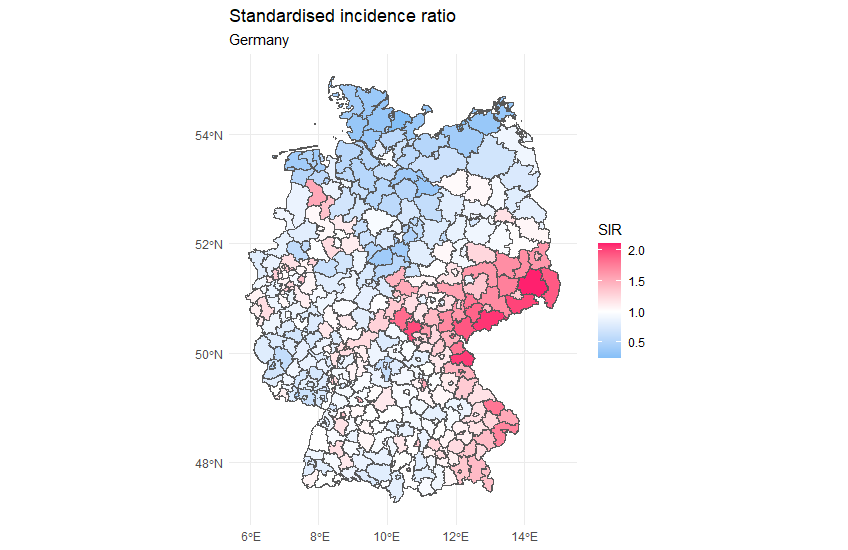
\includegraphics[width = 1.2\textwidth]{sir_germany.png}
  \caption{The standardised incidence ratio for Germany based on the data of the 24th of March 2021}
  \label{sirgermany}
\end{figure}
\subsection{Standardised Incidence Ratio for Norway}
Looking at the standardised incidence rate for Norway, a standardised incidence rate of less than 1 can be seen for most municipalities north of Trondheim. In the southern parts of Norway there are several municipalities with a rate above 1, for example the standardised incidence rate around the capital Oslo is around 2. However, the two small municipalities, Hyllestad and Ulvik, have the highest standardised incidence rate in Norway. In Hyllestad, 95 of 1328 people have been infected with Covid-19 so far, while in Ulvik, 134 of 1080 people have been infected so far. \\
The SIR in Hyllestad is around 4.5, following an outbreak in a shipyard in autumn 2020 \cite{newspaper1}, while Ulvik has a ratio of around 8, following an outbreak of the UK variant of Covid-19. According to the head of the municipality, Hans Petter Thorbjørnsen, the infections are thought to have spread through children \cite{newspaper2}. See Figure~\ref{sirnorway} for more information.
% \begin{figure}[H]
%   \centering
%   \includesvg[width = 1.2\textwidth]{sir_norway.svg}
%   \caption{The standardised incidence ratio for Norway based on the data of the 24th of March 2021}
%   \label{sirnorway}
% \end{figure}
\begin{figure}[H]
  \centering
  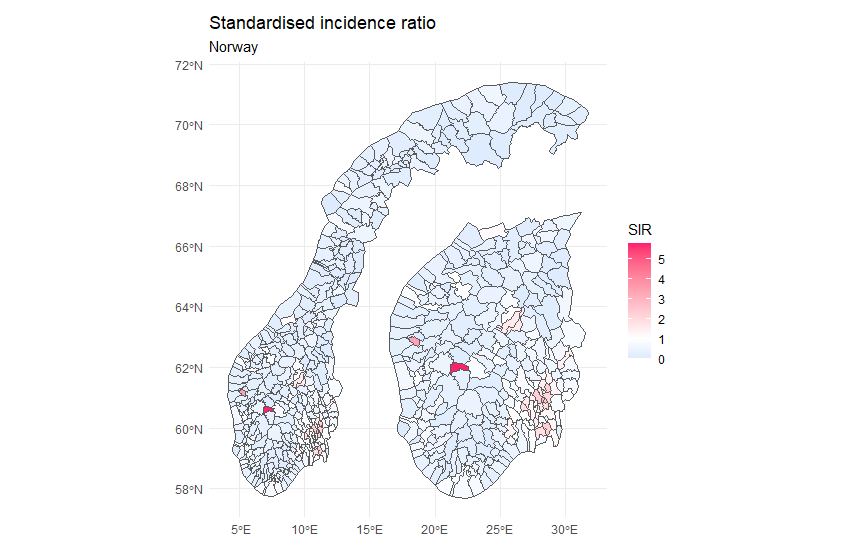
\includegraphics[width = 1.2\textwidth]{sir_norway.png}
  \caption{The standardised incidence ratio for Norway based on the data of the 24th of March 2021}
  \label{sirnorway}
\end{figure}
Because the high numbers from two small municipalities complicate the interpretation of Figure~\ref{sirnorway}, Figure~\ref{sirnorwaylog} shows the SIR on a log10 scale. It is now clearer that the standardized incidence ratio is below 1 in most parts of Norway, but that there is a higher risk in the region around Oslo.
% \begin{figure}[H]
%   \centering
%   \includesvg[width = 1.2\textwidth]{sir_norway_log.svg}
%   \caption{The log10 standardised incidence ratio for Norway based on the data of the 24th of March 2021}
%   \label{sirnorway}
% \end{figure}
\begin{figure}[H]
  \centering
  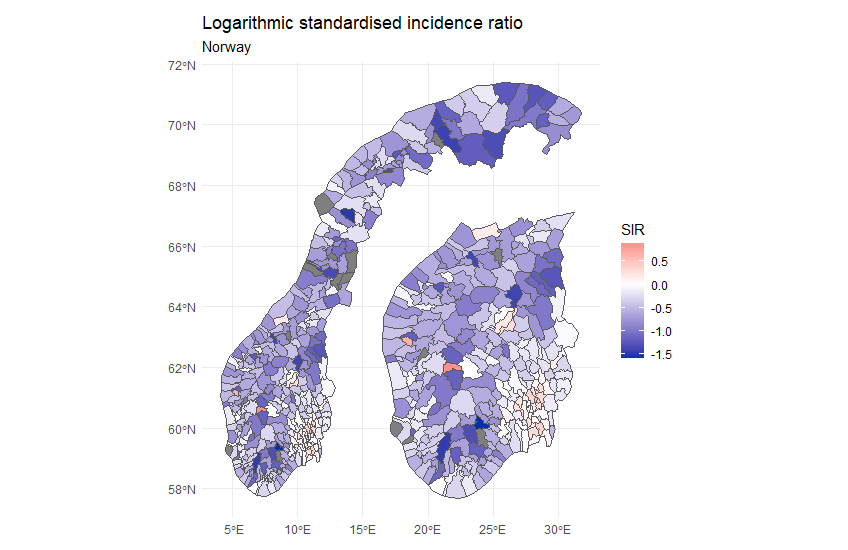
\includegraphics[width = 1.2\textwidth]{sir_norway_log.png}
  \caption{The log10 standardised incidence ratio for Norway based on the data of the 24th of March 2021}
  \label{sirnorwaylog}
\end{figure}
\clearpage
\section{Spatial Models}
After looking at the standardised incidence rates for the countries of interest, the next step is to take a closer look at the current figures for the respective countries. Spatial models are used to try to extract the factors that cause some populations to be at higher risk than other populations. Four different types of models are used for each country:
\begin{itemize}
    \item[1.] The Besarg-Yollie-Mollie Model
    \item[2.] Besags Proper Spatial Model
    \item[3.] The Leroux-Model
    \item[4.] A model without a spatial component
\end{itemize}
All of these models were computed using the INLA \cite{rinla} R package. \\
To specify each type of model, the code shown in Listing~\ref{codeModels} can be used. \\
Four measures are used to compare the models, the DIC, the WAIC, the CPO and the mean absolute error (MAE).\\
For all countries, the models were computed with
\begin{itemize}
    \item[1.] only the demographic variables as covariates
    \item[2.] only the infrastructural variables as covariates
    \item[3.] both, demographic and infrastructural variables, as covariates
    \begin{itemize}
        \item[3.1] Without variable selection
        \item[3.2] With variable selection
    \end{itemize}
\end{itemize}
In addition to specifying what type of spatial model to use, if any, there is also the option of specifying a prior. In this case, a penalised complexity prior is used for the precision $\tau$. For $\tau$, the penalised complexity prior is defined by the parameter $\sigma_0$. The equation~\ref{eq:pcprior} therefore looks like this,
\begin{equation}\label{pcprec}
    \mathbb{P}\left(\sigma > \sigma_0\right)=\alpha.
\end{equation}
The actual expression of the prior is given by
\begin{equation}
    \pi\left(\tau\right)=\frac{\lambda}{2}\tau^{-3/2}\exp\left(-\lambda\tau^{-1/2}\right),\hspace{10pt}\tau>0.
\end{equation}
Here, $\lambda=\frac{-\log\left(\alpha\right)}{U}$ \cite{martins2014penalising}.
For the parameters $\sigma_0$ and $\alpha$, the values 1 and 0.01 were chosen. \\
The models were compared using the mean absolute error. For this, 20\% of the observations were removed from the training and used for testing instead. The predicted number of infections for these municipalities was then compared to the actual numbers.
\\
Finally, due to the amount of covariates, forwards and backwards stepwise variable selection was performed with the intention of obtaining a model that fits the data well and at the same time is relatively easy to interpret. This can be done with the R package \texttt{INLAutils} \cite{inlautils}, as shown in Listing~\ref{codeSelection}. Backwards as well forwards variable selection was performed.\\
A list of all calculated models along with their performance measures is provided in the appendix.
\subsection{Model Selection}
Before the models are computed, however, the distribution that fits the number of cases must first be found. For this, the function \texttt{descdist()} from the \texttt{fitdistrplus} R package is used. The Cullen and Frey graph can be used to give an initial idea of which distributions fit the data, in this case the number of infections, reasonably well depending on the kurtosis and the square of the skewness. \\
The plots for Germany and Norway can be seen in Figure~\ref{cf_germany} and Figure~\ref{cf_norge}.
% \begin{figure}[H]
%     \centering
%     \includesvg[width = 0.8\textwidth]{cf_germany.svg}
%     \caption{The Cullen and Frey graph for Germany}
%     \label{cf_germany}
% \end{figure}
\begin{figure}[H]
    \centering
    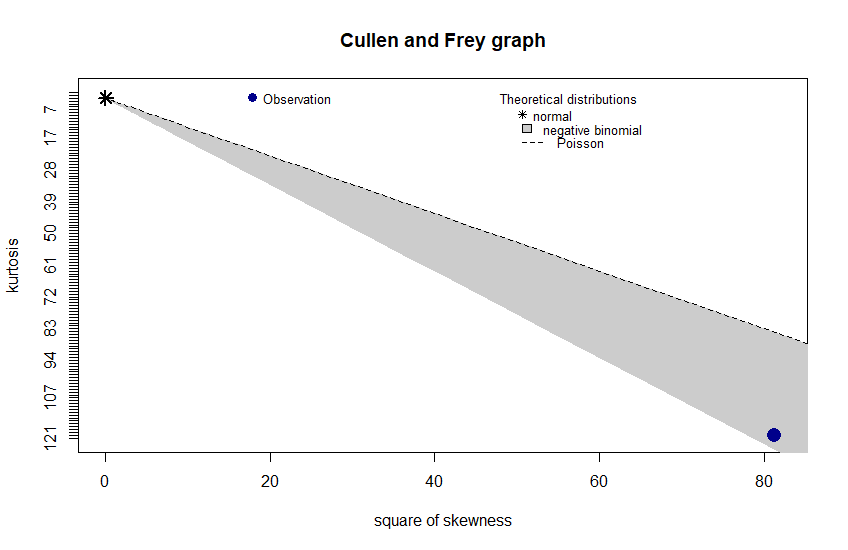
\includegraphics[width = 0.8\textwidth]{cf_germany.png}
    \caption{The Cullen and Frey graph for Germany}
    \label{cf_germany}
\end{figure}
% \begin{figure}[H]
%     \centering
%     \includesvg[width = 0.8\textwidth]{cf_norge.svg}
%     \caption{The Cullen and Frey graph for Norway}
%     \label{cf_norge}
% \end{figure}
\begin{figure}[H]
    \centering
    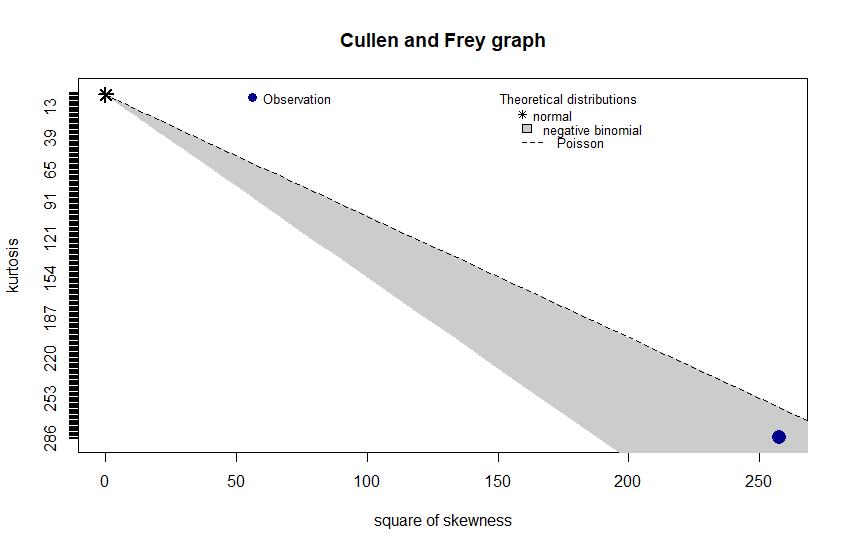
\includegraphics[width = 0.8\textwidth]{cf_norge.png}
    \caption{The Cullen and Frey graph for Norway}
    \label{cf_norge}
\end{figure}
Next, a negative binomial distribution, a normal distribution, and a Poisson distribution are fitted to the data using the maximum likelihood method. The negative binomial fits for both countries can be seen in Figure~\ref{fitNegbinomGermany} and Figure~\ref{fitNegbinomNorway}. The fits for the normal and Poisson distribution for both countries, are shown in the Appendix in Figure~\ref{fitNormalGermany}, Figure~\ref{fitPoissonGermany}, Figure~\ref{fitNormalNorway} and Figure~\ref{fitPoissonNorway}. \\
The QQ-plot for Germany and Norway looks quite similar, as there appears to be a linear relationship between the theoretical quantile and the sample quantiles, up to a certain point where the sample quantiles have a higher value than the theoretical quantiles, indicating that the distribution is right skewed. Since there are many municipalities with relatively few cases and few municipalities with a large number of cases, this is to be expected.
% \begin{figure}[H]
%     \centering
%     \includesvg[width = 0.8\textwidth]{fit_nbinom_germany.svg}
%     \caption{A negative binomial fit to the number of cases in German municipalities}
%     \label{fitNegbinomGermany}
% \end{figure}
\begin{figure}[H]
    \centering
    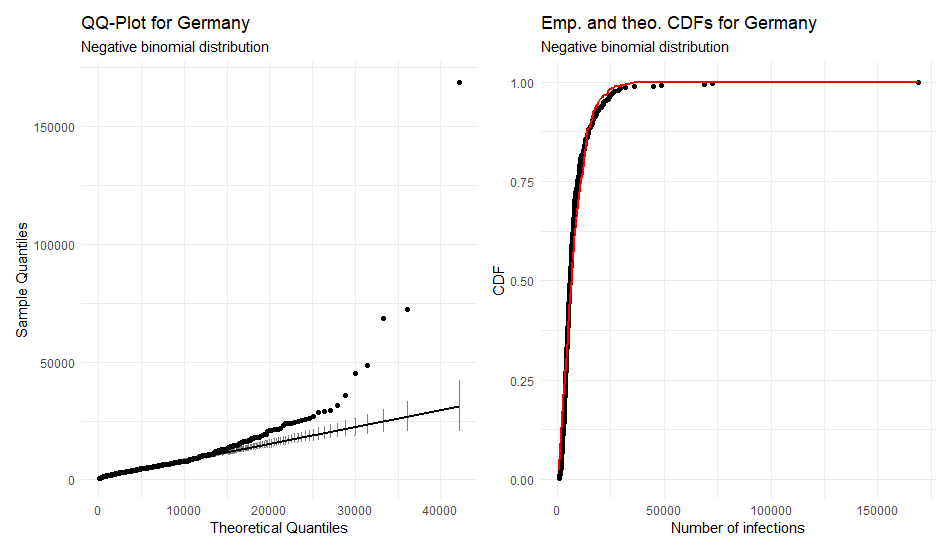
\includegraphics[width = 0.8\textwidth]{fit_nbinom_germany.png}
    \caption{A negative binomial fit to the number of cases in German municipalities}
    \label{fitNegbinomGermany}
\end{figure}
% \begin{figure}[H]
%     \centering
%     \includesvg[width = 0.8\textwidth]{fit_nbinom_norway.svg}
%     \caption{A negative binomial fit to the number of cases in Norwegian municipalities}
%     \label{fitNegbinomNorway}
% \end{figure}
\begin{figure}[H]
    \centering
    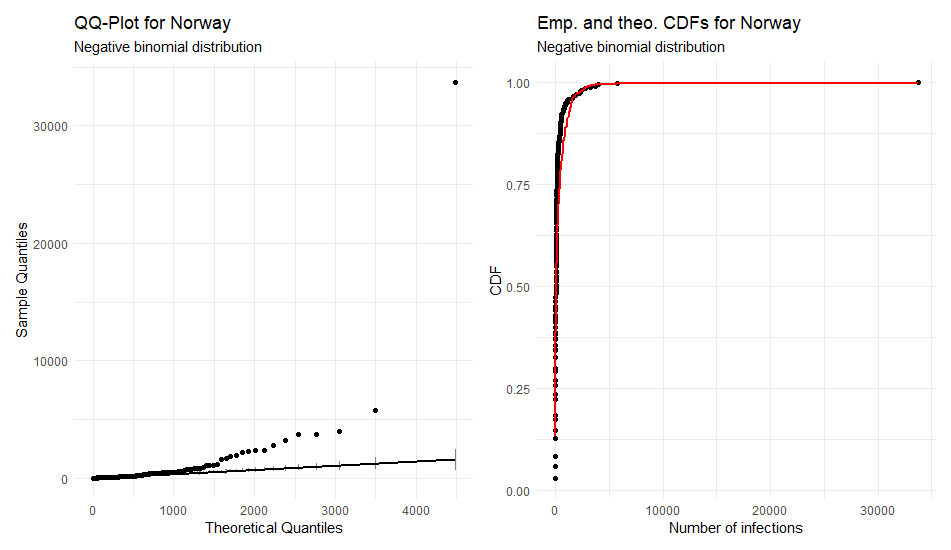
\includegraphics[width = 0.8\textwidth]{fit_nbinom_norway.png}
    \caption{A negative binomial fit to the number of cases in Norwegian municipalities}
    \label{fitNegbinomNorway}
\end{figure}
Lastly, the AIC was calculated for fitting a normal distribution to the data, a Poisson distribution to the data and a negative binomial distribution to the data. The values can be seen in Table~\ref{aic}. Afterwards, the negative binomial distribution was chosen as the distribution of the target variable in both cases. \\
\begin{table}[H] 
\caption{The AIC for different distributions for Germany and Norway \label{aic}}
\begin{tabular}{l l r}
\toprule
\textbf{Country}	& \textbf{Distribution}	& \textbf{AIC} \\
\midrule
Germany & Normal & 8360 \\
Germany & Poisson & 2148100 \\
Germany & Negative Binomial & 7731 \\
Norway & Normal & 6166 \\
Norway & Poisson & 366181 \\
Norway & Negative Binomial & 4086 \\
\bottomrule
\end{tabular}
\end{table} 
The poor fit for the Poisson distribution can be explained by looking at the range of the number of confirmed cases in a given municipality. For Germany, this number ranges from 508 to 137634 (as of March 18, 2021), while for Norway, the number ranges from 0 to 24905 (as of March 20, 2021). This results in a mean and standard deviation for Germany of 6617 and 9014, respectively. For Norway, the values for these metrics are 236 and 1389.
\subsection{Spatial Models for Germany}
First, a look is taken at the spatial models calculated for Germany. These models are based on data from 24 March 2021, when 2.695.037 people in Germany were confirmed infected with Covid-19. The five municipalities with the most infections are shown in Table~\ref{top5germany}.
\begin{table}[H] 
\caption{The municipalities with the most infections as of March 24th 2021. \label{top5germany}}
\begin{tabular}{l r r}
\toprule
\textbf{Municipality}	& \textbf{Population}	& \textbf{Number of infections} \\
\midrule
SK Berlin & 3644826 & 141639   \\     
SK Hamburg & 1841179 & 58661   \\
SK Munich & 1471508 & 57690   \\
SK Cologne & 1085664 & 37592   \\
Region Hannover & 1157624 & 36241   \\
\bottomrule
\end{tabular}
\end{table}
\subsubsection{Demographic Models}\label{sssec:demoGermany}
The model with the best performance based on the demographic variables was a Leroux model computed using the formula in Listing~\ref{codeDemoGermany}. The variables used for this model were the percentages of the vote for the six biggest German political parties. \\
The performance measures of this model and the best-performing BYM2 and Besag proper models are shown in Table~\ref{demoGermany}. 
\begin{table}[H] 
\caption{The performance measures for the best performing demographic model of each type. \label{demoGermany}}
\begin{tabular}{l r r r r}
\toprule
\textbf{Model}	& \textbf{DIC}	& \textbf{WAIC} & \textbf{CPO} & \textbf{MAE}\\
\midrule
Besag  & 4761 & 4712 & -2744 &  225675 \\
BYM2 & 4636 & 4617  & -2723 &  225255\\
Leroux & 4734  & 4749 & -3002 & 221620\\
No Spatial & 5538  & 5539 & -2769 & 223145\\
\bottomrule
\end{tabular}
\end{table}
The summary of the fixed effects is shown in Table~\ref{fixedDemoGermany}. To compute the posterior mean of the coefficients, the code shown in Listing~\ref{codePosteriorMean} can be used. \\
To get the expected value given a marginal function $\pi\left(x\right)$, the expected value of a function $f\left(x\right)$ is calculated, i.e.
\begin{equation*}
    \int f\left(x\right)\pi\left(x\right)dx.
\end{equation*}
To obtain a credibility interval of the fixed effects on the transformed scale, the code in Listing~\ref{codeCredibility} can be used. \\
\begin{table}[H] 
\caption{The fixed effects for the Leroux model. Values are rounded. A $^*$ denotes a significant effect.\label{fixedDemoGermany}}
\begin{tabular}{l r r r r c}
\toprule
\textbf{Variable}	& \textbf{Mean}	& \textbf{exp(mean$_{\hbox{p}}$)} & \textbf{exp(q0025$_{\hbox{p}}$)} & \textbf{exp(q0975$_{\hbox{p}}$)} & \textbf{sig.}\\
\midrule
(Intercept) & -0.08413 & 0.9194 & 0.8892 & 0.9503 &\\
afd & 0.1523 & 1.167& 1.016 & 1.334 &$^*$\\
FDP & -0.08350 & 0.9919& 0.9543 & 1.030 &\\
Gruene & -0.1029 & 0.9046 & 0.7831 & 1.039 &\\
Union & -0.1293 & 0.8817& 0.7486 & 1.031 &\\
SPD & -0.1510 & 0.8606 & 0.7901 & 0.9355 &\\
die\_linke & -0.2077 & 0.8133 & 0.7416 & 0.8898 &\\
\bottomrule
\end{tabular}
\end{table}
The posterior mean of the exponentiated intercept implies a -8.1\% risk rate across Germany with a credibility interval ranging from -11.1\% to -5.0\%. However, this coefficient is not significant. \\
This summary shows that especially people who come from regions where the AfD gets a higher share of the vote have a higher risk of contracting Covid-19. In Figure~\ref{sirgermany}, regions in eastern Germany often had a higher SIR. These are also the regions where the AfD tends to perform better in elections. The connection between the two can be attributed to the fact that the AfD is a right-wing party that openly criticises the measures taken to prevent the spread of the coronavirus. As a result, a large proportion of people who vote for the AfD do not take the measures seriously either and refuse to keep a safe distance or wear a mask in public spaces. \\
Wondreys and Mudde took a look at right-wing parties' responses to the pandemic, pointing out that while these parties were quick to warn about the virus, once cases spiked they criticised the measures taken to contain the spread of the virus. They also noted that right-wing parties supported demonstrations against these measures. However, they also stressed that these parties often rejected the measures proposed by the leading parties because they themselves were part of the opposition, as is the case with the AfD in Germany \cite{wondreys2020victims}.  \\
Farias and Pilati also conducted a study in Brazil to predict social distancing violation intention and past non-compliance during the COVID-19 pandemic, controlling for the effects of intolerance of uncertainty and sociodemographic variables. Their results included that individuals who support right-wing parties are more likely to violate social distancing measures \cite{farias2020violating}. \\
An increase by one standard deviation for the AfD leads to a risk increase of about 16.7\%. No significant effects were observed for all other parties. \\
It is interesting, however, that the party "Die Linke", which is currently the most left-wing party in the German parliament, has the smallest posterior mean. \\
As this was the overall best-performing spatial model for Germany, a look is taken at the posterior means $\pmb{\zeta} = \exp{\left(\xi\right)}$ of the area-specific risks. Since the uncertainty associated with them can also be mapped, the posterior probability $\mathbb{P}\left(\zeta_i > 1|\pmb{y}\right)$ is visualised as well. In Figure~\ref{posteriorGermany}, it can be seen that the relative risk is above 1 for large parts of Germany, except for most of northern Germany and some parts in the south of the country. The posterior probability is highest for parts of North Rhine-Westphalia, home to Germany's most populous metropolitan area, the Ruhr area, and for Saxony and Thuringia, both political strongholds of the AfD. The higher numbers in Bavaria can be explained by the large common borders with Austria and the Czech Republic, two countries that were more affected by the pandemic. Many people cross these borders because of tourism and many guest workers come from the Czech Republic to work on agricultural land in Bavaria, which resulted in several Covid-19 outbreak events.
\begin{figure}[H]
    \centering
    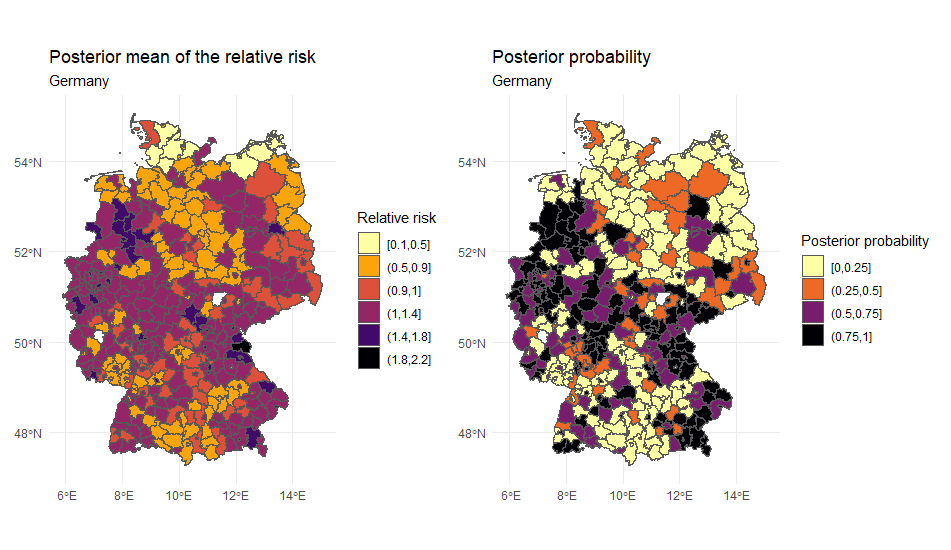
\includegraphics[width = \textwidth]{posterior_germany.png}
    \caption{Posterior mean of the area-specific risk and the posterior probability.}
    \label{posteriorGermany}
\end{figure}
% \begin{figure}[H]
%     \centering
%     \includesvg[width = textwidth]{posterior_germany.svg}
%     \caption{A negative binomial fit to the number of cases in Norwegian municipalities}
%     \label{nb_norge}
% \end{figure}
Compared to the standardised incidence rate in Germany, shown in Figure~\ref{sirgermany}, it can be seen that the parts of Germany with the lowest SIR, Northern Germany, are also the parts of Germany with the lowest relative risk. Saxony had the highest SIR and also has an increased relative risk. Most parts of Germany that had an SIR of around 1 have a relative risk between 1 and 1.4.
\subsubsection{Infrastructure Models}\label{sssec:infraGermany}
When it comes to the models based on the infrastructural variables, a model without any spatial component performed the best. It was computed using formula in Listing~\ref{codeInfraGermany}. \\
The performance measures of this model and the best-performing other models are shown in Table~\ref{infraGermany}
\begin{table}[H] 
\caption{The performance measures for the best performing infrastructure model of each type. \label{infraGermany}}
\begin{tabular}{l r r r r}
\toprule
\textbf{Model}	& \textbf{DIC}	& \textbf{WAIC} & \textbf{CPO} & \textbf{MAE}\\
\midrule
Besag & 4753 & 4708 & -2772 & 225502\\
BYM2 & 4674 & 4664 & -2767 & 223208\\
Leroux & 4767 & 4787 & -3278 & 200001\\
No Spatial & 5655 & 5654 & -2847 & 189664\\
\bottomrule
\end{tabular}
\end{table}
The values of the covariates are shown in Table~\ref{fixedInfraGermany}.
\begin{table}[H] 
\caption{The fixed effects for the model without a spatial component. Values are rounded. A $^*$ denotes a significant effect.\label{fixedInfraGermany}}
\begin{tabular}{l r r r r c}
\toprule
\textbf{Variable}	& \textbf{Mean}	& \textbf{exp(mean$_{\hbox{p}}$)} & \textbf{exp(q0025$_{\hbox{p}}$)} & \textbf{exp(q0975$_{\hbox{p}}$)} & \textbf{sig.}\\
\midrule
(Intercept) & -0.02831 & 0.9723 & 0.9373 & 1.009 &\\
bakeries & 0.5143 & 1.683 & 1.351 & 2.074 &$^*$\\
pop\_dens & 0.1089 & 1.116 & 1.049 & 1.187 & $^*$\\
place\_of\_ & \multirow{2}{*}{0.09044} & \multirow{2}{*}{1.095} & \multirow{2}{*}{1.033} & \multirow{2}{*}{1.160} &\multirow{2}{*}{$^*$}\\
worship &  \\
higher\_ & \multirow{2}{*}{0.008236} & \multirow{2}{*}{1.009} & \multirow{2}{*}{0.9536} & \multirow{2}{*}{1.069} &\\
education \\
nursing\_home & 0.006448 & 1.007 & 0.9602 & 1.057 &\\
entertainment & -0.01045 & 0.9936 & 0.8311 & 1.180 &\\
platform & -0.01408 & 0.9868 & 0.9147 & 1.064 &\\
aerodrome & -0.01525 & 0.9850 & 0.9541 & 1.020 &\\
sport & -0.06345 & 0.9401 & 0.8371 & 1.053 \\
schools & -0.08823 & 0.9178 & 0.7980 & 1.051 &\\
retail & -0.1295 & 0.8792 & 0.8128 & 0.9524 &\\
kindergarten & -0.1346 & 0.8805 & 0.6907 & 0.9524 &\\
hairdresser & -0.1401 & 0.8752 & 0.6925 & 1.092 &\\
restaurant & -0.1757 & 0.8425 & 0.6995 & 1.008 &\\
\bottomrule
\end{tabular}
\end{table}
Findings from these results are that bakeries, places of worship and population density increase the risk of infection. For bakeries, an increase of 1 standard deviation leads to a risk increase of 68.3\%. Bakeries are relatively widespread in Germany and many people go there several times a week to get fresh bread or other baked goods. When many people congregate in bakeries, viruses can spread more easily. \\
A 1 standard deviation increase in population density leads to an 11.6\% increase in relative risk, which should not be too surprising since in communities with higher population density, people come into contact with more people, which in turn helps the virus move from host to host. \\
Finally, places of worship were not closed for a long time in Germany due to freedom of religion and therefore people gathered in churches, mosques and the like. A 1 standard deviation increase in these places of worship therefore leads to a 9.5\% increase in the risk of contracting Covid-19. \\
Yezli and Khan's paper argues for the closure of these places of worshipon the grounds that they pose a risk of transmitting COVID-19 to potentially large numbers of people through a single case. Gatherings at these places often involve dense mixing of many people in a confined space, sometimes for long periods of time \cite{yezli2020covid}.
\subsubsection{Combined Models}
Finally, models are considered that include both the infrastructural and demographic covariates. Due to the amount of variables, all models run are based on variable selection. \\
The best performing model was again a model with no spatial component, computed with the formula shown in Listing~\ref{codeBothGermany}. \\
The performance measures of the computed models are shown in Table~\ref{allGermany}.
\begin{table}[H] 
\caption{The performance measures for the best performing demographic + infrastructure model of each type. \label{allGermany}}
\begin{tabular}{l r r r r}
\toprule
\textbf{Model}	& \textbf{DIC}	& \textbf{WAIC} & \textbf{CPO} & \textbf{MAE}\\
\midrule
Besag&  4806 & 4739 & -2711 & 362281\\
BYM2 & 4665 & 4651 & -2704 & 350752\\
Leroux & 5020 & 5022 & -2882 & 280649 \\
No Spatial & 5423 & 5423 & -2721 & 273879 \\
\bottomrule
\end{tabular}
\end{table}
The fixed effects are shown in Table~\ref{fixedAllGermany}.

\begin{table}[H] 
\caption{The fixed effects for the model without a spatial component. Values are rounded. A $^*$ denotes a significant effect.\label{fixedAllGermany}}
\begin{tabular}{l r r r r c}
\toprule
\textbf{Variable}	& \textbf{Mean}	& \textbf{exp(mean$_{\hbox{p}}$)} & \textbf{exp(q0025$_{\hbox{p}}$)} & \textbf{exp(q0975$_{\hbox{p}}$)} & \textbf{sig.}\\
\midrule
(Intercept) & -0.0712 & 0.9314 & 0.9047 & 0.9589 \\
unemployed\_ & \multirow{2}{*}{0.6614} & \multirow{2}{*}{1.954} & \multirow{2}{*}{1.506} & \multirow{2}{*}{2.492} & \multirow{2}{*}{$^*$}\\
foreigners \\
afd & 0.2023  & 1.225 & 1.147 & 1.308 & $^*$\\
pop\_dens & 0.1245 & 1.133 & 1.072 & 1.197 & $^*$\\
shops & 0.1234 & 1.143 & 0.8593 & 1.489 \\
schools & 0.1177 &1.127 & 1.002 & 1.264 & $^*$\\
kindergarten & 0.07769 & 1.085 & 0.9052 & 1.292 \\
sex & 0.06440 &1.067 & 1.031 & 1.103 & $^*$\\
higher\_ & \multirow{2}{*}{0.06279} & \multirow{2}{*}{1.065} & \multirow{2}{*}{1.021} & \multirow{2}{*}{1.111} & \multirow{2}{*}{$^*$} \\
education & \\
entertainment & 0.04197 & 1.046 & 0.9073 & 1.120 \\
clinic & 0.03603&  1.037 & 0.9609 & 1.120 \\
sport & 0.03435& 1.036 & 0.9478 & 1.130 \\
platform & 0.01969 &  1.020 & 0.9581 & 1.086 \\
log & \multirow{2}{*}{0.01426} & \multirow{2}{*}{1.015} & \multirow{2}{*}{0.9776} & \multirow{2}{*}{1.051} \\
income\_total\\
place\_of\_ & \multirow{2}{*}{0.01288} & \multirow{2}{*}{1.013} & \multirow{2}{*}{0.9646} & \multirow{2}{*}{1.064} \\
worship\\
protection\_ & \multirow{2}{*}{0.01186} & \multirow{2}{*}{1.015} & \multirow{2}{*}{0.8636} & \multirow{2}{*}{1.185} \\
seekers\\
aerodrome & 0.0004896 & 1.006 & 0.9766 & 1.027 \\
nursing\_home & -0.002786 & 0.9974 & 0.9636 & 1.032 \\ 
FDP & -0.01863 & 0.9817 & 0.9464 & 1.018 \\
retail & -0.01983 & 0.9809 & 0.9179 & 1.048 \\
log & \multirow{2}{*}{-0.03577} & \multirow{2}{*}{0.9650} & \multirow{2}{*}{0.9362} & \multirow{2}{*}{0.9940} \\
trade\_tax \\
log & \multirow{2}{*}{-0.4560} & \multirow{2}{*}{0.9557} & \multirow{2}{*}{0.9152} & \multirow{2}{*}{0.9973} \\
income\_tax \\
welfare\_ & \multirow{2}{*}{-0.07744} & \multirow{2}{*}{0.9277} & \multirow{2}{*}{0.8096} & \multirow{2}{*}{1.058} \\
recipients &  \\
bakeries & -0.07973 & 0.9273 & 0.7711 & 1.105 \\
office & -0.1081 & 0.8985 & 0.8175 & 0.9855 \\
SPD & -0.1100 & 0.8959 & 0.8668 & 0.9259 \\
die\_linke & -0.1627 & 0.8502 & 0.8043 & 0.8980 \\
restaurant & -0.1939 & 0.8262 & 0.7092 & 0.9576 \\
Gruene & -0.1943 & 0.8239 & 0.7726 & 0.8775 \\
unemployed\_ & \multirow{2}{*}{-0.6720} & \multirow{2}{*}{0.5163} & \multirow{2}{*}{0.3827} & \multirow{2}{*}{0.6818} \\
total & \\
\bottomrule
\end{tabular}
\end{table}
According to this model, the three biggest driving factors for the number of infections are the amount of unemployed foreigners, the share of the vote for the AfD and the population density. The influence of the AfD was already discussed in Section~\ref{sssec:demoGermany}, only in this case an increase of 1 standard deviation leads to a risk increase of 22.5\%. In Section~\ref{sssec:infraGermany} population density was discussed. Here, a 1 standard deviation increase leads to a 13.3\% increase in relative risk. For unemployed foreigners, a 1 standard deviation increase leads to a 95.4\% increase in risk. \\
Other factors that positively influence the risk of infection are the number of schools, the proportion of women in the population and the number of higher educational institutions. A 1 standard deviation increase in the number of schools leads to a 12.7\% increase in risk, which could be an indicator that schools should remain closed because so many children from different households meet there, providing a good place for a virus to spread. Schools in Germany actually closed relatively late, and did reopen at the beginning of 2021.\\
A 1 standard deviation increase in the proportion of women leads to a 6.7\% increase in risk and for higher education buildings a 1 standard deviation increase leads to a 6.5\% increase in risk. 
\subsection{Spatial Models for Norway}
Next, the same types of models are evaluated for Norway. These models are based on data from 24 March 2021, when 87537 people in Norway were confirmed infected with Covid-19. The five municipalities with the most infections are shown in Table~\ref{top5norway}.
\begin{table}[H] 
\caption{The municipalities with the most infections as of March 24th 2021. \label{top5norway}}
\begin{tabular}{l r r}
\toprule
\textbf{Municipality}	& \textbf{Population}	& \textbf{Number of infections} \\
\midrule
Oslo & 693494 & 26151 \\
Bergen & 283929 & 4738 \\
Drammen & 101386 & 3149 \\
Bærum & 127731 & 2834 \\
Lillestrøm & 85983 & 2779 \\
\bottomrule
\end{tabular}
\end{table}
\subsubsection{Demographic Models}\label{sssec:demoNorway}
The best demographic model was a model without any spatial component calculated using the formula shown in Listing~\ref{codeDemoNorway}. \\
The performance measures for all four models are shown in Table~\ref{demoNorway}. It is noticeable that the mean error in Norway is significantly smaller, suggesting that the models for Germany have greatly overestimated or underestimated the number of infections.
\begin{table}[H] 
\caption{The performance measures for the best performing demographic model of each type. \label{demoNorway}}
\begin{tabular}{l r r r r}
\toprule
\textbf{Model}	& \textbf{DIC}	& \textbf{WAIC} & \textbf{CPO} & \textbf{MAE}\\
\midrule
Besag  & 2396 & 2403 & -4369 & 10149 \\
BYM2 & 2224 & 2202 & -6793 & 10002\\
Leroux & 2225  & 2192 & -6810 & 8460\\
No Spatial & 2696  & 2702 & -1376 & 7710\\
\bottomrule
\end{tabular}
\end{table}
All other performance measures for these models are also lower than for the models computed for Germany. \\
The effects of the covariates are shown in Table~\ref{fixedDemoNorway}.
\begin{table}[H] 
\caption{The fixed effects for the model without a spatial component. Values are rounded. A $^*$ denotes a significant effect.\label{fixedDemoNorway}}
\begin{tabular}{l r r r r c}
\toprule
\textbf{Variable}	& \textbf{Mean}	& \textbf{exp(mean$_{\hbox{p}}$)} & \textbf{exp(q0025$_{\hbox{p}}$)} & \textbf{exp(q0975$_{\hbox{p}}$)} & \textbf{sig.}\\
\midrule
(Intercept) & -0.7857 & 0.4563 & 0.4151 & 0.5015 & \\
unemp\_total & 0.3785 & 1.466 & 1.229 & 1.738 & $^*$\\
unemp\_immg & 0.1284 & 1.141 & 0.9752 & 1.334 & \\
\bottomrule
\end{tabular}
\end{table}
The only significant influence on the number of infections is the total number of unemployed people in a municipality. A 1 standard deviation increase in total unemployment leads to a 46.6\% increase in the risk. A possible explanation for this could be that the unemployed spend less time at home and instead move around more and thus have more contact with people, but this should be taken with a grain of salt.
\subsubsection{Infrastructure Models}
For the models based on the infrastructure variables, the best predictive performance was again observed for a model without a spatial component. The formula is shown in Listing~\ref{codeInfraNorway}. \\
The performance measure for the models is shown in Table~\ref{infraNorway}.
\begin{table}[H] 
\caption{The performance measures for the best performing infrastructure model of each type. \label{infraNorway}}
\begin{tabular}{l r r r r}
\toprule
\textbf{Model}	& \textbf{DIC}	& \textbf{WAIC} & \textbf{CPO} & \textbf{MAE} \\
\midrule
Besag  & 2326 & 2335 & -8405 & 11694 \\
BYM2 & 2218 & 2187 & -6532 & 11866\\
Leroux &  2230 & 2167 & -7128 & 12943\\
No Spatial & 2711 & 2716 & -1594 & 11094 \\
\bottomrule
\end{tabular}
\end{table}
The effect of the covariates are shown in Table~\ref{fixedInfraNorway}.
\begin{table}[H] 
\caption{The fixed effects for the model with no spatial component. Values are rounded. A $^*$ denotes a significant effect.\label{fixedInfraNorway}}
\begin{tabular}{l r r r r c}
\toprule
\textbf{Variable}	& \textbf{Mean}	& \textbf{exp(mean$_{\hbox{p}}$)} & \textbf{exp(q0025$_{\hbox{p}}$)} & \textbf{exp(q0975$_{\hbox{p}}$)} & \textbf{sig.}\\
\midrule
(Intercept) & -0.7717 & 0.4628 & 0.4204 & 0.5094 &\\
pop\_dens & 0.5154 & 1.688 & 1.318 & 2.181 & $^*$ \\
schools & 0.4272 & 1.577 & 0.9724 & 2.458 & \\
kindergarten & 0.2583 & 1.317 & 0.9140 & 1.868 \\
nursing\_home & 0.03801 & 1.040 & 0.9542 & 1.152 \\
place\_of\_ & \multirow{2}{*}{-0.08318} & \multirow{2}{*}{0.9324} & \multirow{2}{*}{0.0.6746} & \multirow{2}{*}{1.270} & \multirow{2}{*}{}\\
worship\\
office &-0.1311 & 0.8819 & 0.7206 & 1.082\\
restaurant & -0.2211 & 0.8448 & 0.4220 & 1.501 & \\
shops & -0.5423 &0.6579 & 0.2214 & 1.541 & \\
\bottomrule
\end{tabular}
\end{table}
Again, only one significant effect was observed, the population density. A 1 standard deviation increase leads to a risk increase of 68,8\%. The effect of the population density  has already been discussed in Section~\ref{sssec:infraGermany}
\subsubsection{Combined Models}
For the models containing variables related to the demographic of Norway and the infrastructure, again a Besag model performed the best. Its formula can be seen in Listing~\ref{codeBothNorway}. \\
The performance measures for the models are shown in Table~\ref{bothNorway}
\begin{table}[H] 
\caption{The performance measures for the best performing demographic + infrastructure model of each type. \label{bothNorway}}
\begin{tabular}{l r r r r}
\toprule
\textbf{Model}	& \textbf{DIC}	& \textbf{WAIC} & \textbf{CPO} & \textbf{MAE} \\
\midrule
Besag  & 2395 & 2402 & -5000 & 13111 \\
BYM2 & 2215 & 2184 & -6406 & 13932\\
Leroux &  2229 & 2193 & -7677 & 14841\\
No Spatial & 2676 & 2682 & -1532 & 13479 \\
\bottomrule
\end{tabular}
\end{table}
The fixed effects are shown in Table~\ref{fixedAllNorway}.
\begin{table}[H] 
\caption{The fixed effects for the Besag model. Values are rounded. A $^*$ denotes a significant effect.\label{fixedAllNorway}}
\begin{tabular}{l r r r r c}
\toprule
\textbf{Variable}	& \textbf{Mean}	& \textbf{exp(mean$_{\hbox{p}}$)} & \textbf{exp(q0025$_{\hbox{p}}$)} & \textbf{exp(q0975$_{\hbox{p}}$)} & \textbf{sig.}\\
\midrule
(Intercept) & -1.055 & 0.3534 & 0.2464 & 0.4885 &\\
construction\_ & \multirow{2}{*}{0.1905} & \multirow{2}{*}{1.239} & \multirow{2}{*}{0.7927} & \multirow{2}{*}{1.853}  \\
pt\_work \\
clinic & 0.1735 & 1.252 & 0.6368 & 2.226 \\
pop\_dens & 0.1717 & 1.194 & 0.9701 & 1.456 \\
unemp\_tot & 0.1583 & 1.173 & 1.058 & 1.297 & $^*$\\
schools & 0.1068 & 1.127 & 0.8121 & 1.529 &\\
sex & 0.04749 & 1.050 & 0.9453 & 1.163 \\
restaurant & 0.03536 & 1.085 & 0.5718 & 1.873\\
higher\_& \multirow{2}{*}{-0.06041} & \multirow{2}{*}{0.9434} & \multirow{2}{*}{0.8270} & \multirow{2}{*}{1.070}\\
education\\
median\_age & -0.1117 & 0.8957 & 0.8034 & 0.9950 & \\
workers\_ft\_ & \multirow{2}{*}{-0.5226} & \multirow{2}{*}{0.6396} & \multirow{2}{*}{0.2753} & \multirow{2}{*}{1.264} \\
work\\
\bottomrule
\end{tabular}
\end{table}
Again, only 1 significant effect was found, again the total number of unemployed people. This time, a 1 standard deviation increase leads to a risk increase of 17.3\%, which seems to be a more reasonable figure than the one from the demographic model in Section~\ref{sssec:demoNorway}. \\
Looking at the posterior mean relative risk, it can be seen that the region in and around the capital Oslo is most at risk, as the posterior mean of the relative risk can be as high as 6, with a posterior probability between 0.75 and 1. In addition, some municipalities around Bergen and Ulvik are also more at risk, with a relative risk of up to 3.4 and a posterior probability between 0.75 and 1. \\
The risk seems to be lowest in the parts north of Trondheim and south of Bodø, where the relative risk is mostly below 1. For many municipalities in Troms og Finnmark, the northernmost part of Norway, the posterior mean is also below 1, but for a few regions it is above 1 with posterior probabilities between 0.5 and 0.75 and 0.75-1.
\begin{figure}[H]
    \centering
    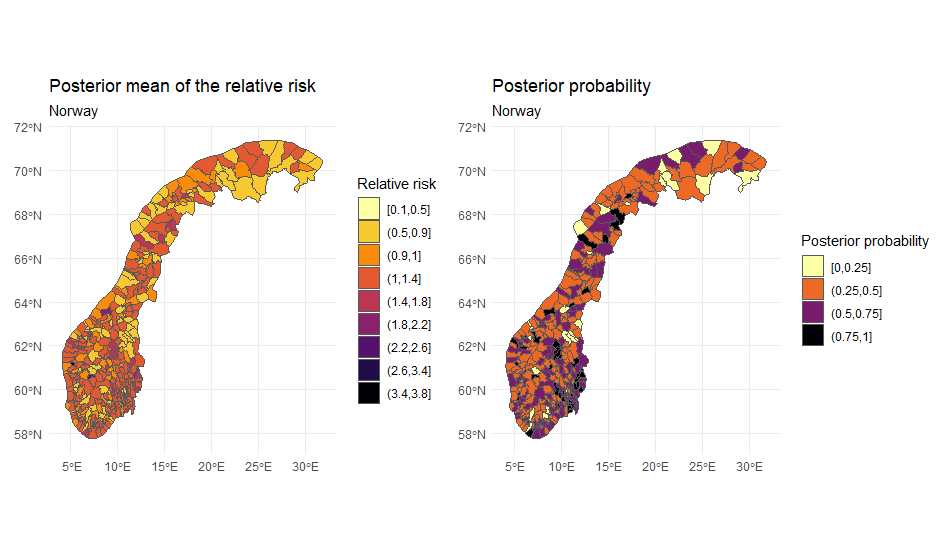
\includegraphics[width = \textwidth]{posterior_norway.png}
    \caption{Posterior mean of the area-specific risk and the posterior probability.}
    \label{posteriorNorway}
\end{figure}
% \begin{figure}[H]
%     \centering
%     \includesvg[width = \textwidth]{posterior_norway.svg}
%     \caption{Posterior mean of the area-specific risk and the posterior probability.}
%     \label{posteriorNorway}
% \end{figure}
For better interpretability, the logarithmic posterior mean is shown in Figure~\ref{posteriorNorwayLog}.
\begin{figure}[H]
    \centering
    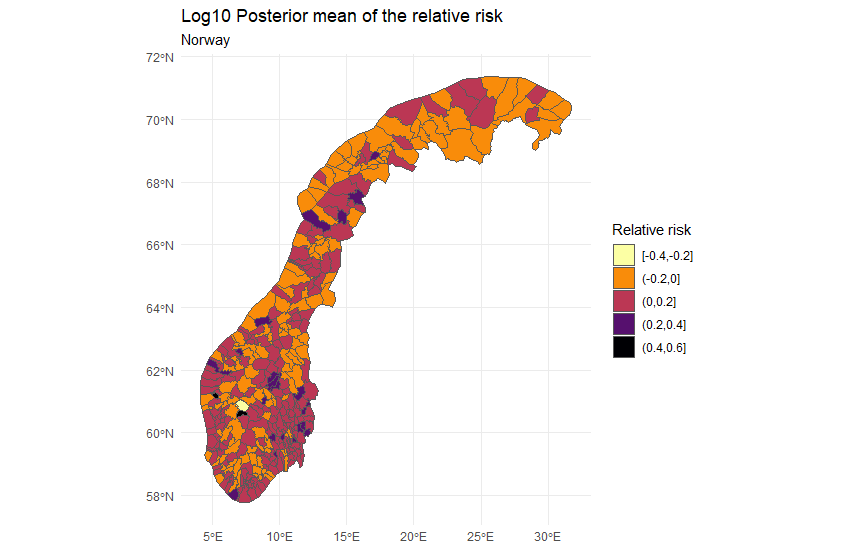
\includegraphics[width = \textwidth]{posterior_norway_log.png}
    \caption{Logarithmic posterior mean of the area-specific risk.}
    \label{posteriorNorwayLog}
\end{figure}
% \begin{figure}[H]
%     \centering
%     \includesvg[width = \textwidth]{posterior_norway_log.svg}
%     \caption{Logarithmic posterior mean of the area-specific risk.}
%     \label{posteriorNorwayLog}
% \end{figure}
Comparing the log relative risk with the log standardised incidence ratio in Figure~\ref{sirnorwaylog}, these two are quite similar. For most parts of Norway, the risk is at or below 0, while there is an increased risk in the Oslo region. However, there are a few municipalities that have a log-standardised incidence ratio of about 0, but a higher log-relative risk than this. Most of these are located in southern Norway, but a few are scattered throughout the rest of the country.
\clearpage
\subsection{Choice of Prior Sensitivity}
As can be seen in equation~\ref{pcprec}, there is flexibility when it comes to choosing the values for the standard deviation $\sigma_0$ as well as the probability $\alpha$. Therefore, an upper bound for the standard deviation can be chosen as well as the weight placed on this "tail event", describing how informative the resulting prior is. In the following, an assessment is made of how the performance of a Besag model, a BYM2 model and a Leroux model changes when playing around with these two values.
\subsubsection{Changing the Value for the Standard Deviation}
By allowing the precision to be greater, the variance is forced to be smaller. Hence, choosing a higher value for the precision leads to lower values for the DIC, WAIC and CPO, as can be seen in Figure~\ref{comparison_norway_1} and Figure~\ref{comparison_norway_2}. While this indicates a better fit to the training data, Figure~\ref{comparison_norway_2} also shows that the MAE increases when a higher value for $U=\sigma_0$ is chosen, as the models overfit on the training data and therefore make worse predictions. \\
The corresponding figures for Germany are shown in Figure~\ref{comparison_germany_1} and Figure~\ref{comparison_germany_2} in the Appendix.
\begin{figure}[H]
    \centering
    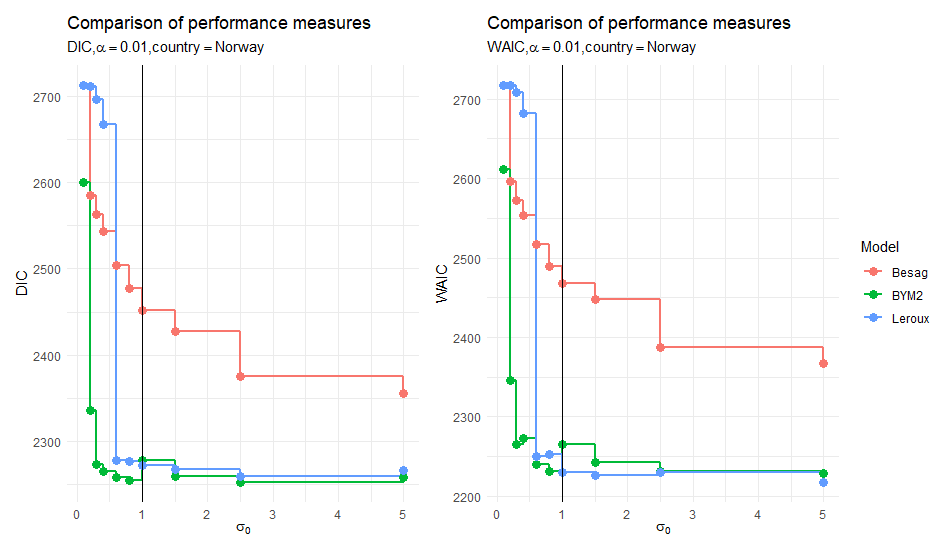
\includegraphics[width = \textwidth]{comparison_1_norway.png}
    \caption{Value of the DIC and WAIC when changing the value for $\sigma_0$. The black line highlights the values for $\sigma_0$ = 1.}
    \label{comparison_norway_1}
\end{figure}
% \begin{figure}[H]
%     \centering
%     \includesvg[width = \textwidth]{comparison_1_norway.svg}
%     \caption{Value of the DIC and WAIC when changing the value for $\sigma_0$. The black line highlights the values for $\sigma_0$ = 1.}
%     \label{comparison_norway_1}
% \end{figure}
\begin{figure}[H]
    \centering
    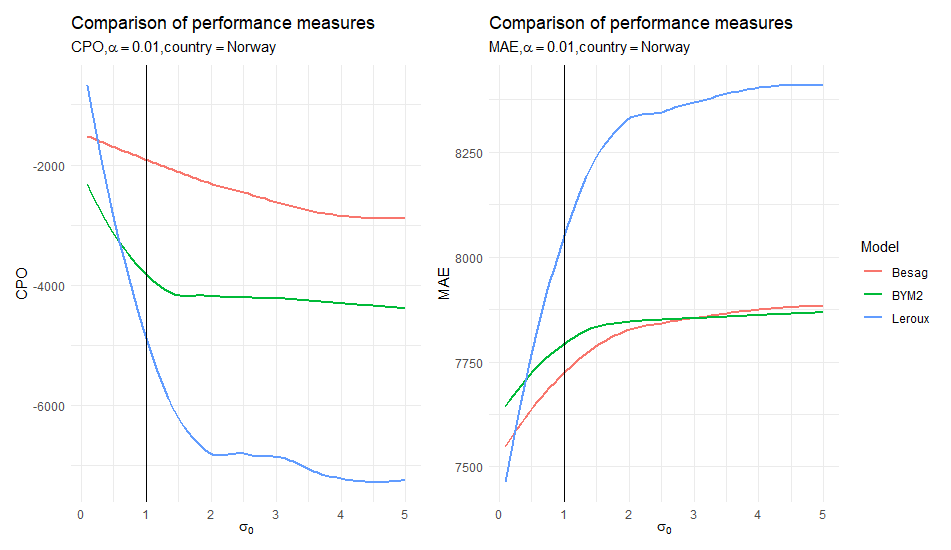
\includegraphics[width = \textwidth]{comparison_2_norway.png}
    \caption{Value of the CPO and MAE when changing the value for $\sigma_0$. The black line highlights the values for $\sigma_0$ = 1.}
    \label{comparison_norway_2}
\end{figure}
% \begin{figure}[H]
%     \centering
%     \includesvg[width = \textwidth]{comparison_2_norway.svg}
%     \caption{Value of the CPO and MAE when changing the value for $\sigma_0$. The black line highlights the values for $\sigma_0$ = 1.}
%     \label{comparison_norway_2}
% \end{figure}

\subsubsection{Changing the Value for the Probability}
By allowing the probability to be greater, the certainty with which the accuracy is 1 becomes less and it could therefore actually be greater than 1. Therefore, a trend similar to that seen in Figure~\ref{comparison_norway_1} and Figure~\ref{comparison_norway_2} can be seen. Choosing a higher value for the probability leads to lower values for the DIC, WAIC and CPO and a higher value for MAE, as can be seen in Figure~\ref{comparison_norway_3} and Figure~\ref{comparison_norway_4}. \\
The corresponding figures for Germany are shown in Figure~\ref{comparison_germany_3} and Figure~\ref{comparison_germany_4} in the Appendix.
\begin{figure}[H]
    \centering
    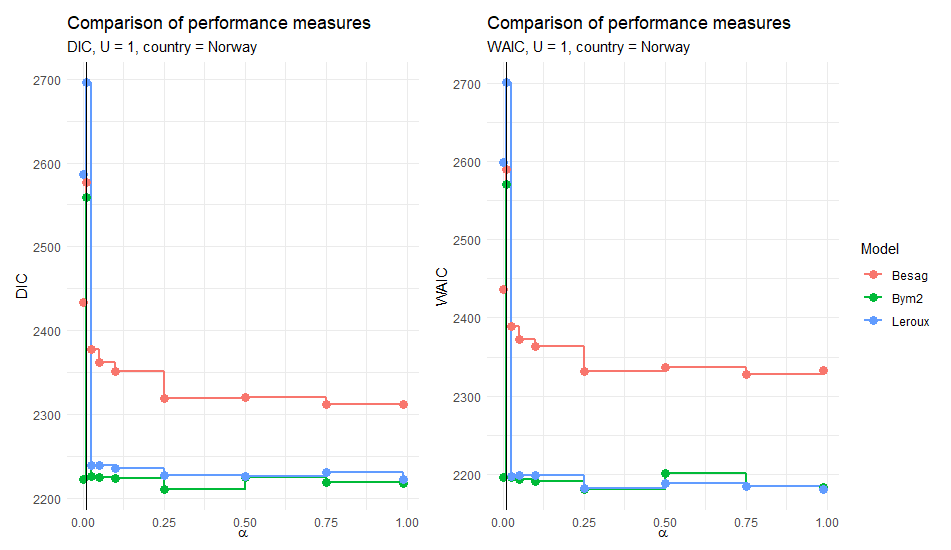
\includegraphics[width = \textwidth]{comparison_3_norway.png}
    \caption{Value of the DIC and WAIC when changing the value for $\alpha$. The black line highlights the values for $\alpha$ = 0.01.}
    \label{comparison_norway_3}
\end{figure}
% \begin{figure}[H]
%     \centering
%     \includesvg[width = \textwidth]{comparison_3_norway.svg}
%     \caption{Value of the DIC and WAIC when changing the value for $\alpha$. The black line highlights the values for $\alpha$ = 0.01.}
%     \label{comparison_norway_3}
% \end{figure}
\begin{figure}[H]
    \centering
    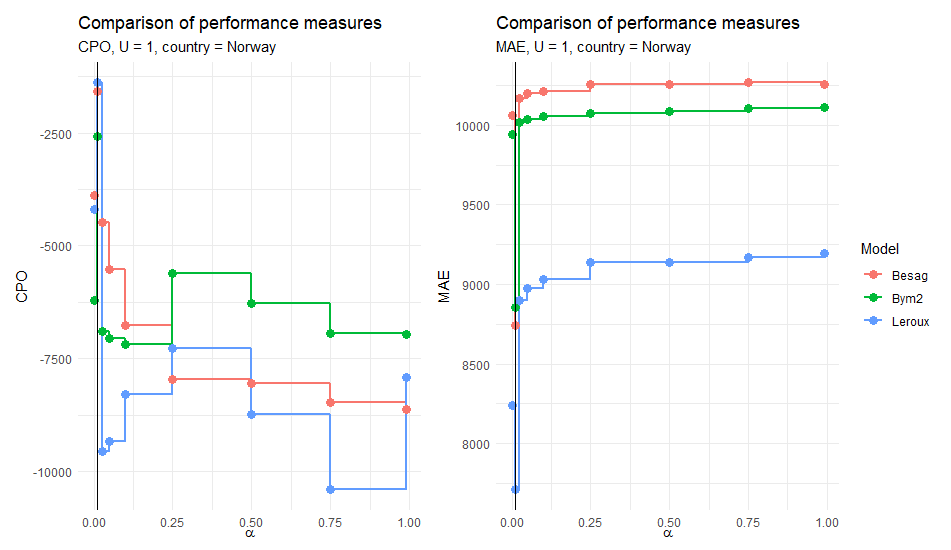
\includegraphics[width = \textwidth]{comparison_4_norway.png}
    \caption{Value of the CPO and MAE when changing the value for $\alpha$. The black line highlights the values for $\alpha$ = 0.01.}
    \label{comparison_norway_4}
\end{figure}
% \begin{figure}[H]
%     \centering
%     \includesvg[width = \textwidth]{comparison_4_norway.svg}
%     \caption{Value of the CPO and MAE when changing the value for $\alpha$. The black line highlights the values for $\alpha$ = 0.01.}
%     \label{comparison_norway_4}
% \end{figure}

\clearpage
\section{Spatio-Temporal Models}
\subsection{Spatio-Temporal Models for Germany}
\subsection{Spatio-Temporal Models for Norway}
\clearpage
\section{Predictive Models}
\subsection{Predictive Models for Germany}
\subsection{Predictive Models for Norway}
% !TEX root = ../my-thesis.tex
%
\chapter{Discussion}\label{sec:discussion}
After fitting models, the next step is to critically examine and evaluate the results. The evaluation of the spatial models follows a simple scheme. First, a brief look is taken at the models without the spatial component, before the spatial models are reviewed and compared with the non-spatial models. Next, it is examined which factors significantly influence the risk of infection and why these factors might have an impact. For this, the coefficient of the BYM2 model are analysed. Finally, a look at area-specific risk is taken to see which regions in a given country are most at risk.
\section{Discussion of the (Non)-Temporal Models}
\subsection{Discussion of the (Non)-Temporal Models for Norway}\label{sec:models_norway}
The non-spatial model for Norway identifies five significant effects:
\begin{itemize}
    \item The number of unemployed immigrants 
    \item The total number of immigrants 
    \item The urban density 
    \item The proportion of females 
\end{itemize}
Moreover, the intercept is significant. \\
Comparing the spatial models with the non-spatial models using Table~\ref{allNorway}, it can be seen that the BYM2, proper Besag and the non-spatial model perform almost equally well in terms of the DIC and WAIC, while the Leroux model performs best in terms of these two metrics. In terms of CPO, all spatial models perform better than the non-spatial model, with the Leroux model again performing best. However, the MAE shows that the non-spatial model has the best predictive performance, ahead of the proper Besag model, the BYM2 model and the Leroux model. This shows that the Leroux model overfits the training data more than the other models, a characteristic that can be seen in Figure~\ref{comparison_norway_1}. The fact that the non-spatial model performs better than the spatial models is an indication that the spatial effect in Norway is not strong and that a different class of models may be better suited to identify critical factors affecting infection rates. Table~\ref{fixedAllNorway_spatial} shows that adding the spatial effect did not suddenly cause any variables to become significant, while all variables, including the intercept, that are significant in the non-spatial model remain significant. Nevertheless, significant effects are found and have to be discussed. \\
The exponentiated intercept implies a risk rate of -59.1\% across Norway,which means that the risk of contracting Covid-19 in Norway is 40.9\%. Factors related to immigration play a crucial role in the relative risk of getting infected with Covid-19. A one standard deviation increase in the number of unemployed immigrants leads to a 22.6\% increase in risk and a one standard deviation increase in the total number of immigrants leads to a 22.8\% increase in risk. Unfortunately, there are no studies analysing the relationship between unemployed immigrants and the risk of contracting Covid-19, as studies mostly focus on the relationship between unemployment in general and the risk of disease. Unemployment, however, turns out to be non-significant in the BYM2 model. Looking at older studies, Elkeles and Seifert (1996) conducted a longitudinal study that looked at the unemployment status and health of labour migrants in Germany. They found that immigrants are often employed in jobs with higher health risks and stress and therefore had poorer health \autocite[][]{elkeles1996immigrants}. Sia et al. (2019) analysed the association between immigration status and unemployment and men's and women's health using data from the Canadian Health Measures Survey. The study provided evidence of biological associations between unemployment and the likelihood of common chronic diseases, inflammation and possible malnutrition, with unemployed immigrants, and particularly unemployed immigrant women, being more prone to chronic diseases \autocite[][]{sia2019chronic}. Thus, there is precedent for an association between unemployment and immigrants and a higher risk of disease, however, further research would need to be conducted to analyse the association between unemployed immigrants and the risk of Covid-19 infection. \\
The last factor that influences the relative risk is urban density, where an increase of 1 standard deviation leads to an increase in the relative risk of 20.1\%. The relationship between a higher number of residential buildings in a given area and the number of infections is probably due to the fact that with an increasing number of residential buildings comes an increasing number of inhabitants. A look at the Bravais-Pearson correlation coefficient confirms this assumption with $\rho=0.7070$. Furthermore, the correlation between urban density and population density is $0.8037$. This is convenient since studies analysing the relationship between urban density and Covid-19 usually define urban density as the number of inhabitants per square kilometre. Because of the positive relationship between urban density and population density, urban density acts as a proxy for population density in these models, so the relationship between higher population density and higher case numbers should account for the higher infection rates in areas with higher urban density. According to Jamshidi et al. (2020) and Whittle \& Diaz-Artiles (2020), higher urban/population density and higher infection numbers are due to a decrease in proximity between people and an increase in the likelihood of interpersonal contact \autocite[][]{jamshidi2020global, whittle2020ecological}. Sigler et al. (2020) found that dense urban environments provide more opportunities for the virus to spread, but that higher density had a stronger effect earlier and decreased in strength and importance over time \autocite[][]{sigler2020socio}. \\
A higher risk among immigrants in Norway is found in a study by Indseth et al. (2020). The reasons given are barriers to adequate information due to low health literacy in certain groups and misconceptions about Covid-19 or test criteria, as well as other socio-economic and environmental factors \autocite[][]{indseth2020covid}. Therefore, the results of the BYM2 model are consistent with this study. \\
Looking at the factors that reduce the risk of infection for Covid-19, a 1 standard deviation increase in the proportion of women leads to an 18.9\% reduction in the risk of infection. This result is not consistent with current research.  Many studies have investigated the relationship between gender and Covid-19 and most come to the same conclusion. While the risk of infection is the same in men and women, men tend to experience a higher severity and mortality rate for Covid-19 compared to women \autocite[][]{mukherjee2021covid, gausman2020sex, spagnolo2020sex, kopel2020racial}. \\
A look at the relative risk of infection in Figure~\ref{rr_norway} shows that the relative risk is below 1 in most of Norway, which is not too surprising considering that Norway has managed the pandemic quite well so far. The two municipalities with the highest relative risk are Iveland and Ålesund. However, a look at the posterior probability in Figure~\ref{posterior_norway} shows that the posterior probability of the risk being greater than 1 is around 0.5 for Ålesund (0.503) and less than 0.75 for Iveland (0.640). Looking at the log posterior mean of the random effects, there is an increased risk in the regions around Oslo and in large parts of southern and central Norway, while the risk tends to be lower in the northern parts of the country.
\begin{figure}[H]
  \centering
  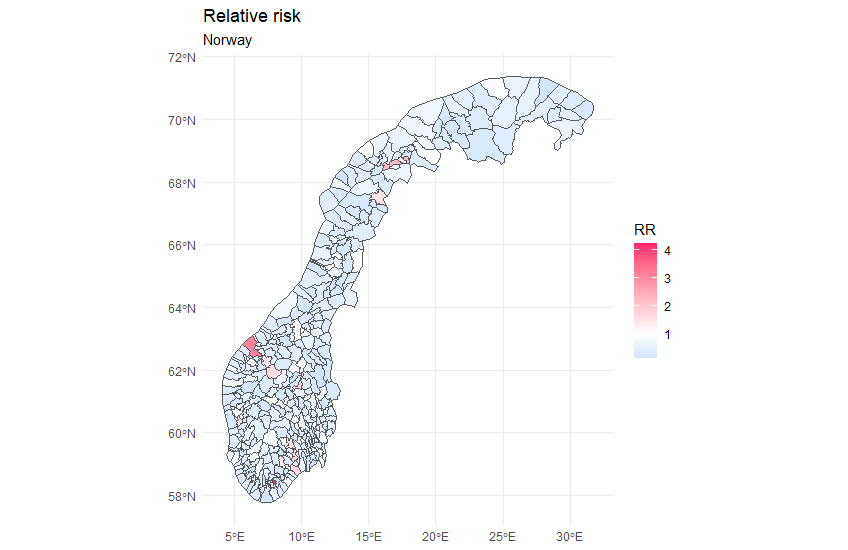
\includegraphics[width = \textwidth]{relative_risk_norway.png}
  \caption{Relative risk of contracting Covid-19 in Norway.}
  \label{rr_norway}
\end{figure}
\begin{figure}[H]
  \centering
  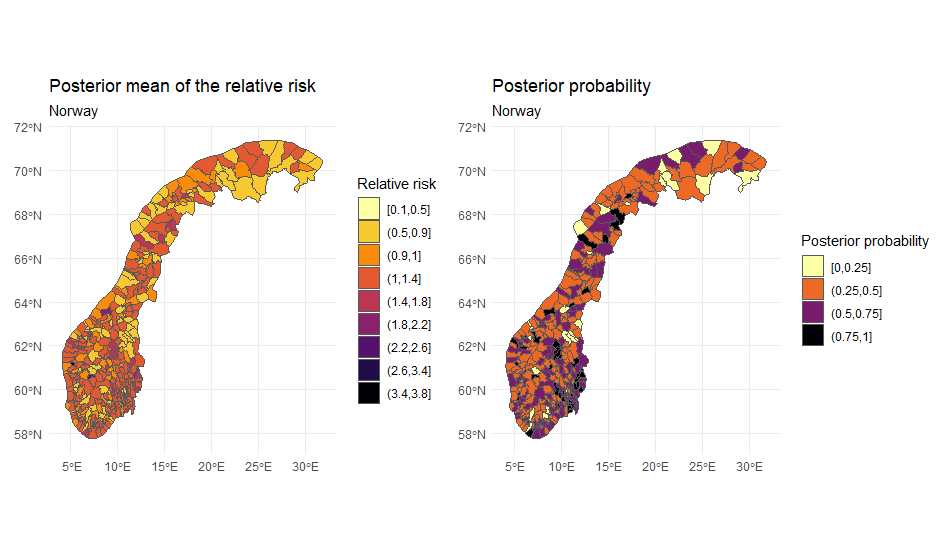
\includegraphics[width = \textwidth]{posterior_norway.png}
  \caption{Posterior mean of the municipality-specific relative risks $\zeta=\exp{\left(\xi\right)}$ compared with the whole of Norway (left) and posterior probability $\mathbb{P}\left(\zeta_i>1|\pmb{y}\right)$}
  \label{posterior_norway}
\end{figure}
\subsection{Discussion of the (Non)-Temporal Models for Germany}
In the non-spatial model for Germany, six coefficients are significant, in addition to the intercept:
\begin{itemize}
    \item The percentage of the vote for the right-wing populist AfD
    \item The population density
    \item The logarithmic trade tax
    \item The percentage of the vote for the SPD
    \item The percentage of the vote for the left-wing party "Die Linke"
    \item The percentage of the vote for the Green party
\end{itemize}
A look at Table~\ref{allGermany} shows that the spatial models outperform the non-spatial model in terms of the DIC and the WAIC, while all models perform about equally well in terms of the CPO. The predictive performance is best for the BYM2 model, just ahead of the proper Besag model, as indicated by the lowest values for the MAE. When adding the spatial term for the BYM2 model, several variables lose their significance, namely the percentage of the vote for the SPD, "Die Linke" and the Greens, while the intercept, the percentage of the vote for the AfD, population density and the logarithmic trade tax remain significant. \\
The exponentiated intercept implies a risk rate of -6.8\% across Germany, which means that the risk of contracting Covid-19 in Germany is 93.2\%.  The greatest influence on the relative risk is determined to be the percentage of the vote for the far-right AfD. An increase in this variable by 1 standard deviation leads to an increase in the relative risk by 25.7\%. The AfD openly criticizes the measures taken by the government in Germany to prevent the spread of Covid-19, which leads to a large proportion of the party's voters not taking the measures seriously and refusing to keep a safe distance or wear a mask in public spaces. Several studies have taken a look at the response of right-wing parties to the pandemic and how people who vote for these types of parties have reacted. Wondreys and Mudde (2020) point out that these parties were quick to warn about the virus, but once cases spiked, they criticized the measures taken to contain the spread of the virus. They noted that right-wing parties often rejected the measures proposed by the leading parties because they themselves are part of the opposition \autocite[][]{wondreys2020victims}, as is the case with the AfD in Germany. Vieten (2020) shows how the far-right mobilizes people for anti-hygiene or anti-lockdown protests and how this is used to normalize the global far-right \autocite[][]{vieten2020new}. Eberl et al. (2020) analysed data from the Austrian Corona Panel Project to test whether populism attitudes and belief in conspiracy theories related to Covid-19 are correlated. Using structural equation modelling, they show that populism indirectly influences Covid-19 conspiracy beliefs through trust in political and scientific institutions. They find that populist attitudes have a negative correlation with trust in the government and the parliament. Furthermore, they find that higher populist attitudes are negatively correlated with trust in science, a factor that reduces belief in Covid-19 conspiracy theories \autocite[][]{eberl2020populism}. Finally, Farias and Pilati (2020) conducted a study in Brazil to predict social distancing violation intention and past non-compliance during the Covid-19 pandemic, controlling for the effects of interolerence of insecurity and socio-demographic variables. Their results included that individuals who support right-wing parties are more likely to violate social distancing measures \autocite[][]{farias2020violating}. \\
An increase in population density by 1 standard deviation leads to a risk increase of 10.9\%. Reasons why a higher population density correlates positively with the number of infections are discussed in Section~\ref{sec:models_norway}. \\
The last significant effect is the logarithmic trade tax with an increase of 1 standard deviation leading to a 6.8\% increase in risk. There are no studies that specifically analyse the relationship between the trade tax and the risk of infection, but some studies have analysed infection rates in different spatial areas while controlling for factors such as income. In general, a negative relationship is found between areas with higher income and infection rates, meaning that areas with higher income had fewer cases of Covid-19. Cordes and Castro (2020) found that postcode areas in New York City with a low proportion of positive tests had higher incomes and tested less compared to lower income areas. They found that people in lower income areas are more likely to be without health insurance \autocite[][]{cordes2020spatial}. Coven and Gupta (2020) found that New York City residents who come from wealthier neighbourhoods are more likely to flee the city, and that people who live in low-income neighbourhoods are more likely to have frontline occupations and visit retail shops more often, increasing their exposure to Covid-19 \autocite[][]{coven2020disparities}. The situation seems to be the same in Europe, as Baena et al. (2020) found that districts in Barcelona with a lower average income had a higher Covid-19 incidence. They found that the incidence in the district with the lowest income is 2.5 times higher than in the district with the highest income \autocite[][]{baena2020impact}. Again, the results of the BYM2 model are not consistent with current research. \\
The relative risk of infection shown in Figure~\ref{rr_germany} is highest in Eastern Germany, more specifically in the federal state of Saxony. Saxony has established itself as the political stronghold of the AfD in recent years, which has even led to the ruling party, the Union, moving further to the right on the political spectrum. In addition to Saxony, the traditionally highly conservative Bavaria and the populous Ruhr region have a relative risk of over 1. Figure~\ref{posterior_germany} shows that for most of these regions the posterior mean of the random effects is over 1, mostly with a posterior probability of at least 0.75.
\begin{figure}[H]
  \centering
  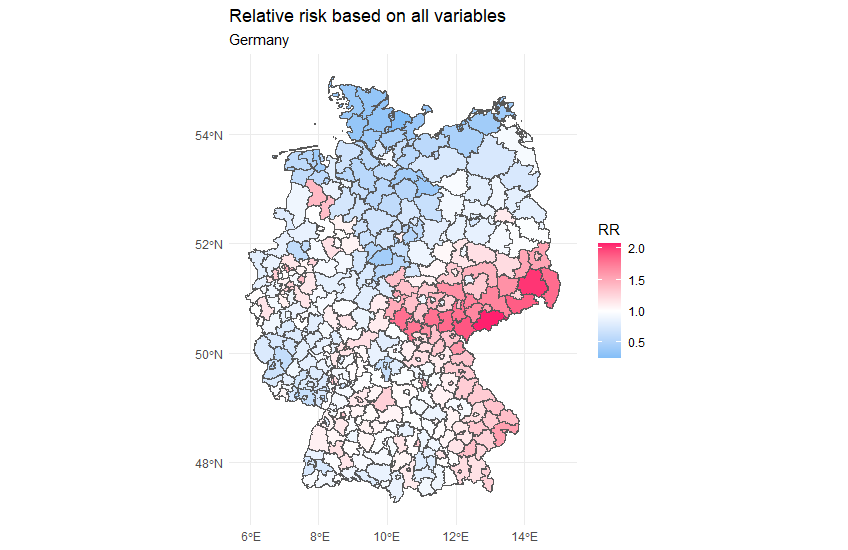
\includegraphics[width = 0.9\textwidth]{relative_risk_germany.png}
  \caption{Relative risk of contracting Covid-19 in Germany.}
  \label{rr_germany}
\end{figure}
\begin{figure}[H]
  \centering
  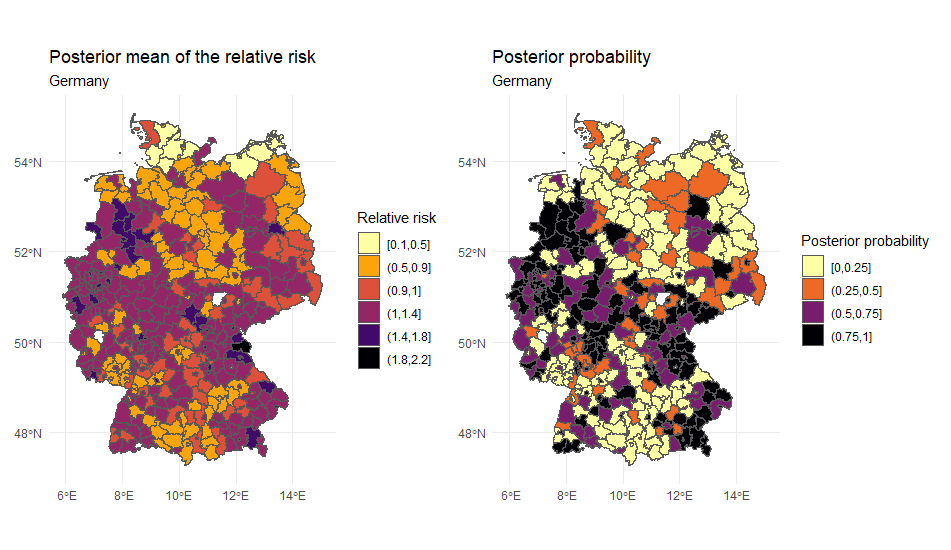
\includegraphics[width = \textwidth]{posterior_germany.png}
  \caption{Posterior mean of the municipality-specific relative risks $\zeta=\exp{\left(\xi\right)}$ compared with the whole of Germany (left) and posterior probability $\mathbb{P}\left(\zeta_i>1|\pmb{y}\right)$}
  \label{posterior_germany}
\end{figure}
\subsection{Comparison Between the Spatial Models and the Predictive Models}
Looking at the predictive models again and comparing them to the spatial models, both Table~\ref{pred_perf} and Table~\ref{pred_perf_norway} show that the predictive models perform significantly worse than the spatial models. For Germany, the test MAE of the random forest is about 80\% higher than that of the BYM2 model, while in Norway it is about 50\% higher. This could indicate that the spatial effect in Norway is not as strong as in Germany, mainly due to the fact that most of the cases in Norway are located in Oslo and the surrounding municipalities. However, the smaller relative difference could be due to the fact that the infection numbers in Norway are significantly lower than in Germany, which naturally leads to a smaller mean absolute error. Nevertheless, the comparison between the two model classes is interesting, as different features turn out to be important for both countries, compared to the BYM2 model for each country. For Germany, it is the number of clinics, the number of public transport platforms and the number of marketplaces, while for Norway it is the number of places of worship, the number of offices, the number of public transport platforms and the number of colleges and universities. For Germany, the logarithmic business tax is the only feature that is important in both models, while for Norway, urban density is the only feature that is important in the BYM2 model and the random forest. \\
Most interesting here, however, is that in both countries the number of public transport platforms is an important factor in explaining infection rates in a municipality. The association between the risk of Covid-19 infection and public transport is well studied. Hu et al. (2021) conducted a study in which they analysed the risk of transmission of the disease on high-speed trains in China. To do this, they used data from around 2300 patients and 72,000 close contacts who had a travel time between 0 and 8 hours from 19 December 2019 to 6 March 2020. They analysed the spatial and temporal distribution of Covid-19 transmission among train passengers to identify associations between infection, spatial distance and travel time. They found a high risk of transmission among train passengers, which showed significant differences depending on travel time and seat position. They suggest reducing the risk of transmission by increasing seat pitch, reducing passenger density and using hygiene equipment \autocite[][]{hu2021risk}. Musselwhite (2020) compares Covid-19 with other infectious diseases that may have similar properties, noting that other types of human coronavirus, e.g. SARS coronavirus or MERS coronavirus, can survive on inanimate surfaces such as metal, glass or plastic for up to nine days and similar surface stability has been observed for SARS-CoV-2. In addition, a link has already been observed between acute respiratory infection (ARI) in winter and the use of buses or trams in the five days before the onset of symptoms. Finally, the greatest risk for infectious diseases on public transport is proximity between people in an enclosed environment. If people do not close their mouths when coughing and sneezing, public transport can become a significant source of microorganisms \autocite[][]{musselwhite2020editorial}.
\clearpage
\section{Discussion of the Temporal Models}
The temporal models for Germany and Norway do not perform as well as hoped. One of the problems for the models is that no distribution is found that fits the data reasonably well. In the end, a negative binomial distribution is used because it seems to fit slightly better than a normal distribution. Especially the QQ-plots in Figure~\ref{fitNegbinomGermany_ts} and Figure~\ref{fitNegbinomNorway_ts} illustrate this problem. The models themselves do not show an unreasonably high value for the MAE of the test data, but this is mainly due to the fact that the test set is kept relatively small with only 20 observations. Table~\ref{germany_temporal_2} shows what happens when the test size for the temporal models for Germany is increased. The MAE in training remains surprisingly low, but the test MAE increases exponentially as the test size increases. 
\begin{table}[H] 
\caption{The performance measures for different types of temporal models for Germany. \label{germany_temporal_2}}
\begin{tabular}{l r r r r r}
\toprule
\textbf{Model}	& Test size & \textbf{$\hbox{MAE}_{\hbox{train}}$} & \textbf{$\hbox{MAE}_{\hbox{test}}$}\ \\
\midrule
Only date as covariate & 20 & 4915 & 27450 \\
Random walk of second order & 20 & 2009 & 6180 \\
AR(1) process & 20 & 18 & 7524 \\
Temporal model &  20 & 1931 & 5821 \\
Only date as covariate & 40 & 4782 & 22559 \\
Random walk of second order & 40 & 1832 & 2090247 \\
AR(1) process & 40 & 7 & 26561 \\
Temporal model &  40 & 1764 & 10457609 \\
Only date as covariate & 60 & 4597 & 22525 \\
Random walk of second order & 60 & 1656 & 5.81e+12 \\
AR(1) process & 60 & 8 & 99471 \\
Temporal model &  60 & 1584 & 5.09e+16 \\
\bottomrule
\end{tabular}
\end{table}
The same effect can be observed for Norway. Even with the small test size, which leads to a low mean absolute error of the test, the quality of the prediction in Germany is not as high, since according to the prognosis the number of infections increases, while in reality the number of infections in Germany decreases. This is illustrated by the comparison between the predicted 7-day incidence and the actual 7-day incidence in Figure~\ref{incidence_germany}, which shows an increase in the predicted 7-day incidence, while in reality the incidence decreases rapidly. For Norway, the comparison between incidences is slightly better, as at least for the last days of the test set, the predicted incidence and the actual incidence both increase as can be seen in Figure~\ref{incidence_norway}. \\
Finally, despite trying a variety of models during this work, hardly any coefficient turned out to be significant and interpretable, as often significant coefficients had values in the tens of thousands. In the models that are ultimately used in this work, the only significant feature besides the intercept turned out to be workplace mobility, with a one standard deviation increase in the mobility leading to a risk increase of 18.6\% in Germany and 20.1\% in Norway. \\
Studies on indoor infection risk are numerous and mostly point to the same thing, namely that aerosols from infected people can effectively transmit the virus indoors. Measures such as wearing face masks and ventilating rooms can reduce the risk of infection, but the most effective measure is still not going to the workplace \autocite[][]{lelieveld2020model, bedford2020covid, hall2020covid}.
% !TEX root = ../my-thesis.tex
%
\chapter{Conclusion}
This research aimed to identify factors that have a significant influence on the spread of Covid-19 in Germany and Norway using Bayesian modelling. Based on the calculated models, it can be concluded that the population density, the percentage of the vote for the right-wing party AfD and the logarithmic trade tax are important factors influencing the spread of the viral disease in Germany. For Norway, it was found that the urban density, the number of unemployed immigrants, the total number of immigrants as well as the number of aerodromes in a municipality and the female to male ratio are important factors. The results indicate that in different countries different factors are influencing infection numbers. It has to be said however, that some of the findings are not in line with current research, specifically the influence of the logarithmic trade tax, the number of aerodromes and the proportion of females. 
blabla why spatio-temporal models were not possible blabla predictive models might make sense for norway bc spatial effect not that strong
% !TEX root = ../my-thesis.tex
%
\chapter{Example Appendix}
\label{sec:appendix}

\Blindtext[1][1]

\section{Appendix Section 1}
\label{sec:appendix:sec1}

\Blindtext[1][1]

\begin{table}[h]
	\begin{tabularx}{\textwidth}{X | X | X}
		%\hline
		Alpha		& Beta			& Gamma			\\ \hline
		0			& 1				& 2				\\ \hline
		3			& 4				& 5				\\ %\hline
	\end{tabularx}
	\label{tab:table1}
	\caption{This is a caption text.}
\end{table}

\section{Appendix Section 2}
\label{sec:appendix:sec2}

\Blindtext[1][1]

\begin{table}[h]
	\begin{tabularx}{\textwidth}{X | X | X}
		%\hline
		Alpha		& Beta			& Gamma			\\ \hline
		0			& 1				& 2				\\ \hline
		3			& 4				& 5				\\ %\hline
	\end{tabularx}
	\label{tab:table2}
	\caption{This is a caption text.}
\end{table}

\Blindtext[1][2]


{%
\setstretch{1.1}
\renewcommand{\bibfont}{\normalfont\small}
\setlength{\biblabelsep}{0pt}
\setlength{\bibitemsep}{0.5\baselineskip plus 0.5\baselineskip}
\printbibliography[nottype=online]
\newrefcontext[labelprefix={@}]
\printbibliography[heading=subbibliography,title={Webpages},type=online]
}
\cleardoublepage

\listoffigures
\cleardoublepage

\listoftables
\cleardoublepage

\lstlistoflistings
\cleardoublepage

\appendix\cleardoublepage
%% !TEX root = ../my-thesis.tex
%
\chapter{Example Appendix}
\label{sec:appendix}

\Blindtext[1][1]

\section{Appendix Section 1}
\label{sec:appendix:sec1}

\Blindtext[1][1]

\begin{table}[h]
	\begin{tabularx}{\textwidth}{X | X | X}
		%\hline
		Alpha		& Beta			& Gamma			\\ \hline
		0			& 1				& 2				\\ \hline
		3			& 4				& 5				\\ %\hline
	\end{tabularx}
	\label{tab:table1}
	\caption{This is a caption text.}
\end{table}

\section{Appendix Section 2}
\label{sec:appendix:sec2}

\Blindtext[1][1]

\begin{table}[h]
	\begin{tabularx}{\textwidth}{X | X | X}
		%\hline
		Alpha		& Beta			& Gamma			\\ \hline
		0			& 1				& 2				\\ \hline
		3			& 4				& 5				\\ %\hline
	\end{tabularx}
	\label{tab:table2}
	\caption{This is a caption text.}
\end{table}

\Blindtext[1][2]
       % INCLUDE: appendix
\cleardoublepage
%% !TEX root = ../my-thesis.tex
%
%************************************************
% Declaration
%************************************************
\pdfbookmark[0]{Declaration}{Declaration}
\addchap{Declaration}
\label{sec:declaration}
\thispagestyle{empty}

You can put your declaration here, to declare that you have completed your work solely and only with the help of the references you mentioned.

\bigskip

\noindent\textit{\thesisUniversityCity, \thesisDate}

\smallskip

\begin{flushright}
	\begin{minipage}{5cm}
		\rule{\textwidth}{1pt}
		\centering\thesisName
	\end{minipage}
\end{flushright}

%*****************************************
%*****************************************

\clearpage

\newpage
\mbox{}

% **************************************************
% End of Document CONTENT
% **************************************************
\end{document}
